% This template is created by SV Bùi Vân Anh, và Thầy Nguyễn Tiến Hòa từ phòng Lab xử lý tín hiệu băng gốc hệ thống 5G. Chúng tôi rất vui nếu được nhắc đến trong lời cảm ơn.
%%%%%%%%%%%%%%%%%%%%%%%%%%%%%%%%%%%%%%%%%%%%%%%%%%%%%%%
\documentclass{article} % Tạo một bản báo cáo
\usepackage[utf8]{inputenc}
\usepackage[T5]{fontenc} % Để sử dụng Tiếng Việt
\usepackage[fontsize=13pt]{scrextend} % Set fontsize=13pt
%\usepackage[paperheight=29.7cm,paperwidth=21cm,right=2cm,left=3cm,top=2cm,bottom=2.5cm]{geometry}% Chuẩn A4, căn lề phải, trái, trên, dưới.
\usepackage[paperheight=29.7cm,paperwidth=21cm,right=2cm,left=3cm,top=2cm,bottom=2.5cm,twoside]{geometry}% Chuẩn A4, căn lề phải, trái, trên, dưới.
\usepackage{svg}
\usepackage{amsmath}
\usepackage{mathptmx} % Time New Roman
\usepackage{graphicx} % Thư viện chèn ảnh
\usepackage{float} % Set vị trí chèn ảnh
\usepackage{tikz} % Thư viện tạo khung bìa
\usepackage{parskip}
\usepackage{slashbox}
\usepackage{multirow}

\usetikzlibrary{calc} % Thư viện tikz
\usepackage{indentfirst} % Thư viện thụt đầu dòng
\renewcommand{\baselinestretch}{1.2} % Giãn dòng 1.2
\setlength{\parskip}{6pt} % Spacing after
\setlength{\parindent}{15pt} % Set khoảng cách thụt đầu dòng mỗi đoạn
\usepackage{titlesec} % Thư viện để set up các kiểu chữ
\setcounter{secnumdepth}{4} % 4 Heading
\titlespacing{\section}{0pt}{0pt}{30pt} % Heading 1
\titleformat*{\section}{\fontsize{16pt}{0pt}\selectfont \bfseries \centering}

\titlespacing{\subsection}{0pt}{\parskip}{0.6\parskip} % Heading 2
\titleformat*{\subsection}{\fontsize{14pt}{0pt}\selectfont \bfseries}

\titlespacing{\subsubsection}{0pt}{\parskip}{0.6\parskip} % Heading 3
\titleformat*{\subsubsection}{\fontsize{13pt}{0pt}\selectfont \bfseries \itshape}

\titlespacing{\paragraph}{0pt}{\parskip}{0.6\parskip}  % Heading 4
\titleformat{\paragraph}{\fontsize{13pt}{0pt}\selectfont \itshape}{\theparagraph}{1em}{}

\renewcommand{\figurename}{\fontsize{12pt}{0pt}\selectfont \bfseries Hình}
\renewcommand{\thefigure}{\thesection.\arabic{figure}}
\usepackage[font=bf]{caption}
\captionsetup[figure]{labelsep=space}

\renewcommand{\tablename}{\fontsize{12pt}{0pt}\selectfont \bfseries Bảng}
\renewcommand{\thetable}{\thesection.\arabic{table}}
\captionsetup[table]{labelsep=space}

\usepackage{makecell}
\usepackage{array}
\newcolumntype{P}[1]{>{\centering \arraybackslash \fontsize{12pt}{0pt}\selectfont }m{#1}}
\newcolumntype{M}[1]{>{\centering\arraybackslash}m{#1}} % thêm ...

\newcommand{\mkc}[1]{\textbf{\makecell{#1}}}

\usepackage{tabularx, booktabs}
\newcolumntype{s}{>{\hsize=.3\hsize}X}
\newcolumntype{y}{>{\hsize=.4\hsize}X}
\newcolumntype{d}{>{\hsize=.1\hsize}X}
\newcolumntype{a}{>{\hsize=1.1\hsize}X}
\newcolumntype{g}{>{\hsize=5\hsize}X}
\renewcommand{\tabularxcolumn}[1]{>{\small}m{#1}}

\renewcommand{\theequation}{\thesection.\arabic{equation}} % Thay đổi đánh số phương trình mặc định
\newtheorem{theorem}{Định lý}[section]
\newtheorem{defn}[theorem]{Định nghĩa}
\newtheorem{corollary}[theorem]{Hệ quả}
\newtheorem{lemma}[theorem]{Bổ đề}

\usepackage{lipsum} % Thư viện tạo chữ linh tinh.
\renewcommand{\contentsname}{MỤC LỤC}
\renewcommand{\listfigurename}{DANH MỤC HÌNH VẼ}
\renewcommand{\listtablename}{DANH MỤC BẢNG BIỂU}
\renewcommand{\refname}{TÀI LIỆU THAM KHẢO}

\usepackage[unicode]{hyperref}
\usepackage{bookmark}
\usepackage{colortbl}
\definecolor{LightCyan}{rgb}{0.88,1,1}
\usepackage{forloop}
\newcounter{loopcntr}
\newcommand{\rpt}[2][1]{\forloop{loopcntr}{0}{\value{loopcntr}<#1}{#2}}

\begin{document}

\begin{titlepage}
\begin{tikzpicture}[overlay,remember picture]
\draw [line width=3pt]
    ($ (current page.north west) + (3.0cm,-2.0cm) $)
    rectangle
    ($ (current page.south east) + (-2.0cm,2.5cm) $);
\draw [line width=0.5pt]
    ($ (current page.north west) + (3.1cm,-2.1cm) $)
    rectangle
    ($ (current page.south east) + (-2.1cm,2.6cm) $); 
\end{tikzpicture}
\begin{center}
\vspace{-12pt}  TRƯỜNG ĐẠI HỌC BÁCH KHOA HÀ NỘI \\
\textbf{\fontsize{16pt}{0pt}\selectfont VIỆN ĐIỆN TỬ - VIỄN THÔNG}
\vspace{0.5cm}
 \begin{figure}[H]
     \centering
     \includegraphics[width=1.53cm,height=2.26cm]{Images/logodhbk.png}
 \end{figure}
\vspace{1.5cm}
\fontsize{24pt}{0pt}\selectfont ĐỒ ÁN\\
\vspace{12pt}
\textbf{\fontsize{32pt}{0pt}\selectfont TỐT NGHIỆP ĐẠI HỌC}
\vspace{1.5cm}
\end{center}
\hspace{6pt}\textbf{\fontsize{14pt}{0pt}\selectfont Đề tài:}
\begin{center}
    \textbf{\fontsize{20pt}{0pt}\selectfont THIẾT KẾ BỘ CHUYỂN ĐỔI}\\
    \vspace{0.3cm}
    \textbf{\fontsize{20pt}{0pt}\selectfont PDM SANG PCM}

\vspace{1.5cm}
\begin{table}[H]
    \centering
    \begin{tabular}{l l}
 \fontsize{14pt}{0pt}\selectfont Sinh viên thực hiện:    & \fontsize{14pt}{0pt}\selectfont NGUYỄN VIỆT THI \vspace{6pt} \\ 
     &\fontsize{14pt}{0pt}\selectfont Lớp Điện tử 10 - K63 \vspace{6pt}\\
\fontsize{14pt}{0pt}\selectfont Giảng viên hướng dẫn: & \fontsize{14pt}{0pt}\selectfont PGS. TS. Nguyễn Đức Minh
\end{tabular}
\end{table}
\vspace{3.5cm}
 \fontsize{14pt}{0pt}\selectfont Hà Nội, 02/2023
\end{center}
\end{titlepage}
\cleardoublepage
 % Bìa đồ án.
\begin{titlepage}
% Tạo khung trang bìa đầu tiên 
\begin{tikzpicture}[overlay,remember picture]
\draw [line width=3pt]
    ($ (current page.north west) + (3.0cm,-2.0cm) $)
    rectangle
    ($ (current page.south east) + (-2.0cm,2.5cm) $);
\draw [line width=0.5pt]
    ($ (current page.north west) + (3.1cm,-2.1cm) $)
    rectangle
    ($ (current page.south east) + (-2.1cm,2.6cm) $); 
\end{tikzpicture}

% Tạo chữ cho khung bìa 
\begin{center}\vspace{-15pt}
TRƯỜNG ĐẠI HỌC BÁCH KHOA HÀ NỘI \\
\textbf{\underline{\fontsize{16pt}{0pt}\selectfont TRƯỜNG ĐIỆN - ĐIỆN TỬ}}

\vspace{0.5cm}
\begin{figure}[H]
    \centering
    \includegraphics[width=1.53cm, height=2.26cm]{Images/logodhbk.png}
\end{figure}
\vspace{1.2cm}

\fontsize{24pt}{0pt}\selectfont ĐỒ ÁN \\[12pt] 
\textbf{\fontsize{32pt}{0pt}\selectfont TỐT NGHIỆP ĐẠI HỌC} 
\vspace{1.2cm}

\end{center}
\hspace{12pt}\textbf{\fontsize{14pt}{0pt}\selectfont Đề tài:}
\begin{center}
    \textbf{\fontsize{20pt}{0pt}\selectfont THIẾT KẾ, TỔNG HỢP VÀ TRIỂN KHAI \\}
   \textbf{\fontsize{20pt}{0pt}\selectfont BỘ CHUYỂN ĐỔI PDM SANG PCM\\}
    % \textbf{\fontsize{20pt}{0pt}\selectfont ỨNG DỤNG TRONG XỬ LÝ ÂM THANH \\}

    
\vspace{2cm}    

    \begin{tabular}{ l l }
        \fontsize{14pt}{0pt}\selectfont Sinh viên thực hiện: & \fontsize{14pt}{0pt}\selectfont NGUYỄN VIỆT THI  \vspace{0.2cm} \\ 
        & \fontsize{14pt}{0pt}\selectfont MSSV: 20182798 \vspace{0.2cm}\\
        & \fontsize{14pt}{0pt}\selectfont Lớp: Điện tử 10 - K63 \vspace{0.2cm}\\
        \fontsize{14pt}{0pt}\selectfont Giảng viên hướng dẫn: &  \fontsize{14pt}{0pt}\selectfont  PGS. TS. NGUYỄN ĐỨC MINH\vspace{0.2cm}\\
                \fontsize{14pt}{0pt}\selectfont Cán bộ phản biện: &  \fontsize{14pt}{0pt}\selectfont  
    \end{tabular} \\[3cm]
    \fontsize{14pt}{0pt}\selectfont Hà Nội, 03-2023
\end{center}
\end{titlepage} \cleardoublepage % Bìa đồ án.

% ĐÁNH GIÁ CỦA CÁN BỘ HƯỚNG DẪN
{
\begin{center}\vspace{-15pt}
\fontsize{12pt}{0pt}\selectfont TRƯỜNG ĐẠI HỌC BÁCH KHOA HÀ NỘI \\
\vspace{0.2cm}
\textbf{\underline{\fontsize{12pt}{0pt}\selectfont TRƯỜNG ĐIỆN - ĐIỆN TỬ}}
\vspace{1.0cm}
\end{center}

\section*{\fontsize{14pt}{0pt}\selectfontĐÁNH GIÁ QUYỂN ĐỒ ÁN TỐT NGHIỆP\\\fontsize{12pt}{0pt}\selectfont \vspace{4pt}\textbf{(DÀNH CHO CÁN BỘ HƯỚNG DẪN)}}
\thispagestyle{empty}
% \vspace{-10pt}

\noindent Tên đề tài: THIẾT KẾ, TỔNG HỢP VÀ TRIỂN KHAI BỘ CHUYỂN ĐỔI PDM SANG PCM \\
\vspace{0.2cm}
% \noindent\vbox spread 6pt {}\null\xleaders \hbox to 2mm {\hss . \hss}\hfill \null \\
\vspace{0.2cm}
\noindent Họ và tên SV: NGUYỄN VIỆT THI \hspace{3cm} MSSV: 20182798 \\
\noindent Cán bộ hướng dẫn: PGS. TS. NGUYỄN ĐỨC MINH \\

\begin{table}[H]
    \centering
    \begin{tabular}{
    | P{0.05\linewidth} 
    | P{0.13\linewidth} 
    | P{0.63\linewidth} 
    | P{0.08\linewidth} |
    }
    \hline
        \textbf{STT}& \textbf{Tiêu chí \qquad \qquad \textnormal{(Điểm tối đa)}} & \textbf{Hướng dẫn đánh giá tiêu chí} & \textbf{Điểm tiêu chí} \\\hline

        \multirow{2}{*}{1} & \multirow{2}{*}{\parbox{2.15cm}{\vspace{0.2cm}\centering \textbf{Thái độ làm việc \qquad \quad (2.5 điểm)}}} & \raggedright Nghiêm túc, tích cực và chủ động trong quá trình làm ĐATN & \multirow{2}{*}{} \\ \cline{3-3}
         & & \raggedright Hoàn thành đầy đủ và đúng tiến độ các nội dung được GVHD giao & \\\hline 

         \multirow{2}{*}{2} & \multirow{2}{*}{\parbox{2.15cm}{\vspace{0.1cm}\centering \textbf{Kỹ năng viết quyển ĐATN \\ (2 điểm)}}} & \raggedright Trình bày đúng mẫu quy định, bố cục các chương logic và hợp lý: Bảng biểu, hình ảnh rõ ràng, có tiêu đề, được đánh số thứ tự và được giải thích hay đề cập đến trong đồ án, có căn lề, dấu cách sau dấu chấm, dấu phẩy, có mở đầu chương và kết luận chương, có liệt kê tài liệu tham khảo và có trích dẫn, v.v. & \multirow{2}{*}{} \\ \cline{3-3}
         & & \raggedright Kỹ năng diễn đạt, phân tích, giải thích, lập luận: Cấu trúc câu rõ ràng, văn phong khoa học, lập luận logic và có cơ sở, thuật ngữ chuyên ngành phù hợp, v.v. & \\\hline 

         \multirow{3}{*}{3} & \multirow{3}{*}{\parbox{2.15cm}{\vspace{0.1cm}\centering \textbf{Nội dung và kết quả đạt được \qquad \quad (5 điểm)}}} & \raggedright Nêu rõ tính cấp thiết, ý nghĩa khoa học và thực tiễn của đề tài, các vấn đề và các giả thuyết, phạm vi ứng dụng của đề tài. Thực hiện đầy đủ quy trình nghiên cứu: Đặt vấn đề, mục tiêu đề ra, phương pháp nghiên cứu/ giải quyết vấn đề, kết quả đạt được, đánh giá và kết luận. & \multirow{3}{*}{} \\ \cline{3-3}
         & & \raggedright Nội dung và kết quả được trình bày một cách logic và hợp lý, được phân tích và đánh giá thỏa đáng. Biện luận phân tích kết quả mô phỏng/ phần mềm/ thực nghiệm, so sánh kết quả đạt được với kết quả trước đó có liên quan. & \\ \cline{3-3}
         & & \raggedright Chỉ rõ phù hợp giữa kết quả đạt được và mục tiêu ban đầu đề ra đồng thời cung cấp lập luận để đề xuất hướng giải quyết có thể thực hiện trong tương lai. Hàm lượng khoa học/ độ phức tạp cao, có tính mới/tính sáng tạo trong nội dung và kết quả đồ án. & \\\hline  
         
    \end{tabular}
\end{table}

\begin{table}[H]
    \centering
    \begin{tabular}{
    | P{0.05\linewidth} 
    | P{0.13\linewidth} 
    | P{0.63\linewidth} 
    | P{0.08\linewidth} |
    }
    \hline
         \multirow{2}{*}{4} & \multirow{2}{*}{\parbox{2.15cm}{\vspace{0.1cm}\centering \textbf{Điểm thành tích \qquad \qquad(1 điểm)}}} & \raggedright Có bài báo KH được đăng hoặc chấp nhận đăng/ đạt giải SV NCKH giải 3 cấp Trường trở lên/ Các giải thưởng khoa học trong nước, quốc tế từ giải 3 trở lên/ Có đăng ký bằng phát minh sáng chế. \textbf{(1 điểm)} & \multirow{2}{*}{} \\ \cline{3-3}
         & & \raggedright Được báo cáo tại hội đồng cấp Trường trong hội nghị SV NCKH nhưng không đạt giải từ giải 3 trở lên/ Đạt giải khuyến khích trong cuộc thi khoa học trong nước, quốc tế/ Kết quả đồ án là sản phẩm ứng dụng có tính hoàn thiện cao, yêu cầu khối lượng thực hiện lớn. \textbf{(0,5 điểm)} & \\\hline 
         & & \raggedleft \textbf{Điểm tổng các tiêu chí:} & \\\hline
         & & \raggedleft \textbf{Điểm hướng dẫn:} & \\\hline
    \end{tabular}
\end{table}

% \hspace{9cm} Ngày: ... / ... / 20...

\vspace{0.3cm}

\hspace{9.0cm}\textbf{Cán bộ hướng dẫn}

\hspace{9cm}(Ký và ghi rõ họ tên)
\cleardoublepage
} % Đánh giá quyển đồ án tốt nghiệp cho giảng viên hướng dẫn và cán bộ phản biện.
\input{PhanDau/DanhGiaHoiDong}
\section*{LỜI NÓI ĐẦU}
\thispagestyle{empty}
MEMS (Microelectromechanical Systems) microphone là một loại microphone được sử dụng phổ biến trong các ứng dụng di động, thiết bị IoT (Internet of Things) và các hệ thống điều khiển giọng nói. Với kích thước nhỏ gọn và tiêu thụ điện năng thấp, MEMS microphone đã thay thế các loại microphone truyền thống và trở thành một công nghệ quan trọng trong ngành công nghiệp âm thanh.

MEMS microphone hoạt động bằng cách chuyển đổi sóng âm thành tín hiệu điện thông qua các cảm biến nhỏ được tích hợp trên một vi mạch nhỏ. Sự khác biệt của nó so với các loại microphone khác là chúng sử dụng kỹ thuật Pulse Density Modulation (PDM) để chuyển đổi tín hiệu tương tự sang số. PDM cho phép các tín hiệu âm thanh được biểu diễn bằng mật độ xung, giúp giảm thiểu tối đa nhiễu và giảm độ trễ trong việc xử lý tín hiệu.

Ngoài ra, MEMS microphone còn có nhiều ưu điểm khác như độ nhạy cao, khả năng tái tạo âm thanh chính xác và khả năng giảm tiếng ồn tốt. Với những ưu điểm này, MEMS microphone trở thành một công nghệ quan trọng trong việc cải thiện chất lượng âm thanh trong các sản phẩm điện tử tiêu dùng, từ điện thoại thông minh, máy tính bảng, đồng hồ thông minh cho đến loa thông minh và các thiết bị đo lường.

Với sự phát triển của công nghệ, MEMS microphone dự kiến sẽ tiếp tục cải tiến và phát triển để đáp ứng nhu cầu ngày càng cao về chất lượng âm thanh và tiêu thụ năng lượng thấp trong các ứng dụng di động và IoT (Internet of Things).

Nhận thấy được tiềm năng to lớn đó, cũng như qua những trải nghiệm thực tế và kiến thức được tiếp thu trong suốt quá trình học tập tại Đại Học Bách Khoa Hà Nội, em đã lựa chọn, tìm hiểu, nghiên cứu về bộ chuyển đổi PDM (Pulse density modulation) sang PCM (Pulse-code modulation) bằng thiết kế số và đưa vào đồ án tốt nghiệp.

Em xin chân thành cảm ơn  \textbf{PGS. TS. NGUYỄN ĐỨC MINH} - giảng viên Trường Điện –
Điện tử, Đại học Bách Khoa Hà Nội đã tận tình dẫn dắt, đưa ra 
các nhận xét trong quá trình thực thi đồ án. Đồng thời, em cũng cảm ơn anh \textbf{Nguyễn Hải Anh}, anh \textbf{Tạ Xuân Tùng} và công ty \textbf{Dolphin Technology Viet Nam Center} đã nhiệt tình hướng dẫn, tạo điều kiện và hỗ trợ các công cụ, thiết bị thiết kế để em có thể hoàn thiện dự án này. Do kiến thức còn hạn chế nên đề tài không tránh khỏi thiếu sót và sơ suất. Em rất mong nhận được các ý kiến đóng góp, nhận xét của các thầy cô để đề tài được hoàn thiện và chỉn chu hơn.

Em xin chân thành cảm ơn !

\hspace{7cm}Hà Nội, ngày 03 tháng 03 năm 2023

\newpage % Lời nói đầu.

\section*{LỜI CAM ĐOAN}
\thispagestyle{empty}
Tôi là NGUYỄN VIỆT THI, mã số sinh viên 20182798, sinh viên lớp Điện tử 10, khóa 63. Giảng viên hướng dẫn là PGS.TS. NGUYỄN ĐỨC MINH. Tôi xin cam đoan toàn bộ nội dung được trình bày trong đồ án “THIẾT KẾ, TỔNG HỢP VÀ TRIỂN KHAI BỘ CHUYỂN ĐỔI PDM SANG PCM” là kết quả quá trình tìm hiểu và nghiên cứu của tôi. Các dữ liệu được nêu trong đồ án là hoàn toàn trung thực, phản ánh đúng kết quả đo đạc thực tế. Mọi thông tin trích dẫn đều tuân thủ các quy định về sở hữu trí tuệ; các tài liệu tham khảo được liệt kê rõ ràng. Tôi xin chịu hoàn toàn trách nhiệm với những nội dung được viết trong đồ án này.

\vspace{6pt}
\hspace{8.3cm}Hà Nội, ngày 03 tháng 03 năm 2023

\hspace{9.5cm}\textbf{Người cam đoan}

\vspace{2cm}
\hspace{9.15cm}\textbf{NGUYỄN VIỆT THI}
% \cleardoublepage
\newpage % Lời cam đoan.

 % Tạo mục lục tự động
\addtocontents{toc}{\protect\thispagestyle{empty}}
\tableofcontents 
\thispagestyle{empty}
\cleardoublepage

\pagenumbering{roman} % Đánh số thứ tự la mã
\section*{DANH MỤC KÝ HIỆU VÀ CHỮ VIẾT TẮT}
\phantomsection \addcontentsline{toc}{section}{\numberline {} DANH MỤC KÝ HIỆU VÀ CHỮ VIẾT TẮT}

\begin{tabular}{ l l }
\hspace{1cm} DAC & \hspace{4cm} Digital analog converter \\  
\hspace{1cm} DAC& \hspace{4cm} Analog digital converter    \\
\hspace{1cm} DS  & \hspace{4cm} Delta-Sigma\\
\hspace{1cm} FIR & \hspace{4cm} Finite Impulse Response \\  
\hspace{1cm} CIC & \hspace{4cm} Cascaded Integrator Comb \\  

\end{tabular}  

\newpage % Danh mục ký hiệu và chữ viết tắt

%Tạo danh mục hình vẽ.
{\let\oldnumberline\numberline
\renewcommand{\numberline}{Hình~\oldnumberline}
\listoffigures} 
\phantomsection\addcontentsline{toc}{section}{\numberline {} DANH MỤC HÌNH VẼ}
\newpage

 %Tạo danh mục bảng biểu.
{\let\oldnumberline\numberline
\renewcommand{\numberline}{Bảng~\oldnumberline}
\listoftables}
\phantomsection\addcontentsline{toc}{section}{\numberline {} DANH MỤC BẢNG BIỂU}
\newpage

\phantomsection\addcontentsline{toc}{section}{\numberline {}TÓM TẮT ĐỒ ÁN}
\section*{TÓM TẮT ĐỒ ÁN}
Các micro kỹ thuật số là một trong những cảm biến phổ biến nhất được sử dụng trong đời sống hàng ngày của con người. Micro kỹ thuật số MEMS thường có đầu ra theo mã hoá mật độ xung (PDM) và đầu ra cần được biến thành mã hoá mã xung (PCM) để phân tích tiếp. Đồ án này trình bày một hệ thống chuyển đổi tín hiệu PDM sang PCM được thực hiện trên phần cứng. Quá trình chuyển đổi được thực hiện bằng các bộ lọc CIC (Cascaded Integrator Comb), Half-Band và FIR (Finite Impulse Response).
% \cleardoublepage
\newpage

\phantomsection\addcontentsline{toc}{section}{\numberline {}ABSTRACT}
\section*{ABSTRACT}
The digital microphone are one of the most common sensors used in people's daily life. MEMS digital microphones often produce pulse density coded (PDM) output, which must be transformed to pulse coding (PCM) for further research. This project demonstrates a hardware-based PDM to PCM signal conversion technology. Using CIC (Cascaded Integrator Comb), Half-Band, and FIR (Finite Impulse Response) filters, the conversion is carried out.
% \cleardoublepage
\newpage % Tóm tắt đồ án 

\pagenumbering{arabic} % Đánh số thứ tự 1,2,3...
% \phantomsection\addcontentsline{toc}{section}{\numberline {}CHƯƠNG 1.  CHƯƠNG MỞ ĐẦU}
\section*{CHƯƠNG 1.  CHƯƠNG MỞ ĐẦU}
Phần mở đầu giới thiệu vấn đề mà đồ án cần giải quyết, mô tả được các phương pháp hiện có để giải quyết vấn đề, trình bày mục đích của đồ án song song với việc giới hạn phạm vi của vấn đề mà đồ án sẽ tập trung giải quyết. Phần này cũng sẽ giới thiệu tóm tắt cấu trúc đồ án và nội dung tương ứng của các phần sẽ lần lượt được trình bày ở các chương tiếp theo.

Nội dung chính của một đồ án tốt nghiệp thường bao gồm:
\begin{itemize}
    \item Phần mở đầu giới thiệu đề tài.
    \item Một chương giới thiệu cơ sở lý thuyết.
    \item Một hoặc nhiều chương trình bày các vấn đề về tính toán và thiết kế.
    \item Một chương mô tả các thí nghiệm và kết quả thu được.
\end{itemize}
\newpage
% \phantomsection\addcontentsline{toc}{section}{\numberline {}CHƯƠNG 2.  CƠ SỞ LÝ THUYẾT}
\section*{CHƯƠNG 2. CƠ SỞ LÝ THUYẾT} \label{chuong2}
\setcounter{section}{2}
\setcounter{figure}{0}
\setcounter{table}{0}
Chương này sẽ trình bày tổng quan về hệ thống xử lý âm thanh số. Các khái niệm, cơ sở lý thuyết về bộ chuyển đổi tương tự số (Sigma-Delta), các kỹ thuật xử lý tín hiệu trên nhiều miền tần số, các bộ lọc tiết kiệm tài nguyên có thể ứng dụng và triển khai trên phần cứng, \ldots sẽ lần lượt được làm rõ trong chương này. Các kiến thức nền tảng được trình bày dựa trên quá trình tìm hiểu tổng hợp các nguồn tài liệu có tính xác minh cao được liệt kê dưới phần tài liệu tham khảo.

\subsection{ Lý thuyết điều chế Sigma Delta và Pulse Density Modulation}
Tín hiệu âm thanh là một dạng tín hiệu điện tử được tạo ra bởi dao động cơ học của màng nhạy cảm âm thanh ví dụ như loa hay micro. Khi âm thanh được tạo ra, nó là các dao động cơ học của các đối tượng trong không gian xung quanh, chẳng hạn như giọng nói, nhạc cụ, tiếng động, và âm thanh môi trường tự nhiên. Các dao động này được chuyển đổi thành tín hiệu điện tử bằng các thiết bị thu âm, điển hình là micro hoặc đầu đọc đĩa, sau đó được xử lý để tạo ra một tín hiệu âm thanh tương ứng.

Trong một hệ thống xử lí tín hiệu âm thanh số (hình \ref{hinh21}), âm thanh ban đầu là dạng tín hiệu tương tự  được đưa qua bộ chuyển đổi tương tự số (ADC) để số hóa dưới dạng tín hiệu số. Tín hiệu đó tiếp tục được xử lý qua bộ xử lý tín hiệu số để đáp ứng được các yêu cầu cần thiết, sau đó đưa về tín hiệu tương tự để phát thông qua bộ biến đổi số tương tự (DAC). 

\begin{figure}[!ht]
    \centering
    
    \includegraphics[width=15cm]{Images/top.png}
    \caption[Sơ đồ khối của hệ thống]{\bfseries \fontsize{12pt}{0pt}\selectfont Sơ đồ tổng quan hệ thống xử lí âm thanh số}
    \label{hinh21}
\end{figure}

Quá trình số hóa gồm 3 bước theo thứ tự sau: lấy mẫu, lượng tử và mã hóa. Trong đó, lấy mẫu là lấy các giá trị của tín hiệu tại các thời điểm rời rạc. Do đó, lấy mẫu còn gọi là rời rạc hóa. Tiếp theo, lượng tử hóa là làm gần đúng giá trị của tín hiệu tại thời điểm lấy mẫu với các mức lượng tử (giá trị rời rạc). Lượng tử hóa được xác định bởi độ chính xác của máy tính. Cuối cùng, mã hóa là biểu diễn một số theo hệ thống nhị phân mà máy tính có thể đọc được \cite{xulytinhieusobook}. Ba quá trình trên sẽ được tích hợp và thực hiện trên bộ ADC.

Bộ chuyển đổi tương tự số có 3 kiến trúc phổ biến hiện tại đang được sử dụng là 
Sigma Delta ADC, Successive Approximation ADC (SAR ADC) và Pipelined ADC.
Mỗi kiến trúc có các đặc điểm khác nhau – một số tốt hơn trong việc hỗ trợ độ chính xác của độ phân giải cao, trong khi những kiến trúc khác hỗ trợ tốt hơn cho tốc độ lấy mẫu cao (bảng \ref{bang21}). Cho nên mỗi kiến trúc sẽ được sử dụng trong các ứng dụng khác nhau.
\begin{table}[h!]
\centering
\caption[So sánh giữa các kiến trúc ADC]{\bfseries\fontsize{12pt}{0pt}\selectfont So sánh giữa các kiến trúc ADC}
\begin{tabular}{|c|c|c|c|}
\hline 
\bfseries  Kiến trúc   &\bfseries Tốc độ lấy mẫu   &\bfseries Độ phân giải \hspace{0pt}   & \bfseries Khác\hspace{0pt}\\
\hline 
\multicolumn{1}{|l|}{\begin{tabular}[c]{@{}l@{}}\textbf{SAR}\\ ADS7xxx\\ ADS8xxx\end{tabular}} & \multicolumn{1}{l|}{\begin{tabular}[c]{@{}l@{}}$\leq 4 Msps$\\ $\leq 1.25 Msps$\end{tabular}} & \multicolumn{1}{l|}{\begin{tabular}[c]{@{}l@{}}$\leq 16 bit$\\ $\leq 18 bit$\end{tabular}} & \multicolumn{1}{l|}{\begin{tabular}[c]{@{}l@{}}Dễ dàng sử dụng\\ Độ trễ bằng 0\\ Công suất thấp\end{tabular}} \\ \hline
\multicolumn{1}{|l|}{\begin{tabular}[c]{@{}l@{}}\textbf{Delta-Sigma}\\ ADS10xx/11xx\\ ADS12xx\\ ADS13xx\\ ADS16xx\end{tabular}} & \multicolumn{1}{l|}{\begin{tabular}[c]{@{}l@{}}$\leq 4 Ksps$\\ $\leq 4 Msps$\\ $\leq 10 Msps$\end{tabular}} & \multicolumn{1}{l|}{\begin{tabular}[c]{@{}l@{}}$> 24 bit$\\ $\leq 24 bit$\\ $\leq 16 bit$\end{tabular}} & \multicolumn{1}{l|}{\begin{tabular}[c]{@{}l@{}}Độ phân giải cao\\ Tính tích hợp cao\end{tabular}} \\ \hline
\multicolumn{1}{|l|}{\textbf{Pipeline}} & \multicolumn{1}{l|}{\begin{tabular}[c]{@{}l@{}}$\leq 200 Msps$\\ $\leq 250 Msps$\\ $\leq 1000 Msps$\end{tabular}} & \multicolumn{1}{l|}{\begin{tabular}[c]{@{}l@{}}$\leq 16 bit$\\ $\leq 14 bit$\\ $\leq 12 bit$\end{tabular}} & \multicolumn{1}{l|}{\begin{tabular}[c]{@{}l@{}}Tốc độ cao\\ Công suất cao\end{tabular}} \\ \hline
\end{tabular} 
\label{bang21}
\end{table}

Vì dải âm thanh nghe trong ngưỡng nghe có tần số không cao (20 – 20000 Hz) nằm trong khả năng lấy mẫu của bộ điều chế Delta Sigma và trong các ứng dụng âm thanh được mã hóa trong khoảng từ 16 – 24 bit. Do đó, kiến trúc Delta Sigma sẽ phù hợp cho việc số hóa âm thanh hơn các kiến trúc còn lại.

Một thiết bị điển hình sử dụng kiến trúc Sigma Delta (SD) là MEMS Microphone, 
(MicroelectromechanicalSystem Microphone) thiết bị này có thể được tìm thấy phổ biến trên các điện thoại di động, các máy ghi âm hoặc các thiết bị thu thanh không sử yêu cầu về chất lượng âm thanh quá cao nhưng giá thành rẻ và phù hợp với yêu cầu sử dụng. Tín hiệu thu được trên MEMS Microphone có dạng tín hiệu Pulse Density Modulation (PDM), là dạng 1 bit và truyền với tần số cao, giao thức truyền tương ứng có tên là PDM Interface. Một số MEMS Microphone sử dụng giao thức truyền âm thanh là I2S nhưng chỉ là số ít, phần lớn sử dụng PDM.
\begin{figure}[!ht]
    \centering
    \includesvg[width=13cm]{Images/Chuong2/sinewave_to_pdm.svg}
    \caption[Tín hiệu PDM sau khi điều chế sóng sin qua bộ Sigma-Delta]{\bfseries \fontsize{12pt}{0pt}\selectfont Tín hiệu PDM sau khi điều chế sóng sin qua bộ Sigma-Delta}
    \label{hinh22}
\end{figure}

Hình \ref{hinh22} cho ta thấy được tín hiệu sóng Sin (màu đỏ) được điều chế qua bộ Sigma-Delta bậc nhất với tỷ lệ lấy mẫu là 16 thu được tín hiệu PDM (màu xanh).
\subsubsection{Điều chế mật độ xung - PDM là gì?}

Điều chế mật độ xung (Pulse Density Modulation) là một phương pháp biểu diễn tín hiệu số bằng cách thay đổi mật độ xung (pulse density) của tín hiệu xung điện. PDM được sử dụng để mô tả các tín hiệu âm thanh và được sử dụng trong các ứng dụng âm thanh số, chẳng hạn như hệ thống âm thanh trên ô tô, thiết bị di động, hệ thống truyền thông v.v.

Trong PDM, tín hiệu âm thanh được biểu diễn bằng một chuỗi các xung điện, mỗi xung có độ rộng như nhau nhưng với mật độ xung khác nhau tại các thời điểm khác nhau (hình \ref{hinh22}). Trong đó, mật độ xung được thể hiện bằng số lượng xung được phát ra trong một khoảng thời gian cố định. Có thể thu được tín hiệu PDM từ bộ chuyển đổi tương tự số Sigma-Delta, quá trình này sẽ được trình bày ở các phần sau.

\subsubsection{Bộ chuyển đổi tương tự số Sigma-Delta}
Bộ chuyển đổi Sigma-Delta ($\Sigma\Delta$ Converter) cơ bản là một hệ thống lấy mẫu 1 bit. Tín hiệu tương tự đầu vào cần phải tương đối chậm để bộ chuyển đổi có thể lấy mẫu tín hiệu đó nhiều lần. Một kỹ thuật được gọi là lấy mẫu quá mức (oversampling) - tốc độ lấy mẫu (sample rate) nhanh hơn hàng trăm lần so với kết quả số được thu ở đầu ra. Mỗi mẫu được tích lũy theo thời gian và được lấy trung bình với các tín hiệu đầu vào khác thông qua bộ lọc số (digital filter) và bộ lọc giảm mẫu số (decimation filter).\cite{8227915}

Các thành phần chính của bộ chuyển đổi Sigma-Delta bao gồm bộ điều chế Sigma-Delta, bộ lọc kỹ thuật số và bộ lọc decimation. Trong đó, decimation filters là các bộ lọc số được sử dụng để giảm mẫu số của tín hiệu số cũng như giảm tần số lấy mẫu của tín hiệu. Decimation là quá trình giảm mẫu số của tín hiệu số, điều này thường được thực hiện để giảm tải cho bộ xử lý hoặc để giảm băng thông tín hiệu. 
\begin{figure}[!ht]
    \centering
    \includegraphics[width=12cm]{Images/Chuong2/DAC-SD.png}
    \caption[Cấu trúc của bộ ADC sử dụng Sigma-Delta]{\bfseries \fontsize{12pt}{0pt}\selectfont Cấu trúc của bộ ADC sử dụng Sigma-Delta}
    \label{hinh23}
\end{figure}

Bộ điều chế Sigma-Delta được thể hiện trong hình \ref{hinh23}, nó lấy thô tín hiệu đầu vào ở tốc độ rất cao thành luồng 1 bit. Sau đó, bộ lọc kỹ thuật số và bộ lọc decimation lấy dữ liệu lấy mẫu này và chuyển đổi thành tín hiệu số có tần số thấp hơn và đồng thời có độ phân giải cao. Trong một bộ chuyển đổi thì sẽ tốc độ lấy mẫu $f_S$ (sample rate) và tốc độ đầu ra dữ liệu $f_D$ (data rate).

\subsubsection{Điều chế Sigma-Delta}
Bộ điều chế Sigma-Delta là "trái tim" của bộ Sigma-Delta ADC. Nó có thể đáp ứng để số hóa tín hiệu đầu vào tương tự và giảm nhiễu ở tần số thấp hơn. Trong giai đoạn này, kiến trúc thực hiện một chức năng gọi là định hình nhiễu (noise shaping) để đẩy nhiễu tần số thấp lên các tần số cao hơn ở những nơi nó nằm ngoài dải tần quan tâm. Định dạng nhiễu là một trong những lý do khiến bộ chuyển đổi Sigma-Delta rất phù hợp cho các phép đo tần số thấp, độ chính xác cao. \cite{Baker2011HowDA}
\begin{figure}[!ht]
    \centering
    \includegraphics[width=13cm]{Images/Chuong2/kientruc_1st.png}
    \caption[Kiến trúc của Sigma-Delta bậc nhất trong miền thời gian]{\bfseries \fontsize{12pt}{0pt}\selectfont Kiến trúc của Sigma-Delta bậc nhất trong miền thời gian}
    \label{hinh24}
\end{figure}

Có hai cách để xem bộ điều biến Sigma-Delta là trong miền thời gian hoặc trong miền tần số. Sơ đồ khối miền thời gian trong hình \ref{hinh24} cho thấy cơ chế của bộ điều chế Sigma-Delta bậc nhất. Các bộ điều chế chuyển đổi tín hiệu đầu vào tương tự thành sóng xung được điều chế, một bit và ở tốc độ cao. Quan trọng hơn, phân tích tần số trong hình \ref{hinh25} cho thấy cách bộ điều biến ảnh hưởng đến nhiễu trong hệ thống và tạo điều kiện tạo ra kết quả có độ phân giải cao hơn.
\begin{figure}
    \centering
    \includegraphics[width=13cm]{Images/Chuong2/kientruc_1st_pho.png}
    \caption[Kiến trúc của Sigma-Delta bậc nhất trong miền tần số]{\bfseries \fontsize{12pt}{0pt}\selectfont Kiến trúc của Sigma-Delta bậc nhất trong miền tần số}
    \label{hinh25}
\end{figure}

Bộ điều biến Sigma-Delta thể hiện trong hình \ref{hinh24} thu được nhiều mẫu tín hiệu đầu vào để tạo ra luồng mã 1 bit. Đồng hồ hệ thống thực hiện tốc độ lấy mẫu với tần số $f_S$, kết hợp với bộ so sánh 1 bit của bộ điều chế.

Theo cách này, hoạt động lượng tử hóa của bộ điều biến Sigma-Delta được tạo ra ở tốc độ lấy mẫu cao bằng với tốc độ của đồng hồ hệ thống. Giống như tất cả các bộ lượng tử hóa, bộ điều chế Sigma-Delta tạo ra một luồng các giá trị kỹ thuật số biểu thị điện áp 
của đầu vào, trong trường hợp này là luồng 1 bit. Do đó, tỷ lệ giữa số 1 và 0 biểu thị điện áp tương tự đầu vào. Không giống như hầu hết các bộ lượng tử hóa, bộ điều chế Sigma-Delta bao gồm một bộ tích phân, có tác dụng định hình nhiễu lượng tử hóa thành các tần số cao hơn. Do đó, phổ của nhiễu ở đầu ra của bộ điều biến không bằng phẳng.

Trong miền thời gian, điện áp đầu vào tương tự và đầu ra của bộ khuếch đại là khác nhau. Điện áp tại $x_2$ được đưa vào bộ tích phân, đầu ra tiến triển theo hướng âm hoặc dương. Độ dốc và hướng của tín hiệu tại $x_3$ phụ thuộc vào dấu và độ lớn của điện áp tại $x_2$. Tại thời điểm điện áp tại $x_3$ bằng với điện áp tham chiếu của bộ so sánh, đầu ra của bộ so sánh chuyển từ âm sang dương hoặc dương sang âm, tùy thuộc vào trạng thái ban đầu của nó. Giá trị đầu ra của bộ so sánh, $x_4$, được đặt xung nhịp trở lại vào DAC 1 bit, cũng như đưa đầu ra $y_i$ cho bộ lọc số. Tại thời điểm đầu ra của bộ so sánh chuyển từ cao xuống thấp hoặc ngược lại, DAC 1 bit sẽ phản hồi bằng cách thay đổi điện áp đầu ra tương tự của bộ khuếch đại chênh lệch. Điều này tạo ra một điện áp đầu ra khác ở $x_2$, làm cho bộ tích phân tiến triển theo hướng ngược lại. Tín hiệu đầu ra miền thời gian này là biểu diễn sóng xung của tín hiệu đầu vào ở tốc độ lấy mẫu ($f_S$).

\begin{equation}\label{pt21}
    y_i = x_{i - 1} + (e_i - e_{i - 1})
\end{equation}

 Trong miền thời gian, ADC 1 bit số hóa tín hiệu thành mã đầu ra thô, 1 bit tạo ra nhiễu lượng tử hóa của bộ chuyển đổi. Đầu ra của bộ điều chế bằng đầu vào cộng với nhiễu lượng tử hóa, $e_i - e_{i-1}$. Với $y_i$ được biểu diễn như phương trình \ref{pt21}. Như công thức này cho thấy, nhiễu lượng tử hóa là sự khác biệt giữa lỗi lượng tử hóa hiện tại ($e_i$) và lỗi lượng tử hóa trước đó ($e_{i - 1}$). Hình \ref{hinh25} minh họa vị trí tần số của nhiễu lượng tử hóa này.

Trong miền tần số, các xung đầu ra miền thời gian xuất hiện dưới dạng tín hiệu đầu vào và nhiễu định hình. Các đặc điểm nhiễu trong hình \ref{hinh25} là chìa khóa để hiểu hoạt động tần số của bộ điều chế và khả năng của DS ADC để đạt được độ phân giải cao. Nhiễu trong bộ điều chế được chuyển ra tần số cao hơn. Hình \ref{hinh25} cho thấy nhiễu lượng tử hóa đối với bộ điều chế bậc nhất bắt đầu thấp ở $0 Hz$, tăng nhanh và sau đó giảm xuống ở giá trị tối đa tại tần số lấy mẫu của bộ điều chế ($f_S$).

\begin{figure}[!ht]
    \centering
    \includegraphics[width=13cm]{Images/Chuong2/kientruc_2st.png}
    \caption[Kiến trúc của bộ điều chế Sigma-Delta bậc hai]{\bfseries \fontsize{12pt}{0pt}\selectfont Kiến trúc của bộ điều chế Sigma-Delta bậc hai}
    \label{hinh26}
\end{figure}

Sử dụng mạch tích phân hai lần thay vì chỉ một lần là một cách tuyệt vời để giảm nhiễu lượng tử hóa trong dải của bộ điều chế. Hình \ref{hinh26} cho thấy bộ điều chế bậc hai, 1 bit có hai bộ tích phân thay vì một. Với ví dụ về bộ điều biến bậc hai này, thuật ngữ nhiễu không chỉ phụ thuộc vào lỗi trước đó mà cả hai lỗi trước đó.

Một số nhược điểm của thứ hai hoặc đa thứ tự bộ điều biến bao gồm tăng độ phức tạp, nhiều vòng lặp, và tăng độ khó thiết kế. Tuy nhiên, hầu hết các bộ điều chế Sigma-Delta đều có bậc cao hơn, với ứng dụng âm thanh thì bộ điều chế thường sẽ bậc hai đến bậc sáu.

\begin{figure}[!ht]
    \centering
    \includegraphics[width=12cm]{Images/Chuong2/bieudoDS.png}
    \caption[Biểu đồ thể hiện nhiễu ở đầu ra ở các kiến trúc Sigma-Delta khác nhau]{\bfseries \fontsize{12pt}{0pt}\selectfont Biểu đồ thể hiện nhiễu ở đầu ra ở các kiến trúc Sigma-Delta khác nhau}
    \label{hinh27}
\end{figure}

Các bộ điều chế đa bậc định hình nhiễu lượng tử ở các tần số thậm chí còn cao hơn so với các bộ điều biến bậc thấp. Trong hình \ref{hinh27}, đường cao nhất ở tần số $f_S$ thể hiện đáp ứng nhiễu của bộ điều chế bậc ba. Lưu ý rằng đầu ra của bộ điều chế này có nhiễu rất lớn ở tần số lấy mẫu của nó là $f_S$. Tuy nhiên, ở các tần số thấp hơn, dưới $f_D$ và gần mức tín hiệu đầu vào, bộ điều chế bậc ba có nhiễu thấp. $f_D$ là tần số chuyển đổi của bộ lọc số/ bộ lọc decimation.
\subsubsection{Điều chế Sigma-Delta cho tín hiệu âm thanh}
Âm thanh trong ngưỡng nghe được của con người nằm trong khoảng $20Hz$ đến 
$20kHz$, nếu thực hiện lấy mẫu âm thanh trong ngưỡng nghe ta cần sử dụng tần số lấy 
mẫu ít nhất bằng 2 lần tần số âm thanh lớn nhất. Đó là lý do tại sao hầu hết âm thanh được ghi ở tốc độ mẫu $44,1kHz$ hoặc $48kHz$.

Số bit trên mẫu (độ phân giải) là 1 thông số ảnh hưởng đến độ sai khác của giá trị số thu được so với ngưỡng thực tế của tín hiệu tương tự. Số bit càng lớn thì sự sai khác so với tín hiệu tương tự càng nhỏ.

\begin{figure}[!ht]
    \centering
    \includesvg[width=13cm]{Images/Chuong2/quantization_noise_8.svg}
    \caption[Sóng sin được lượng tử hóa với 8 mức]{\bfseries \fontsize{12pt}{0pt}\selectfont Sóng sin được lượng tử hóa với 8 mức}
    \label{h_quantization_noise_8}
\end{figure}
Trong biểu đồ hình \ref{h_quantization_noise_8}, sóng hình sin được lượng tử hóa thành 8 mức riêng biệt (3 bit). Cách rõ ràng để giảm nhiễu lượng tử hóa là tăng số lượng bit. Ở mức 256 (8 bit), hầu như không nhìn thấy nhiễu trên biểu đồ tuyến tính (hình \ref{h_quantization_noise_256}).

\begin{figure}[!ht]
    \centering
    \includesvg[width=13cm]{Images/Chuong2/quantization_noise_256.svg}
    \caption[Sóng sin được lượng tử hóa với 256 mức]{\bfseries \fontsize{12pt}{0pt}\selectfont Sóng sin được lượng tử hóa với 256 mức}
    \label{h_quantization_noise_256}
\end{figure}

Âm thanh cấp độ CD sử dụng âm thanh 16 bit. Âm thanh chuyên nghiệp thường sử dụng 24 bit. Tuy nhiên, có thể đánh đổi số bit lấy tốc độ xung nhịp.

Với tín hiệu PDM như đã trình bày ở trên, dạng tín hiệu đầu ra là 1 bit biểu thị 2 giá trị, khi dùng 1 bit để lấy mẫu tín hiệu âm thanh thì phần nhiễu lượng tử là rất lớn, tín hiệu PDM là một trong số đó.

Hình \ref{hinh22} là một ví dụ về sóng hình sin PCM 16kHz với tốc độ lấy mẫu 48kHz được chuyển đổi thành PDM bằng bộ chuyển đổi Sigma-Delta bậc một và tỷ lệ oversampling 16.

Chỉ tăng tốc độ lấy mẫu quá mức (oversampling) và giảm số lượng bit đầu ra trong bộ chuyển đổi A/D không tự động giảm nhiễu lượng tử hóa. Trong thực tế, nhiễu là không thể tránh khỏi. Tuy nhiên, có thể đẩy nhiễu này vào các thành phần tần số nằm ngoài dải tần của tín hiệu đầu vào ban đầu, sau đó dùng bộ lọc thông thấp sẽ dễ dàng khôi phục được tín hiệu ban đầu.
\begin{figure}[!ht]
    \centering
    \includesvg[width=13cm]{Images/Chuong2/sinewave_pdm_psd.svg}
    \caption[Mật độ phổ công suất của tín hiệu PDM]{\bfseries \fontsize{12pt}{0pt}\selectfont Mật độ phổ công suất của tín hiệu PDM}
    \label{sinewave_pdm_psd}
\end{figure}

Hình \ref{sinewave_pdm_psd} mô tả mật độ phổ công suất của tín hiệu PDM ở trên (hình \ref{hinh22}). Chúng ta có thể thấy rõ, tín hiệu đã lấy mẫu nằm ở bên trái đường xanh lục ở vị trí $24kHz$ ($1/2$ của $48kHz$ - tốc độ lấy mẫu ban đầu). Đó là nơi có tăng đột biến - sóng sin ban đầu, còn lại là nhiễu.

Để giải quyết vấn đề nhiễu lượng tử, bộ điều chế Sigma-Delta sẽ giải quyết bằng cách sử dụng kiến trúc có bậc cao hơn và tăng tần số lấy mẫu lên gấp nhiều lần so với tần số lớn nhất trong dải tín hiệu cần được lấy mẫu - Oversampling rate. Các cách trên sẽ trình bày ở mục \ref{inc_order} và \ref{inc_sam}.
\paragraph{Sử dụng bộ điều chế Sigma-Delta có số bậc cao} \label{inc_order}
\begin{figure}
    \centering
    \includesvg[width=14cm]{Images/Chuong2/sinewave_to_pdm_different_orders.svg}
    \caption[Tín hiệu PDM tạo ra từ sóng sin với số bậc của bộ điều chế tăng dần]{\bfseries \fontsize{12pt}{0pt}\selectfont Tín hiệu PDM tạo ra từ sóng sin với số bậc của bộ điều chế tăng dần}
    \label{sinewave_to_pdm_different_orders}
\end{figure}
\begin{figure}
    \centering
    \includesvg[width=14cm]{Images/Chuong2/sinewave_to_pdm_different_osr.svg}
    \caption[Tín hiệu PDM tạo ra từ sóng sin với bộ điều chế bậc 4 và tỷ lệ Oversampling tăng dần]{\bfseries \fontsize{12pt}{0pt}\selectfont Tín hiệu PDM tạo ra từ sóng sin với bộ điều chế bậc 4 và tỷ lệ Oversampling tăng dần}
    \label{sinewave_to_pdm_different_osr}
\end{figure}
\begin{figure}
    \centering
    \includesvg[width=15cm]{Images/Chuong2/sinewave_pdm_psd_different_orders.svg}
    \caption[Mật độ phổ công suất của tín hiệu PDM ở các kiến trúc khác nhau]{\bfseries \fontsize{12pt}{0pt}\selectfont Mật độ phổ công suất của tín hiệu PDM ở các kiến trúc khác nhau}
    \label{sinewave_pdm_psd_different_orders}
\end{figure}
\begin{figure}[ht!]
    \centering
    \includesvg[width=14cm]{Images/Chuong2/sinewave_pdm_psd_different_osr.svg}
    \caption[Mật độ phổ công suất của tín hiệu PDM ở các Oversampling khác nhau]{\bfseries \fontsize{12pt}{0pt}\selectfont Mật độ phổ công suất của tín hiệu PDM ở các Oversampling khác nhau}
    \label{sinewave_pdm_psd_different_osr}
\end{figure}
Như đã trình bày ở trên, việc sử dụng mạch tích phân nhiều lần thay vì chỉ một lần là một cách cực kỳ hiệu quả để giảm nhiễu lượng tử hóa trong dải của bộ điều chế.


Ở hình \ref{sinewave_to_pdm_different_orders}, không sự khác biệt nào để phân biệt tín hiệu khi tăng số bậc của bộ điều chế Sigma-Delta. 

Nhưng ở trường hợp này trong miền tần số sẽ có những thay đổi rõ rệt. Mặc dùng tỷ lệ Oversamling không đổi nhưng $SNR$ vẫn tăng từ $35dB$ lên $50.2dB$ (hình \ref{sinewave_pdm_psd_different_orders}).  Việc tăng số bậc sẽ không tối ưu vì khi ở một bậc nào đó chỉ số $SNR$ sẽ ngừng tăng, đối với trường hợp trên thì $SNR$ tối đa là $51dB$.

Mặc dù bộ chuyển đổi Sigma-Delta bậc cao sẽ có kiến trúc phức tạp hơn và tại một số thời điểm chúng trở nên khó giữ ổn định nhưng chúng đã giải quyết được vấn đề nhiễu lượng tử ở vùng cần lấy thông tin. Hầu hết các micrô PDM hiện đại đều sử dụng bộ chuyển đổi Sigma-Delta bậc 4.


\paragraph{Tăng tỷ lệ oversampling} \label{inc_sam}
Tác động của oversampling sẽ làm tăng tỉ số $SNR$ trong dải tần tín hiệu cần thu.

Việc tăng tỷ lệ oversampling từ 16 lên 64, lần này tín hiệu PDM thay đổi rõ rệt ở miền thời gian (hình \ref{sinewave_to_pdm_different_osr}), mật độ tín hiệu đầu ra cũng sẽ dày hơn so với ban đầu.

Hệ số $SNR$ tăng lên đáng kể, từ $50.2dB$ ở 16x lên $102.8dB$ ở 64x (hình \ref{sinewave_pdm_psd_different_osr}).

Từ mục \ref{inc_order} và \ref{inc_sam}, việc sử dụng bộ điều chế Sigma-Delta bậc 4 và tỷ lệ oversampling 64 là tối ưu nhất cho việc chuyển đổi âm thanh tương tự sang số. Và chính xác đó là kiến trúc mà micro PDM ngày này dùng phổ biến.

\subsection{Xử lí tín hiệu trên nhiều miền tần số}\label{xulynhieumientanso}
Trong một hệ thống xử lý tín hiệu hay điều khiển số, có thể có
một số thiết bị có vận tốc xử lý khác nhau. Như vậy, để có thể kết nối
các thiết bị, cần có phương pháp thay đổi vận tốc xử lý nhằm đồng
bộ hóa hệ thống. Vì ở trong phạm vi của đề tài nên ở trong bài báo cáo chỉ đề cập đến kỹ thuật hạ tốc (Down-Sampling).
\subsubsection{Giới thiệu về định lý Nyquist–Shannon}
Định lý lấy mẫu Nyquist-Shannon là một định lý được sử dụng trong lĩnh vực lý thuyết thông tin, đặc biệt là trong viễn thông và xử lý tín hiệu.
\begin{theorem}\label{dlnq} % Định lý
 Lấy mẫu Nyquist–Shannon: Một hàm số tín hiệu $x(t_n)$ không chứa bất kỳ thành phần tần số nào lớn hơn hoặc bằng một giá trị $f_m$ có thể biểu diễn chính xác bằng tập các giá trị của nó với chu kỳ lấy mẫu $T=1/(2f_m)$.
\end{theorem}

Từ định lý \ref{dlnq}, tần số lấy mẫu phải thoả mãn điều kiện $f_s \geq 2f_m$. Tần số giới hạn $f_s/2$ này được gọi là tần số Nyquist và khoảng $(-f_s/2; f_s/2)$ gọi là khoảng Nyquist. Thực tế, tín hiệu trước khi lấy mẫu sẽ bị giới hạn bằng một bộ lọc để tần số tín hiệu nằm trong khoảng Nyquist.

\subsubsection{Hạ tốc: Giảm mẫu theo hệ số nguyên - Down-Sampling} \label{downsample}
Cho $x_a(t)$ là một tín hiệu tương tự được lấy mẫu với chu kỳ $T$
để cho tín hiệu số $x(n)$. Với điều kiện tần số lấy mẫu đã thỏa điều kiện lấy
mẫu Nyquist thì từ tín hiệu $x(n)$ có thể tái tạo lại tín hiệu $x_a(t)$ chính xác nhất. Để xét trường hợp tổng quát, ta sẽ hạ tốc bởi một số nguyên $M$, tức tăng chu kỳ vận tốc lấy mẫu $T$ thành $T^\prime=MT$, để có tín hiệu số $x_{\downarrow M}(n)$. Nếu vận tốc lấy mẫu $F^\prime_S$ không thỏa điều kiện lấy mẫu Nyquist, rất có thể sẽ có hiện tượng chồng phổ xảy ra, và đây là điều rất cần chú ý. \cite{xulytinhieusobook}\cite{rao2018digital}

\begin{figure}[H]
    \centering
    \includegraphics[width=10cm]{Images/Chuong2/downsampling-top.png}
    \caption[Sơ đồ khối của phép hạ tốc]{\bfseries \fontsize{12pt}{0pt}\selectfont Sơ đồ khối của phép hạ tốc}
    \label{downsampling-top}
\end{figure}
Thao tác lấy mẫu được triển khai bằng xác định một trình tự mới cho $x_{\downarrow M}(n)$ trong đó mọi mẫu thứ $M$ của đầu vào được giữ lại và $M-1$ mẫu còn lại sẽ được loại bỏ. Tức là $x_{\downarrow M}(n)$ thu được bằng cách lấy mẫu với chu kỳ $T^\prime$ của $x_a(n)$ được biểu diễn như phương trình \ref{pt22}. Hình \ref{downsampling-top} dùng để mô tả phép toán hạ tốc.

\begin{equation} \label{pt22}
     x_{\downarrow M}(n) = x_a(nM)
\end{equation}

Giả sử với chu kỳ lấy mẫu $T$ thỏa điều kiện lấy mẫu Nyquist. Với tín hiệu $x_a(t)$ có dải thông $B$ Hz hữu hạn và phổ của tín hiệu số sẽ có dải thông $v_p = B/F_S \leq 0,5$. Nếu lúc hạ tốc từ $F_S$ xuống $F_S/M$ mà vẫn bảo đảm được điều kiện lấy mẫu Nyquist thì dải thông $v_pM$ của tín hiệu số $x_{\downarrow M}(n)$ được xác định như phương trình \ref{pt23}.
\begin{equation} \label{pt23}
     v_{pM} = \frac{B}{F_S/M} = Mv_p
\end{equation}

Phổ trên chu kỳ cơ bản $[-0,5;0,5]$ của $x(n)$ và $x_{\downarrow M}(n)$ được mô tả trong hình \ref{pho_truoc_sau_down}.

\begin{figure}[H]
    \centering
    \includegraphics[width=10cm]{Images/Chuong2/pho_truoc_sau_down.png}
    \caption[Phổ tín hiệu trước và sau khi hạ tốc M lần]{\bfseries \fontsize{12pt}{0pt}\selectfont Phổ tín hiệu trước và sau khi hạ tốc M lần}
    \label{pho_truoc_sau_down}
\end{figure}

Trong các trường hợp M lớn sao cho $Mv_p > 0.5$ thì thì vận tốc lấy mẫu này thấp hơn vận tốc lấy mẫu cần thiết theo định lý Nyquist và như thế sẽ xuất hiện hiện tượng chồng phổ. Để giải quyết vấn đề này thì ngay trong miền tín hiệu số, có thể cho tín hiệu gốc $x(n)$ đi qua một bộ lọc thông thấp để dải thông của đầu ra phải nhỏ hơn $0.5/M$. Bộ lọc thông thấp mô tả như hình \ref{filter_downsample} - Hệ thống này có tên là bộ lọc giảm mẫu số (Decimation Filter).

\begin{figure}[ht!]
    \centering
    \includegraphics[width=12cm]{Images/Chuong2/filter_downsample.png}
    \caption[Bộ lọc thông thấp để tránh chồng phổ]{\bfseries \fontsize{12pt}{0pt}\selectfont Bộ lọc thông thấp để tránh chồng phổ}
    \label{filter_downsample}
\end{figure}

Nếu tín hiệu số gốc $x(n)$ có dải thông nhỏ hơn tần số cắt $0,5/M$ thì bộ lọc không tác động đến tín hiệu. Tuy nhiên, nếu $x(n)$ có dải thông lớn hơn tần số cắt thì bộ lọc loại phần phổ nằm ngoài tần số cắt. Từ hình trên cho thấy, lúc hạ tốc ta chấp nhận mất một ít thông tin và kết quả này là điều hiển nhiên với quá trình hạ tốc.

 Hình \ref{decimation_without_filtering-no_decimation} mô tả phổ của tín hiệu có 3 sóng hình sin ở 100Hz, 1000Hz và 2800Hz và một số nhiễu được thêm vào, được lấy mẫu ở 10kHz. Sóng hình sin ở 100Hz và 1000Hz có biên độ thấp hơn nhiều so với sóng hình sin ở 2800Hz. 

\begin{figure}[H]
    \centering
    \includesvg[width=14cm]{Images/Chuong2/decimation_without_filtering-no_decimation.svg}
    \caption[Phổ của tín hiệu gốc, không sử dụng giảm mẫu]{\bfseries \fontsize{12pt}{0pt}\selectfont Phổ của tín hiệu gốc, không sử dụng giảm mẫu}
    \label{decimation_without_filtering-no_decimation}
\end{figure}
Sau khi sử dụng hạ tốc (decimation) ở 2x và 4x, phổ lần lượt sẽ có dạng như hình \ref{decimation_without_filtering-2x_4x_decimation}.

Các tín hiệu ở vùng 1250Hz đến 5000Hz không mất đi mà chúng di chuyển về lại dải tần số 0 - 1250Hz, sau khi giảm mẫu. Ví dụ, tín hiệu 2800Hz đã về tần số 2200Hz và 300Hz tương ứng với Decimation 2x và 4x. Các nhiễu cũng tăng lên sau mỗi lần giảm mẫu, nhiễu ở tần số cao cũng sẽ chuyển về ở tần số thấp.
\begin{figure}[H]
    \centering
    \includesvg[width=14cm]{Images/Chuong2/decimation_without_filtering-2x_4x_decimation.svg}
    \caption[Phổ của tín hiệu sau khi Decimation 2x và 4x]{\bfseries \fontsize{12pt}{0pt}\selectfont Phổ của tín hiệu sau khi Decimation 2x và 4x}
    \label{decimation_without_filtering-2x_4x_decimation}
\end{figure}
 
\subsection{Các bộ lọc tiết kiệm tài nguyên sử dụng trong xử lí số tín hiệu trên nhiều miền tần số}
Mục \ref{xulynhieumientanso} đã đề cập rằng, trong xử lí số tín hiệu trên nhiều miền tần số ta cần sử dụng các bộ lọc để loại bỏ các thành phần tần số sẽ bị chồng phổ khi tiến hành Down-Sampling. Và khi áp dụng lên thiết kế số, bắt buộc chúng ta phải lựa chọn các bộ lọc tối ưu để tiết kiệm tài nguyên nhiều nhất có thế. Mục này sẽ giới thiệu các bộ lọc được sử dụng trong đề tài.
\subsubsection{Giới thiệu về bộ lọc thông thấp}
Như đã trình bày ở phần \ref{downsample}, để tránh bị chồng phổ khi Down-Sampling thì lúc đưa tín hiệu vào, thì tín hiệu đó sẽ được xử lý qua một bộ lọc thông thấp.

Bộ lọc thông thấp là một loại bộ lọc tín hiệu được sử dụng để giảm độ phức tạp của tín hiệu, lọc bớt các tần số cao và chỉ giữ lại các tần số thấp hơn một ngưỡng nào đó.

Bộ lọc thông thấp có thể được thiết kế để loại bỏ các tín hiệu có tần số cao hơn một giá trị cụ thể hoặc để giảm bớt tần số cao một cách đồng đều trên toàn bộ tín hiệu. Các loại bộ lọc thông thấp phổ biến bao gồm bộ lọc Butterworth, bộ lọc Chebyshev, bộ lọc Elliptic và bộ lọc FIR (Finite Impulse Response). Các bộ lọc này có thể được áp dụng bằng các thuật toán số để xử lý tín hiệu số hoặc bằng các mạch điện tử để xử lý tín hiệu tương tự.

Hình \ref{thongthap_rf} mô tả đáp ứng tần số của 1 bộ lọc thông thấp, trong đó: độ gợn sóng là giới hạn giữa hai trị số $1 - \delta_p$ và $1 + \delta_p$, tấn số cắt $\omega_p$, độ gợn sóng trong giải triệt có giá trị cực đại $\delta_s$, $[\omega_p, \omega_s]$ là dải chuyển tiếp.
\begin{figure}[H]
    \centering
    \includegraphics[width=10cm]{Images/Chuong2/thongthap_rf.png}
    \caption[Đáp ứng tần số của một bộ lọc thông thấp]{\bfseries \fontsize{12pt}{0pt}\selectfont Đáp ứng tần số của một bộ lọc thông thấp}
    \label{thongthap_rf}
\end{figure}

\subsubsection{Bộ lọc đáp ứng xung hữu hạn -  Finite impulse response (FIR) filter}
Bộ lọc FIR (Finite Impulse Response) là một loại bộ lọc tín hiệu số được sử dụng trong xử lý tín hiệu kỹ thuật số. Bộ lọc FIR có phản hồi xung hữu hạn, nghĩa là phản hồi xung của nó (hoặc phản ứng với bất kỳ đầu vào có độ dài hữu hạn nào) có độ dài hữu hạn, bởi vì nó giảm về 0 trong thời gian hữu hạn. Bộ lọc FIR có thể được sử dụng để thực hiện các tác vụ xử lý tín hiệu như lọc thông qua, lọc chặn, hay trích xuất đặc trưng tín hiệu. Bộ lọc FIR có thể được thiết kế để đáp ứng các yêu cầu xử lý tín hiệu như băng thông, độ lọc và độ trễ. Bộ lọc FIR có thể là rời rạc thời gian hoặc liên tục thời gian và là kỹ thuật số hoặc tương tự. \cite{8256573}
\begin{figure}[H]
    \centering
    \includesvg[width=9cm]{Images/Chuong2/FIR_Filter.svg}
    \caption[Cấu trúc của bộ lọc FIR]{\bfseries \fontsize{12pt}{0pt}\selectfont Cấu trúc của bộ lọc FIR}
    \label{FIR_Filter}
\end{figure}
Một bộ lọc FIR rời rạc thời gian tính đầu ra bằng cách tính tổng trọng số của một số lượng đầu vào đã cho gần đây nhất (phương trình \ref{fir}).
\begin{equation}\label{fir}
       y[n]= b_0x[n] + b_1x[n-1] + b_2x[n-2] + ... + b_Nx[n-N] = \sum^{N}_{i=0}b_ix[n - i]
\end{equation}
Trong đó:
\begin{itemize}
  \item $x[n]$ là tín hiệu đầu vào.
  \item $y[n]$ là tín hiệu đầu ra.
  \item $N$ là số tầng của bộ lọc.
  \item $b_i$ là giá trị của đáp ứng xung thời điểm thứ $i$ với $0 \leq i \leq N$, cũng được gọi là hệ số của bộ lọc.
\end{itemize}

Các $x[n-i]$ trong thuật ngữ còn gọi là "taps". 

Đáp ứng xung của bộ lọc được xác định là khác 0 trong một khoảng thời gian hữu hạn. Bao gồm các số 0, đáp ứng xung là chuỗi vô hạn (phương trình \ref{duxfir}).
\begin{equation}\label{duxfir}
    h[n] = \sum ^{N}_{i=0}b_i\delta[n-i]=\left\{\begin{matrix}b_n,& 0 \leq n \leq N
    \\&
\\ 0, & \text{khác}
\end{matrix}\right.
\end{equation}

Các ưu điểm của bộ lọc FIR có thể kể đến bao gồm:
\begin{itemize}
\item Tính ổn định: Bộ lọc FIR là ổn định vì nó không có phản hồi nội tại, điều này đảm bảo rằng đầu ra không bị dao động hoặc không hội tụ.
\item Tính ngắt mạnh: Bộ lọc FIR có tính chất ngắt mạnh, có thể đạt được bằng cách đặt các trọng số của bộ lọc bằng 0.
\item Dễ dàng thiết kế: Bộ lọc FIR có thể được thiết kế dễ dàng vì nó không có phản hồi nội tại và chỉ yêu cầu thực hiện các phép tính toán đơn giản như cộng và nhân.
\item Khả năng đáp ứng yêu cầu chính xác về tần số: Bộ lọc FIR có thể được thiết kế để đáp ứng các yêu cầu chính xác về tần số, nhờ vào tính chất phản hồi xung hữu hạn của nó. Tuy nhiên, độ chính xác này phụ thuộc vào số lượng và bậc của bộ lọc.
\item Có thể được thực hiện bằng cách sử dụng cấu trúc song song: Bộ lọc FIR có thể được thực hiện bằng cách sử dụng cấu trúc song song, điều này có nghĩa là các phép tính có thể được thực hiện song song trên nhiều mẫu đầu vào cùng một lúc, giúp tăng tốc độ xử lý.
\end{itemize}

Bộ lọc FIR được thiết kế bằng cách tìm các hệ số và thứ tự bộ lọc đáp ứng các thông số kỹ thuật nhất định, có thể trong miền thời gian hoặc miền tần số (phổ biến nhất). Các bộ lọc phù hợp thực hiện mối tương quan chéo giữa tín hiệu đầu vào và dạng xung đã biết. Tích chập FIR là mối tương quan chéo giữa tín hiệu đầu vào và bản sao đảo ngược thời gian của đáp ứng xung. Do đó, đáp ứng xung của bộ lọc phù hợp được "thiết kế" bằng cách lấy mẫu dạng xung đã biết và sử dụng các mẫu đó theo thứ tự ngược lại làm hệ số của bộ lọc. \cite{signalsystem}

Các phương pháp thiết kế phố biến hiện nay như phương pháp thiết kế cửa số, lấy mẫu tần số, Parks–McClellan,  bằng thuật toán DFT, 	\ldots Do phạm vi đề tài nên các phương pháp này sẽ được trình bày và nói rõ chi tiết ở \cite{TAN2014xiii}.

\subsubsection{Bộ lọc CIC -  Cascaded Integrator Comb} \label{cic_filter_ref}
Khi nghiên cứu chủ đề chuyển đổi PDM sang PCM, chúng ta không thể bỏ qua về bộ lọc lược tích hợp xếp tầng (CIC), bởi vì chúng cực kỳ nhẹ về mặt tài nguyên, nhờ một số thủ thuật và chuyển đổi. Mục này sẽ trình bày cái nhìn tổng quan về bộ lọc trung bình động và cách tối ưu bộ lọc trung bình động sang bộ lọc CIC.
\paragraph{Bộ lọc trung bình động - Moving Average Filters}\label{maf}
Các bộ lọc FIR điển hình có độ dài nhất định hoặc các "taps" và mỗi tap yêu cầu một phép nhân và một phép cộng. Các hệ số nhân ở đó để định hình bộ lọc sao cho nó có các đặc tính dải thông, dải chuyển tiếp và dải triệt mong muốn. Việc áp dụng FIR nhiều tap lên phần cứng có thể tiêu tốn rất nhiều tài nguyên và điều đó không hiệu quả. Vì vậy chúng ta cần triển khai các bộ lọc loại bỏ các phép toán phức tạp. Khi đó lựa chọn đơn giản nhất là bộ lọc trung bình động - Moving Average Filters. Bộ lọc thực hiện cực kỳ đơn giản, nó tính tổng của N mẫu đến cùng và chia nó cho N.
\begin{figure}[H]
    \centering
    \includesvg[width=13cm]{Images/Chuong2/moving_average_filter_overview_linear.svg}
    \caption[Đáp ứng tần số của bộ lọc trung bình động ở các cấu hình khác nhau - theo đơn vị tuyến tính]{\bfseries \fontsize{12pt}{0pt}\selectfont Đáp ứng tần số của bộ lọc trung bình động ở các cấu hình khác nhau - theo đơn vị tuyến tính}
    \label{moving_average_filter_overview_linear}
\end{figure}
Bộ lọc trung bình động có lẽ là một trong những bộ lọc phổ biến nhất trong xử lý tín hiệu số. Nó không hề khó để hiểu và triển khai, chúng đối xứng nên có đáp ứng pha tuyến tính và đây cũng là bộ lọc tối ưu để giảm nhiễu trắng. (Đó là bởi vì nhiễu trắng không tác động đến mẫu này hay mẫu khác, nó ảnh hưởng đến bất kỳ mẫu nào với cơ hội như nhau. Và do đó, không có cách nào bạn có thể điều chỉnh hệ số này hoặc hệ số kia của các hệ số bộ lọc theo một số cách ưu tiên.)

Các bộ lọc trung bình động cũng có một số nhược điểm lớn: chúng có độ suy giảm lớn trong dải thông, chúng có tốc độ chuyển từ dải thông sang dải dừng rất chậm, chúng có hành vi trong miền thời gian không tốt (đổ chuông) và sự suy giảm băng tần dừng cũng rất thấp. Tuy nhiên, chúng ta có thể khắc phục sự suy giảm dải triệt thấp bằng cách xếp tầng nhiều bộ lọc nối tiếp nhau, mặc dù điều đó cũng làm cho sự suy giảm dải thông trở nên tồi tệ hơn.

Vì các hệ số bộ lọc là cố định và không đổi nên chỉ có 2 tham số để xử lý: kích thước của hộp lấy mẫu và thứ tự và số lượng bộ lọc được xếp tầng.
\begin{figure}[H]
    \centering
    \includesvg[width=13cm]{Images/Chuong2/moving_average_filter_overview.svg}
    \caption[Đáp ứng tần số của bộ lọc trung bình động ở các cấu hình khác nhau - theo đơn vị dB]{\bfseries \fontsize{12pt}{0pt}\selectfont Đáp ứng tần số của bộ lọc trung bình động ở các cấu hình khác nhau - theo đơn vị dB}
    \label{moving_average_filter_overview}
\end{figure}
Vì đáp ứng xung của bộ lọc là hình hộp chữ nhật nên đáp ứng tần số của nó sẽ biểu diễn theo hàm $sinc(f)$ như hình \ref{moving_average_filter_overview_linear} với tần số chuẩn hóa từ $[0, 1/2 F_s]$. Khi chúng ta tăng chiều dài của bộ lọc, mọi thứ sẽ bị ép sang trái: dải thông trở nên hẹp hơn. Và khi tăng số tầng của các bộ lọc thì độ suy giảm của dải triệt sẽ tăng lên. Có thể thấy rõ hơn đáp ứng tần số theo đơn vị dB ở hình \ref{moving_average_filter_overview}.

\paragraph{Từ bộ lọc trung bình động đến bộ lọc CIC}
Từ kiến trúc bộ lọc trung bình, tác giả Hogenauer đã đưa ra kiến một kiến trúc có tên là CIC (Cascaded Integrator Comb) sử dụng trong xử lí số tín hiệu trên nhiều miền tần số\cite{CIC}.

Bắt đầu với bộ lọc trung bình động với độ dài bằng 4 có kiến trúc được mô tả như hình \ref{cic_1}.
\begin{figure}[H]
    \centering
    \includegraphics[width=8cm]{Images/Chuong2/cic/cic_1.png}
    \caption[Kiến trúc của bộ lọc trung bình động với chiều dài bằng 4]{\bfseries \fontsize{12pt}{0pt}\selectfont Kiến trúc của bộ lọc trung bình động với chiều dài bằng 4}
    \label{cic_1}
\end{figure}

Việc thực hiện trên trung bình 4 mẫu, yêu cầu 3 phần tử trễ và 3 bộ cộng. Và hành động chia ban đầu cho 4 là để đảm bảo rằng bộ lọc có mức tăng đơn vị. 

Như đã đề cập ở phần trên, không có số nhân trong thiết kế này, nhưng 3 bộ cộng hơi khó có thể được chấp nhận, đặc biệt vì con số đó sẽ tăng lên tương ứng đối với các bộ lọc trung bình động có độ dài dài hơn. Từ \cite{cic_opt}, bộ lọc trung bình động đã được tối ưu và đưa ra kiến trúc CIC như hình \ref{cic_7}.

\begin{figure}[H]
    \centering
    \includegraphics[width=10cm]{Images/Chuong2/cic/cic_7.png}
    \caption[Kiến trúc giản lược của bộ lọc trung bình động với decimation]{\bfseries \fontsize{12pt}{0pt}\selectfont Kiến trúc giản lược của bộ lọc trung bình động với decimation}
    \label{cic_7}
\end{figure}

Khi sử dụng decination (hạ tần), bộ lọc trung bình động có thiết kế ban đầu bao gồm $N$ bộ trễ, $N-1$ bộ cộng chạy ở tần số mẫu đầu vào đã giảm xuống chỉ còn 2 bộ trễ, 1 bộ cộng, 1 bộ trừ và 1 nửa kiến trúc chạy với tốc độ lấy mẫu đầu ra. Thiết kế mới này được gọi là bộ lọc CIC - Cascaded Integrator Com.

Đối với các bộ CIC nhiều tầng, chúng ta chỉ việc cần thêm các khối "comb" và "integrator" và nhóm chúng lại cùng một thứ tự. Hình \ref{cic_8} là ví dụ của một bộ lọc CIC decimation 3 tầng.
\begin{figure}[H]
    \centering
    \includegraphics[width=14cm]{Images/Chuong2/cic/cic_8.png}
    \caption[Kiến trúc của bộ lọc CIC 3 tầng ]{\bfseries \fontsize{12pt}{0pt}\selectfont Kiến trúc của bộ lọc CIC 3 tầng}
    \label{cic_8}
\end{figure}
\paragraph{Các đặc điểm của bộ lọc CIC}
Bây giờ chúng ta đã biết tại sao các bộ lọc trung bình động lại rất phổ biến đối với phép hạ tần - decimation, việc triển khai CIC hầu như không yêu cầu tài nguyên, bất kể tỷ lệ lấy mẫu lên hoặc xuống. Điều đó phù hợp cho việc tổng hợp và triển khai trên các nền tảng FPGA.

Tuy nhiên, các nhược điểm của các bộ lọc trung bình động đã được đề cập ở mục \ref{maf}, độ suy giảm dải dừng kém và độ suy giảm dải thông không phẳng không thể biến mất.

Trên thực tế, trong bộ lọc CIC decimation, độ dài của bộ lọc trung bình động phải là bội số nguyên của tỷ lệ hạ tần - decimation ratio. Trong hầu hết các trường hợp, tỷ lệ đó là 1. Do đó, cách duy nhất để tác động đến sự suy giảm của dải triệt là tăng số lượng bộ "comb" và "integrator", tuy nhiên điều đó cũng làm tăng sự suy giảm của dải thông.

\textbf{Kích thước của các phần tử trễ trong bộ lọc CIC}

Nếu các phần tử trễ của bộ lọc CIC không đủ lớn, bộ lọc sẽ bị tràn làm sai đầu ra. Cách dễ nhất để tránh lỗi này là cung cấp cho tất cả bộ trễ cùng một kích thước. Việc tính độ dài bit của các bộ trễ thể hiện như công thức \ref{bitcic}.

\begin{equation} \label{bitcic}
    n_r = I + [M \times log_2(N \times R)] (bits)
\end{equation}

Trong đó:
\begin{itemize}
    \item $I$: chiều dài bit của đầu vào (bits)
    \item $M$: số tầng của bộ lọc
    \item $N$: số thanh ghi delay trong 1 tầng
    \item $R$: hệ số decimation
\end{itemize}
\subsubsection{Bộ lọc Half-Band (Half-Band Filters)}
Bộ lọc Half-band là một loại bộ lọc tín hiệu kỹ thuật số trong đó băng thông của tín hiệu đầu vào được chia thành hai phần bằng nhau, và băng thông thấp của tín hiệu được lọc ra trong phạm vi từ 0 đến một nửa của tần số lấy mẫu, trong khi băng thông cao của tín hiệu được bỏ qua.

Một cách đơn giản, một half-band filter là bộ lọc được thiết kế để giảm đáng kể số lượng thông tin được truyền trong tín hiệu đầu vào. Bộ lọc này có thể được sử dụng để giảm độ phân giải của tín hiệu và giảm chi phí tính toán khi xử lý tín hiệu.

 Hiệu quả của bộ lọc half-band phát sinh từ việc khoảng 50\% hệ số bộ lọc là bằng không (giảm được 50\% phép nhân), do đó, giảm chi phí triển khai. \cite{half_band}

 Khi chúng ta bắt đầu với tốc độ lấy mẫu $F_s$, băng thông của tín hiệu đó sẽ đi từ $0$ đến $F_s/2$. Bộ lọc Half-band được sử dụng để giảm băng thông xuống $F_s/4$. Điều thú vị ở đây là đáp ứng tần số của bộ lọc đối xứng cả theo trục tần số và trục cường độ, hình \ref{half_band_symmetry}.
\begin{figure}[ht!]
    \centering
    \includegraphics[width=12cm]{Images/Chuong2/halfband-half_band_symmetry.png}
    \caption[Đáp ứng tần số của bộ lọc Half-band]{\bfseries \fontsize{12pt}{0pt}\selectfont Đáp ứng tần số của bộ lọc Half-band}
    \label{half_band_symmetry}
\end{figure}

Với $H(z)$ là hàm truyền đạt của một bộ lọc Half-band có $N-1$ tầng. $H(z)$ được biểu diễn như công thức \ref{hb_ct1}.

\begin{equation}\label{hb_ct1}
    H(z) = \sum^{N-1}_{n = 0}h(n)x^{n-1}
\end{equation}

Với đáp ứng tần số $H(e^{-j\omega})$ được biểu diễn bằng công thức \ref{hb_ct2}. Với $H_0(e^{j\omega})$ là đáp ứng biên độ, biểu diễn như hình \ref{hb_1}. Để thể hiện đối xứng thì tần số cắt $\pi/2$, $\omega_p + \omega_s = \pi$ và độ gợn sóng $\delta_1=\delta_2=\delta$.

\begin{equation}\label{hb_ct2}
    H(e^{j\omega}) = H(e^{-j\omega N - 1/2})H_0(e^{j\omega}) 
\end{equation}

\begin{figure}[ht!]
    \centering
    \includegraphics[width=10cm]{Images/Chuong2/half-band.png}
    \caption[Đáp ứng biên độ cơ bản của bộ lọc Half-band]{\bfseries \fontsize{12pt}{0pt}\selectfont Đáp ứng biên độ cơ bản của bộ lọc Half-band}
    \label{hb_1}
\end{figure}

Lúc này đáp ứng xung của bộ lọc Half-band sẽ tính bằng công thức \ref{hb_ct3}.
\begin{equation}\label{hb_ct3}
 h(n)=\left\{\begin{matrix}
0, & \displaystyle n - \frac{N-1}{2} = & \text{lẻ và khác không}\\ 
& &\\ 
\displaystyle \frac{1}{2},& n = \displaystyle \frac{N-1}{2} &
\end{matrix}\right.
\end{equation}

Cách đơn giản nhất để thiết kế các bộ lọc Half-band là sử dụng thuật toán McClellan-Parks \cite{rao2018digital} được sử dụng rộng rãi với các thông số thỏa mãn $\omega_p + \omega_s = \pi$ và độ gợn sóng $\delta_1=\delta_2=\delta$. Một số thủ thuật thiết kế sẽ được trình bày chi tiết ở \cite{half_band}.

\begin{figure}[ht!]
    \centering
    \includesvg[width=12cm]{Images/Chuong2/half_band_example.svg}
    \caption[Đáp ứng tần số cường độ và đáp ứng xung của bộ lọc Half-band]{\bfseries \fontsize{12pt}{0pt}\selectfontĐáp ứng tần số và đáp ứng xung của bộ lọc Half-band}
    \label{half_band_example}
\end{figure}
Hình \ref{half_band_example} là một ví dụ của bộ lọc Half-band ngẫu nhiên. Ta có thể thấy, biểu đồ đối xứng quanh điểm có tọa độ $(0.25, 0.5)$, độ gợn sóng của dải thông và dải dừng đều là $0.1$, các hệ số ở vị trí lẻ đều bằng 0 và hệ số của tap trung tâm bằng $1/2$.

\subsection{Tính toán Fixed-point}
Trong phần mềm, các phép tính toán truyền thống với số dấu phẩy động đều thực hiên trên GPU hay CPU, ví dụ sử dụng kiểu float-32. Khi triển khai ở cấp độ phần cứng các tính toán dấu phẩy động sẽ chậm hơn so dấu phẩy tĩnh do đó rất khó kiểm soát phần định trị và số mũ cho các phép toán khác nhau.
\begin{equation} \label{fbct}
    x_b = x \times 2^N
\end{equation}

Biểu diễn fixed-point như công thức \ref{fbct}, trong đó: $x$ là số thực. Tiến hành nhân $2^N$ để chuẩn hóa $x_b$ thành số nguyên. Điều đó đồng nghĩa chúng ta phải chia cho $2^N$ để được giá trị thực hoặc chỉ cần dịch đi $N$ vị trí.
\subsection{Kết luận chương}
Qua \hyperref[chuong2]{chương 2}, chúng ta đã có đủ các thành phần cần thiết để tiến hành thiết kế bộ chuyển đổi PDM sang PCM bằng thiết kế số. Trong chương tiếp theo, chúng ta sẽ tập hợp các lý thuyết đã trình bày ở trên và triển khai một cách cụ thể.
\newpage
\phantomsection\addcontentsline{toc}{section}{\numberline {}CHƯƠNG 3. THIẾT KẾ CHUYỂN ĐỔI PDM SANG PCM NHIỀU GIAI ĐOẠN VÀ KIỂM THỬ BẰNG PHẦN MỀM}
\section*{CHƯƠNG 3. THIẾT KẾ CHUYỂN ĐỔI PDM SANG PCM NHIỀU GIAI ĐOẠN VÀ KIỂM THỬ BẰNG PHẦN MỀM} \label{chuong3}
\setcounter{section}{3}
\setcounter{subsection}{0}
\setcounter{figure}{0}
\setcounter{table}{0}
Ở \hyperref[chuong2]{chương 2}, chúng ta đã trình bày thảo luận về bộ chuyển đổi Sigma-Delta, phổ của tín hiệu PDM từ micro, các bộ lọc khác nhau và cách tìm ra các hệ số phù hợp cho các bộ lọc đó. Chương này mô tả các yêu cầu thiết kế, cách kết hợp tất cả lại với nhau, tạo ra bộ chuyển đổi PDM sang PCM nhiều giai đoạn và kiểm thử thiết kế bằng ngôn ngữ \textit{Python}.
\subsection{Yêu cầu thiết kế} \label{spec_muc}
Qua những gì đã giới thiệu về MEMS ở mục \ref{micro}, chúng ta đưa ra những yêu cầu thiết kế sau:
\begin{itemize}
    \item Tốc độ lấy mẫu ở đầu ra (PCM) là 48 kHz.\\
    Tốc độ lấy mẫu 48 kHz là tốc độ phổ biến dùng cho các âm thanh chất lượng cao
    \item Tốc độ lấy mẫu PDM là 2.304 MHz.\\
    Micrô hỗ trợ tốc độ xung nhịp PDM trong khoảng từ 1 đến 3,25 MHz. Có các bộ lọc rất hiệu quả cho phép Decimation 2x, vì vậy nên chọn một tỷ lệ decimation là một số chia hết cho lũy thừa của 2. Tỷ lệ 48x được cho là phù hợp nhất.
    \item Băng thông từ 0 đến 6kHz.\\
    Với việc âm thanh thu được chỉ ổn định trong tần số 100Hz đến 5kHz, điểm chuyển tiếp ở vị trí 6kHz là một điểm phù hợp.
    \item Dải dừng bắt đầu ở 10kHz: vì ở trên tần số 10kHz, micro không có hành vi gì.
    \item SNR của tín hiệu đầu ra là 87 dB: Giảm so với Dynamic Range 1 dB
    \item Độ gợn sóng là 0.1 dB: yêu cầu cần thiết đối với âm thanh chất lượng cao.
\end{itemize}
Độ suy hao của dải dừng sẽ được tính theo công thức \ref{stopband} \cite{pdm2pcm}.
\begin{equation} \label{stopband}
    A_{stop band} = -3dB - 10log_{10}{(10^{-\displaystyle\frac{SNR_{after}}{10}}-10^{-\displaystyle\frac{SNR_{before}}{10}})}
\end{equation}
Từ đó, chúng ta tóm tắt các yêu cầu thiết kế như bảng \ref{spec}.
\begin{table}[H]
    \centering
    \caption[Các yêu cầu thiết kế của hệ thống]{\bfseries\fontsize{12pt}{0pt}\selectfont Các yêu cầu thiết kế của hệ thống}
    \begin{tabular}{|l|c|c|}
        \hline
        \multicolumn{1}{|c|}{\textbf{Yêu cầu}}                                  & \textbf{Thông tin} & \textbf{Đơn vị} \\ \hline
        \begin{tabular}[c]{@{}l@{}}Tốc độ lấy mẫu đầu vào \\ (PDM)\end{tabular} & 2304               & MHz             \\ \hline
        \begin{tabular}[c]{@{}l@{}}Tốc độ lấy mẫu đầu ra\\ (PCM)\end{tabular}   & 48                 & kHz             \\ \hline
        Hệ số decimation                                                        & 48                 & lần             \\ \hline
        Dải thông                                                               & 0 - 6                & kHz             \\ \hline
        Dải dừng                                                                & 10                  & kHz             \\ \hline
        Độ gợn sóng dải thông         & 0.1                & dB              \\ \hline
        Độ suy hao của dài dừng                                                 & 89                 & dB              \\ \hline
    \end{tabular}
    \label{spec}
\end{table}

\subsection{Thiết kế bộ chuyển đổi PDM sang PCM}
Khi chúng ta quan sát phổ của tín hiệu PDM, các nhiễu lượng tử sẽ được dồn sang ở tần số cao, còn phần cần lấy thông tin sẽ ở trong một khoảng tẩn số thấp nhất định. Cho nên, bộ chuyển đổi sẽ chỉ cần 2 bước cơ bản (hình \ref{pdm2pcm_top}):
\begin{enumerate}
    \item Gửi tín hiệu PDM thông qua một bộ lọc thông thấp. Nó sẽ loại bỏ tất cả các nhiều ở tần số cao.
    \item Sử dụng kỹ thuật Decimation (hạ tần) để các mẫu được lấy mẫu với tỷ lệ thấp hơn. Việc sử dụng bộ lọc thông thấp từ bước 1 cũng sẽ giúp tránh được hiện tượng chồng phổ.
\end{enumerate}

\begin{figure}[H]
    \centering
    \includegraphics[width=12cm]{Images/Chuong3/pdm2pcm_top.png}
    \caption[Sơ đồ tổng quát của bộ chuyển đổi]{\bfseries \fontsize{12pt}{0pt}\selectfont Sơ đồ tổng quát của bộ chuyển đổi}
    \label{pdm2pcm_top}
\end{figure}
Ở trong đề tài này, chúng ta sẽ thiết kế bộ lọc "Equiripple" bằng thuật toán \textbf{Parks-McClellan} \cite{rao2018digital}. Trong thư viện \textit{Numpy} đã có sẵn chức năng \textit{remez} để thiết kế các bộ lọc theo thông số được đặt ra, việc triển khai sẻ sử dụng ngôn ngữ \textit{Python}.
\subsubsection{Ý tưởng thiết kế đơn giản} \label{dongian}
Không thực sự cần một kiến trúc bộ lọc phức tạp để chuyển đổi PDM sang PCM, chúng ta chỉ cần 1 bộ lọc thông thấp duy nhất là có thể đáp ứng được các thông số ở trên.

Bộ lọc thông thấp sẽ có các thông số như sau: 
\begin{itemize}
    \item Dải thông: 0 - 6 kHz
    \item Dải dừng: 10 kHz - 2304kHz
    \item Độ suy hao dải dừng: 89dB
    \item Độ gợn sóng của dải thông: 0.1dB
\end{itemize}

Sau tiến hành chạy thuật toán \textit{remez}, chúng ta có bộ lọc có 2116 taps,  biểu đồ đáp ứng tần số và đáp ứng xung mô tả lần lượt ở hình \ref{filter_the_damn_thing} và \ref{filter_the_damn_thing_impulse}.
\begin{figure}[H]
    \centering
    \includesvg[width=14cm]{Images/Chuong3/filter_the_damn_thing.svg}
    \caption[Đáp ứng tần số của bộ lọc đơn giản]{\bfseries \fontsize{12pt}{0pt}\selectfont Đáp ứng tần số của bộ lọc đơn giản}
    \label{filter_the_damn_thing}
\end{figure}
\begin{figure}[H]
    \centering
    \includesvg[width=14cm]{Images/Chuong3/filter_the_damn_thing_impulse.svg}
    \caption[Đáp ứng xung của bộ lọc đơn giản]{\bfseries \fontsize{12pt}{0pt}\selectfont Đáp ứng xung của bộ lọc đơn giản}
    \label{filter_the_damn_thing_impulse}
\end{figure}

Bộ trên có độ suy hao dải dừng là 89.035 dB, độ gợn sóng 0.01415 dB hoàn toàn thỏa mãn với yêu cầu thiết kế. Nhưng có một vấn đề, đó là số taps lớn dẫn đến phép nhân trong 1 giây khá lớn ($48000 \times 2216 = 106M \text{ phép}/s$). Trong thiết kế phần cứng, điều đó đồng nghĩa chúng ta phải dùng đến 2216 bộ nhân, điều đó gây nên hao phí tài nguyên nghiêm trọng.

\textbf{Kết luận}: việc sửa dụng một bộ lọc thông thấp duy nhất không được cho là khả thi. Phần sau sẽ trình bày kiểu thiết kế sử dụng nhiều bộ lọc tối ưu và xử lý ở nhiều miền tần số.

\subsubsection{Thiết kế bộ chuyển đổi nhiều giai đoạn sử dụng hạ tần (Decimation)}
Có rất nhiều kiến trúc đường ống để khử tín hiệu mẫu ở tốc độ cao xuống thấp \cite{pipelie1} - \cite{pipelie2}, về cơ bản sẽ được rút gọn thành các khối như hình \ref{pipeline_top}:
\begin{itemize}
    \item Một bộ lọc CIC phía trước
    \item Một hoặc nhiều bộc lọc Half Band ở giữa
    \item Một bộ lọc FIR ở phía sau
\end{itemize}

\begin{figure}[H]
    \centering
    \includegraphics[width=15cm]{Images/Chuong3/pipeline_top.png}
    \caption[Sơ đồ khối của thiết kế dạng nhiều giai đoạn]{\bfseries \fontsize{12pt}{0pt}\selectfont Sơ đồ khối của thiết kế dạng nhiều giai đoạn}
    \label{pipeline_top}
\end{figure}
Lý do cho sự sắp xếp này là để phù hợp ràng buộc thiết kế như tốc độ xung nhịp và đặc biệt là mức sử dụng tài nguyên.
\begin{itemize}
    \item Bộ lọc CIC chỉ yêu cầu bộ cộng và bộ trễ chứ không yêu cầu bộ nhân. Điều này là cho thiết kế giảm đi một diện tích đáng kể.
    \item Việc không sử dụng bộ nhân cũng làm cho bộ lọc CIC dễ dàng chạy được ở tần số cao
    \item Bộ lọc hand Band chỉ yêu cầu khoảng 50\% phép nhân so với bộ lọc FIR tương đương.
    \item Việc sử dụng 2 bộ lọc CIC và Half Band vẫn chưa đủ điều kiện để lọc triệt để tín hiệu cần thu, dẫn đến việc phải sử dụng bộ FIR sau cùng. Nhưng bộ lọc này chạy ở tần số thấp và tài nguyên là không đáng kể.
\end{itemize}
\paragraph{Cấu hình bộ lọc CIC}
Vì bộ lọc CIC không sử dụng bất kỳ bộ nhân nào, các thông số của bộ lọc chỉ phụ thuộc vào 2 tham số là số tầng và kích thước cửa số. Tuy nhiên, cácbộ lọc CIC có độ gợn của dải thông trở nên ngày càng tồi tệ hơn với tần số tăng và số lượng các tầng tăng.

Do yêu cầu thiết kế có hệ số decimation là 48, do đó có 9 tỷ lệ có thể chọn cho CIC: 2 3 4 6 8 12 16 24 48.

Hình \ref{cic_ratios_overview} mô tả đáp ứng tần số của vộ lọc CIC với tất cả các tỷ lệ decimation nói trên và 5 tầng. Gạch nối màu đỏ biểu thị ranh giới 6 kHz cần thu tín hiệu, chúng ta tiếp tục phân tích bằng cách phóng to (hình \ref{cic_ratios_zoom}). Dễ dành nhận ra ở dải tần 0 - 6 kHz và độ gợn sóng 0.1 dB, tỷ lệ Decimation từ 16 trở đi vi phạm yêu cầu thiết kế đặt ra. Chúng ta có thể khắc phục điều đó bằng cách tăng số tầng của bộ lọc nhưng sẽ có một rắc rối đó là sẽ làm giảm độ suy hao của dải dừng.

\begin{figure}[H]
    \centering
    \includesvg[width=15cm]{Images/Chuong3/cic_ratios_overview.svg}
    \caption[Đáp ứng tần số của bộ lọc CIC 5 tầng với tất cả hệ số Decimation]{\bfseries \fontsize{12pt}{0pt}\selectfont Đáp ứng tần số của bộ lọc CIC 5 tầng với tất cả hệ số Decimation}
    \label{cic_ratios_overview}
\end{figure}

\begin{figure}[H]
    \centering
    \includesvg[width=15cm]{Images/Chuong3/cic_ratios_zoom.svg}
    \caption[Đáp ứng tần số của bộ lọc CIC 5 tầng với tất cả hệ số Decimation (phóng to)]{\bfseries \fontsize{12pt}{0pt}\selectfont Đáp ứng tần số của bộ lọc CIC 5 tầng với tất cả hệ số Decimation (phóng to)}
    \label{cic_ratios_zoom}
\end{figure}

Để đơn giản, chúng ta sẽ phải giới hạn tỷ lệ decimation số lượng các tầng sao cho độ gợn dải thông không vượt quá một giá trị tối đa nhất định. Ở đây sẽ chọn độ gợn tối đa là 0.05 dB.

Để tìm ra thông số CIC thỏa mãn cả yêu cầu về dải thông và dải dừng, chúng ta sẽ tập trung vào bảng \ref{abc}. Chúng ta nên chọn số tầng thấp nhất có thể để giảm được số lượng độ rộng của thanh ghi và các bộ cộng. Từ đó có thể đáp ứng được vấn đề về tài nguyên của hệ thống số.

 \noindent Từ bảng \ref{abc}, chúng ta có thể đưa ra các phương án sau:
\begin{itemize}
    \item Tỷ lệ Decimation 6x và số tầng 3: phương án này yêu cầu thêm 3 bộ lọc Half Band và 1 bộ lọc FIR cuối để đáp ứng được các thông số cuối cùng.
    \item Tỷ lệ Decimation 8x và số tầng 4: phương án này yêu cần cần thêm tỷ lệ Decimation phía sau là 6x, đồng nghĩa với dùng 1 bộ lọc Half Band và 1 bộ lọc FIR cuối kèm theo 1 bộ decimation 3x.
    \item Tỷ lệ Decimation 12x và số tầng 4: mặc dùng phương án này chưa đáp ứng được độ gợn sóng của dải thông (0.056 db, vượt 0.006 dB so với yêu cầu), nhưng chênh lệch này rất nhỏ. Với phương án này yêu cầu thêm 2 bộ lọc Half Band và 1 bộ lọc FIR. \label{choose}
\end{itemize}

\begin{table}[H]
    \centering
    \caption[Độ gợn sóng và độ suy hao của dải dừng của bộ lọc CIC ở nhiều cấu hình khác nhau (dB)]{\bfseries\fontsize{12pt}{0pt}\selectfont Độ gợn sóng và độ suy hao của dải dừng của bộ lọc CIC ở nhiều cấu hình khác nhau (dB)}
\begin{tabular}{|c|l|l|l|l|l|l|}
\hline
\backslashbox{\textbf{Tỷ lệ}}{\textbf{Tầng}} &
  \multicolumn{1}{c|}{\textbf{1}} &
  \multicolumn{1}{c|}{\textbf{2}} &
  \multicolumn{1}{c|}{\textbf{3}} &
  \multicolumn{1}{c|}{\textbf{4}} &
  \multicolumn{1}{c|}{\textbf{5}} &
  \multicolumn{1}{c|}{\textbf{6}} \\ \hline
\textbf{2} &
  \begin{tabular}[c]{@{}l@{}}-0,0003\\ -37,3\end{tabular} &
  \begin{tabular}[c]{@{}l@{}}-0,0006\\ -74,6\end{tabular} &
  \begin{tabular}[c]{@{}l@{}}-0,0009\\ -112,0\end{tabular} &
  \begin{tabular}[c]{@{}l@{}}-0,0012\\ -149,3\end{tabular} &
  \begin{tabular}[c]{@{}l@{}}-0,0015\\ -186,6\end{tabular} &
  \begin{tabular}[c]{@{}l@{}}-0,0018\\ -223,9\end{tabular} \\ \hline
\textbf{3} &
  \begin{tabular}[c]{@{}l@{}}-0,0008\\ -36,0\end{tabular} &
  \begin{tabular}[c]{@{}l@{}}-0,0016\\ -72,0\end{tabular} &
  \begin{tabular}[c]{@{}l@{}}-0,0024\\ -108,0\end{tabular} &
  \begin{tabular}[c]{@{}l@{}}-0,0032\\ -144,0\end{tabular} &
  \begin{tabular}[c]{@{}l@{}}-0,0039\\ -180,0\end{tabular} &
  \begin{tabular}[c]{@{}l@{}}-0,0047\\ -216,0\end{tabular} \\ \hline
\textbf{4} &
  \begin{tabular}[c]{@{}l@{}}-0,0015\\ -34,2\end{tabular} &
  \begin{tabular}[c]{@{}l@{}}-0,0030\\ -68,4\end{tabular} &
  \begin{tabular}[c]{@{}l@{}}-0,0044\\ -102,6\end{tabular} &
  \begin{tabular}[c]{@{}l@{}}-0,0059\\ -136,8\end{tabular} &
  \begin{tabular}[c]{@{}l@{}}-0,0074\\ -171,0\end{tabular} &
  \begin{tabular}[c]{@{}l@{}}-0,0089\\ -205,2\end{tabular} \\ \hline
\textbf{6} &
  \begin{tabular}[c]{@{}l@{}}-0,0034\\ -31,1\end{tabular} &
  \begin{tabular}[c]{@{}l@{}}-0,0069\\ -62,2\end{tabular} &
  \begin{tabular}[c]{@{}l@{}}-0,0103\\ -93,3\end{tabular} &
  \begin{tabular}[c]{@{}l@{}}-0,0138\\ -124,4\end{tabular} &
  \begin{tabular}[c]{@{}l@{}}-0,0172\\ -155,5\end{tabular} &
  \begin{tabular}[c]{@{}l@{}}-0,0207\\ -186,6\end{tabular} \\ \hline
\textbf{8} &
  \begin{tabular}[c]{@{}l@{}}-0,0062\\ -28,7\end{tabular} &
  \begin{tabular}[c]{@{}l@{}}-0,0124\\ -57,4\end{tabular} &
  \begin{tabular}[c]{@{}l@{}}-0,0186\\ -86,1\end{tabular} &
  \begin{tabular}[c]{@{}l@{}}-0,0248\\ -114,8\end{tabular} &
  \begin{tabular}[c]{@{}l@{}}-0,0310\\ -143,5\end{tabular} &
  \begin{tabular}[c]{@{}l@{}}-0,0372\\ -172,2\end{tabular} \\ \hline
\textbf{12} &
  \begin{tabular}[c]{@{}l@{}}-0,0141\\ -25,2\end{tabular} &
  \begin{tabular}[c]{@{}l@{}}-0,0282\\ -50,3\end{tabular} &
  \begin{tabular}[c]{@{}l@{}}-0,0423\\ -75,5\end{tabular} &
  \begin{tabular}[c]{@{}l@{}}-0,0564\\ -100,6\end{tabular} &
  \begin{tabular}[c]{@{}l@{}}-0,0705\\ -125,8\end{tabular} &
  \begin{tabular}[c]{@{}l@{}}-0,0846\\ -150,9\end{tabular} \\ \hline
\textbf{16} &
  \begin{tabular}[c]{@{}l@{}}-0,0251\\ -22,6\end{tabular} &
  \begin{tabular}[c]{@{}l@{}}-0,0502\\ -45,2\end{tabular} &
  \begin{tabular}[c]{@{}l@{}}-0,0753\\ -67,7\end{tabular} &
  \begin{tabular}[c]{@{}l@{}}-0.1004\\ -90.3\end{tabular} &
  \begin{tabular}[c]{@{}l@{}}-0,1256\\ -112,9\end{tabular} &
  \begin{tabular}[c]{@{}l@{}}-0,1507\\ -135,5\end{tabular} \\ \hline
\textbf{24} &
  \begin{tabular}[c]{@{}l@{}}-0,0568\\ -18,8\end{tabular} &
  \begin{tabular}[c]{@{}l@{}}-0,1135\\ -37,7\end{tabular} &
  \begin{tabular}[c]{@{}l@{}}-0,1703\\ -56,5\end{tabular} &
  \begin{tabular}[c]{@{}l@{}}-0,2271\\ -75,3\end{tabular} &
  \begin{tabular}[c]{@{}l@{}}-0,2839\\ -94,2\end{tabular} &
  \begin{tabular}[c]{@{}l@{}}-0,3406\\ -113,0\end{tabular} \\ \hline
\textbf{48} &
  \begin{tabular}[c]{@{}l@{}}-0,2190\\ -12,2\end{tabular} &
  \begin{tabular}[c]{@{}l@{}}-0,4381\\ -24,4\end{tabular} &
  \begin{tabular}[c]{@{}l@{}}-0,6571\\ -36,6\end{tabular} &
  \begin{tabular}[c]{@{}l@{}}-0,8761\\ -48,8\end{tabular} &
  \begin{tabular}[c]{@{}l@{}}-1,0952\\ -61,0\end{tabular} &
  \begin{tabular}[c]{@{}l@{}}-1.3142\\ -73.2\end{tabular} \\ \hline
\end{tabular}
\label{abc}
\end{table}

\begin{table}[H]
    \centering
    \caption[Bảng tính toán tổng các phép nhân của từng phương án]{\bfseries\fontsize{12pt}{0pt}\selectfont Bảng tính toán tổng các phép nhân của từng phương án}
\begin{tabular}{|c|l|l|l|l|l|}
\hline
\textbf{Phương án} &
  \multicolumn{1}{c|}{\textbf{\begin{tabular}[c]{@{}c@{}}HB1\\ (phép/s)\end{tabular}}} &
  \multicolumn{1}{c|}{\textbf{\begin{tabular}[c]{@{}c@{}}HB2\\ (phép/s)\end{tabular}}} &
  \multicolumn{1}{c|}{\textbf{\begin{tabular}[c]{@{}c@{}}HB3\\ (phép/s)\end{tabular}}} &
  \multicolumn{1}{c|}{\textbf{\begin{tabular}[c]{@{}c@{}}FIR\\ (phép/s)\end{tabular}}} &
  \multicolumn{1}{c|}{\textbf{\begin{tabular}[c]{@{}c@{}}Tổng\\ (phép/s)\end{tabular}}} \\ \hline
\textbf{Phương án 1} &
  \begin{tabular}[c]{@{}l@{}}4 x 192 k\\ =768 k\end{tabular} &
  \begin{tabular}[c]{@{}l@{}}6 x 96 k\\ = 576 k\end{tabular} &
  \begin{tabular}[c]{@{}l@{}}10 x 48 k\\ = 480 k\end{tabular} &
  \begin{tabular}[c]{@{}l@{}}47 x 48 k\\ = 2256 k\end{tabular} &
  4080 k \\ \hline
\textbf{Phương án 2} &
  \begin{tabular}[c]{@{}l@{}}6 x 144 k\\ = 864 k\end{tabular} &
   &
   &
  \begin{tabular}[c]{@{}l@{}}141 x 48 k\\ = 6768 k\end{tabular} &
  4320 k \\ \hline
\textbf{Phương án 3} &
  \begin{tabular}[c]{@{}l@{}}6 x 96 k\\ = 576 k\end{tabular} &
  \begin{tabular}[c]{@{}l@{}}10 * 48 k \\ = 480 k\end{tabular} &
   &
  \begin{tabular}[c]{@{}l@{}}51 x 48 k\\ = 2448 k\end{tabular} &
  3504 k \\ \hline
\end{tabular}
\label{phepnhan}
\end{table}
Khi các thuộc tính của bộ lọc CIC đã được quyết định, thiết kế bộ lọc Half Band và FIR sẽ được chạy thuật toán Parks-McClellan/Remez để đưa ra các hệ số bộ lọc chính xác. Từ đó, chúng ta có thể đưa ra số phép nhân xảy ra trong 1 giây, mô tả như bảng \ref{phepnhan}. Dễ dàng nhận ra phương án 3 là phương án tối ưu nhất.

Giờ thì chúng ta có thể thấy sự khác biệt giữa 2 kiến trúc đơn giản (mục \ref{dongian}) và sử dụng nhiều bộ lọc trên nhiều miền tần số khác nhau. Với 3504k phép nhân trên 1 giây so với 106M phép nhân trong 1 giây, nó đã cải thiện hơn 30 lần.
\subsubsection{Thiết kế bộ lọc Half Band và FIR}
Với phương án \hyperref[choose]{đã chọn ở trên}, chúng ta có sơ đồ khối tổng quát của thiết kế như hình \ref{pipeline_new}.
\begin{figure}[H]
    \centering
    \includegraphics[width=11cm]{Images/Chuong3/pipeline_new_top.png}
    \caption[Sơ đồ khối tổng quát của bộ chuyển đổi nhiều giai đoạn]{\bfseries \fontsize{12pt}{0pt}\selectfont Sơ đồ khối tổng quát của bộ chuyển đổi nhiều giai đoạn}
    \label{pipeline_new}
\end{figure}
 \noindent Các bộ lọc sẽ phải đạt các thông số thiết kế tối thiểu như sau:
\begin{enumerate}
    \item Bộ lọc CIC: \\
    Hệ số Decimation: 12\\
    Số tầng: 4\\
    Độ gợn sóng của dải thông: $A_{CIC} =$ 0.0564 dB\\
    Tần số lấy mẫu: 2304 kHz
    \item Bộ lọc Half Band (1):\\
    Tần số lấy mẫu: 192 kHz\\
    Dải thông: 0 - 10 kHz\\
    Điểm dừng: 86 kHz\\
    Độ gợn sóng của dải thông: $A_{HB1} = 0.1 - A_{CIC}$\\
    Độ suy hao của dải dừng: 89 dB
    \item Bộ lọc Half Band (2):\\
    Tần số lấy mẫu: 96 kHz\\
    Dải thông: 0 - 10 kHz\\
    Điểm dừng: 38 kHz\\
    Độ gợn sóng của dải thông: $A_{HB2} = 0.1 - A_{CIC} - A_{HB1}$\\
    Độ suy hao của dải dừng: 89 dB
    \item Bộ lọc FIR:\\
    Tần số lấy mẫu: 48 kHz\\
    Dải thông: 0 - 6 kHz\\
    Điểm dừng: 10 kHz\\
    Độ gợn sóng của dải thông: $A_{HB2} = 0.1 - A_{CIC} - A_{HB1} - A_{HB2}$\\
    Độ suy hao của dải dừng: 89 dB
\end{enumerate}

 \noindent Phổ của từng giai đoạn mô tả như hình \ref{t1}, \ref{t2}, \ref{t3}, \ref{t4}.
 \begin{figure}[H]
    \centering
    \includegraphics[width=11cm]{Images/Chuong3/1.png}
    \caption[Phổ của tín hiệu sau khi qua bộ lọc CIC]{\bfseries \fontsize{12pt}{0pt}\selectfont Phổ của tín hiệu sau khi qua bộ lọc CIC}
    \label{t1}
\end{figure}
\begin{figure}[H]
    \centering
    \includegraphics[width=11cm]{Images/Chuong3/2.png}
    \caption[Phổ của tín hiệu sau khi qua bộ lọc Half Band (1) và bộ Decimation 2x]{\bfseries \fontsize{12pt}{0pt}\selectfont Phổ của tín hiệu sau khi qua bộ lọc Half Band (1) và bộ Decimation 2x}
    \label{t2}
\end{figure}
\begin{figure}[H]
    \centering
    \includegraphics[width=11cm]{Images/Chuong3/3.png}
    \caption[Phổ của tín hiệu sau khi qua bộ lọc Half Band (2) và bộ Decimation 2x]{\bfseries \fontsize{12pt}{0pt}\selectfont Phổ của tín hiệu sau khi qua bộ lọc Half Band (2) và bộ Decimation 2x}
    \label{t3}
\end{figure}
\begin{figure}[H]
    \centering
    \includegraphics[width=11cm]{Images/Chuong3/4.png}
    \caption[Phổ của tín hiệu thu được cuối cùng]{\bfseries \fontsize{12pt}{0pt}\selectfont Phổ của tín hiệu thu được cuối cùng}
    \label{t4}
\end{figure}

Sau khi chạy thuật toán \textbf{Parks-McClellan/Remez} với các thông số đã nên ở trên, ta có đồ thị đáp ứng tần số, đáp ứng xung và số lượng taps của từng bộ lọc như hình \ref{a}, \ref{b}, \ref{c}, \ref{d}.  

\begin{figure}[H]
    \centering
    \includesvg[width=15.5cm]{Images/Chuong3/CIC.svg}
    \caption[Đáp ứng tần số và đáp ứng xung của bộ lọc CIC]{\bfseries \fontsize{12pt}{0pt}\selectfont Đáp ứng tần số và đáp ứng xung của bộ lọc CIC}
    \label{a}
\end{figure}

\begin{figure}[H]
    \centering
    \includesvg[width=15.5cm]{Images/Chuong3/HB1.svg}
    \caption[Đáp ứng tần số và đáp ứng xung của bộ lọc Half Band (1)]{\bfseries \fontsize{12pt}{0pt}\selectfont Đáp ứng tần số và đáp ứng xung của bộ lọc Half Band (1)}
    \label{b}
\end{figure}
\begin{figure}[H]
    \centering
    \includesvg[width=15.5cm]{Images/Chuong3/HB2.svg}
    \caption[Đáp ứng tần số và đáp ứng xung của bộ lọc Half Band (2)]{\bfseries \fontsize{12pt}{0pt}\selectfont Đáp ứng tần số và đáp ứng xung của bộ lọc Half Band (2)}
    \label{c}
\end{figure}
\begin{figure}[H]
    \centering
    \includesvg[width=15.5cm]{Images/Chuong3/FIR.svg}
    \caption[Đáp ứng tần số và đáp ứng xung của bộ lọc FIR]{\bfseries \fontsize{12pt}{0pt}\selectfont Đáp ứng tần số và đáp ứng xung của bộ lọc FIR}
    \label{d}
\end{figure}
\subsection{Mô phỏng và kiểm tra hệ thống}
Việc mô phỏng lại hệ thống sẽ triển khai bằng ngôn ngữ \textbf{Python}, sử dụng thư viện \textbf{Numpy} và \textbf{Scipy}.

Quá trình mô phỏng sẽ được thực hiện như sau: Tín hiệu đầu vào PDM sẽ được chập với đáp ứng xung của từng bộ lọc ở từng giai đoạn. Sau mỗi giai đoạn đó, số mẫu sẽ được giảm đi bằng với tỷ lệ Decimation đã được định sẵn (hình \ref{pipeline_new}).

Để tạo ra tín hiệu PDM, chúng ta phải tiến hành chuyển đổi tín hiệu ban đầu thông qua bộ điều chế Sigma-Delta bậc 4 và tỷ lệ Oversampling 48 bằng thư viện \textbf{deltasigma}.

\textbf{Kiểm tra}:

Cho đầu vào là tín hiệu 3 thành phần gồm 3 sóng sin có tần số lần lượt 4 kHz, 13 kHz, 22 kHz như phương trình \ref{3sin}.
\begin{equation} \label{3sin}
    x(t) = \frac{0.4}{3} (sin(2\pi \times 4000\times t) + sin(2\pi \times 13000\times t) + sin(2\pi \times 22000\times t))
\end{equation}

Tín hiệu này, sau đó sẽ đưa qua bộ điều chế Sigma-Delta. Chúng ta thu được tín hiệu ở miền thời gian và tần số như hình \ref{sd1} và \ref{sd2}.
\begin{figure}[H]
    \centering
    \includesvg[width=16.5cm]{Images/Chuong3/test/pdm_1.svg}
    \caption[Tín hiệu trên miền thời gian sau khi qua bộ điều chế]{\bfseries \fontsize{12pt}{0pt}\selectfont Tín hiệu trên miền thời gian sau khi qua bộ điều chế}
    \label{sd1}
\end{figure}

\begin{figure}[H]
    \centering
    \includesvg[width=16.5cm]{Images/Chuong3/test/psd_1.svg}
    \caption[Phổ mật độ công suất của tín hiệu PDM]{\bfseries \fontsize{12pt}{0pt}\selectfont Phổ mật độ công suất của tín hiệu PDM}
    \label{sd2}
\end{figure}

Hình \ref{sd1} mô tả tín hiệu đầu vào là đường màu đỏ và đường xanh là tín hiệu PDM sau khi được điều chế. Điều chúng cần quan tâm ở đây là phổ của tín hiệu PDM (\ref{sd2}). Chúng ta có thể dễ dàng quan sát được, 3 đường thẳng có độ lớn bất thường đó là tín hiệu chính tương ứng với 3 tần số được nêu trên. Nhiễu lượng tử được đẩy sang miền tần số cao (miền không cần quan tâm) và 1 phần cực kỳ nhỏ ở dải 0 - 24 kHz (có thể quan sát rõ ràng ở hình \ref{sd3}). Ở vùng cần thu tín hiệu, SNR lớn hơn 100 dB, điều này đã đáp ứng được với thông của micro MEMS.

\begin{figure}[H]
    \centering
    \includesvg[width=16.5cm]{Images/Chuong3/test/psd_2.svg}
    \caption[Phổ mật độ công suất của tín hiệu PDM (2)]{\bfseries \fontsize{12pt}{0pt}\selectfont Phổ mật độ công suất của tín hiệu PDM (2)}
    \label{sd3}
\end{figure}

Tiến hành mô phỏng, thu được tín hiệu ở bộ lọc FIR cuối cùng có biểu đồ ở miền thời gian như hình \ref{pcm_o}. Ở khoảng thời gian đầu, tín hiệu có vẻ bằng phẳng, đó là khoảng thời gian để nạp các tín hiệu cho các taps. Có vẻ các thành phần tần số 13 kHz và 23 kHz đã được loại bỏ. Để quan sát kỹ hơn, hãy quan sát biểu đồ mật độ công suất của tín hiệu PCM đầu ra.
\begin{figure}[H]
    \centering
    \includesvg[width=14cm]{Images/Chuong3/test/pcm_o.svg}
    \caption[Tín hiệu thu được sau mô phỏng]{\bfseries \fontsize{12pt}{0pt}\selectfont Tín hiệu thu được sau mô phỏng}
    \label{pcm_o}
\end{figure}

Hình \ref{psd_pcm} mô tả phổ của tín hiệu đầu ra của hệ thống. Có thể thấy bắt đầu từ điểm 6 kHz các thành tần số bắt đầu suy giảm mạnh. Chúng ta quan sát tần số có cường độ cao nhất trong miền 0 - 6 kHz, ban đầu (hình \ref{sd3}) là -17.5 dB và sau đó là -17.551 dB (hình \ref{psd_pcm}). Độ chênh lệch 0.051 đã đáp ứng đúng thông số độ gợn sóng của dải thông yêu cầu.

Đối với độ suy giảm của dải dừng, ở 2 vị trí 13 kHz và 23 kHz ban đầu có cường độ là -17.5 dB ngang với tín hiệu ở tần số 6 kHz cần thu. Sau khi đưa qua hệ thống, chúng giảm chỉ còn -114.404 dB, trong khi hệ thống chỉ yêu cầu độ suy hao là 89 dB. Các thành phần tần số không muốn được xem đã được loại bỏ. Phổ cũng bắt đầu suy giảm ổn định ở vị trí 10 kHz.
\begin{figure}[H]
    \centering
    \includesvg[width=16.5cm]{Images/Chuong3/test/psd_pcm.svg}
    \caption[Phổ của tín hiệu thu được (PCM)]{\bfseries \fontsize{12pt}{0pt}\selectfont Phổ của tín hiệu thu được (PCM)}
    \label{psd_pcm}
\end{figure}
\textbf{Kết luận}: Hệ thống đã hoạt động đúng với yêu cầu thiết kế đã đặt ra.

\subsection{Kết luận chương}

Qua \hyperref[chuong3]{chương 3}, chúng ta đã tiến hành chọn và thiết kế kiến trúc cho các bộ lọc trong hệ thống chuyển đổi nhiều giai đoạn. Việc mô phỏng và kiểm thử cũng cho ra kết quả đúng với yêu cầu đặt ra. Trong chương tiếp theo, chúng ta sẽ triển khai hệ thống trên bằng thiết kế số.
\newpage

% \phantomsection\addcontentsline{toc}{section}{\numberline {}CHƯƠNG 4. THIẾT KẾ IP SỐ VÀ KIỂM THỬ}
\section*{CHƯƠNG 4. THIẾT KẾ IP SỐ VÀ KIỂM THỬ} \label{chuong4}
\setcounter{section}{4}
\setcounter{subsection}{0}
\setcounter{figure}{0}
\setcounter{table}{0}
Trong chương này, mô hình hệ thống chuyển đổi PDM sang PCM sử dụng nhiều giai đoạn đề cập ở \hyperref[chuong3]{chương 3} được thiết kế và kiểm thử ở mức Register Transfer Logic (RTL). Ngôn ngữ mô tả phần cứng SystemVerilog được sử dụng để xây dựng thiết kế cũng như testbench. Bản thiết kế cuối cùng được mô phỏng, kiểm thử trên phần mềm Mentor Questasim và môi trường \textbf{Python}.
\subsection{Thiết kế}
Với yêu cầu của hệ thống số là tối ưu diện tích và công suất. Ở thiết kế này sẽ sử dụng kỹ thuật tăng tần số làm sao để một bộ nhân hoặc bộ cộng có thể thực hiện nhiều phép toán trong 1 khoảng thời gian. Với các yêu cầu như mục \ref{spec_muc}, chúng ta tiến hành thiết kế như sau.
\subsubsection{Vấn đề về tính toán fixed-point cho các hệ số của bộ lọc} \label{fix-fil}
Trong phần mềm, các phép tính toán truyền thống với số dấu phẩy động đều thực hiện
trên GPU hay CPU. Nhưng khi đưa lên phần cứng, việc triển khai dấu phẩy động cực kỳ phức tạp và tốn tài nguyên. Do đó chúng ta cần chuyển đổi các hệ số của các bộ lọc sang dấu phẩy tĩnh, song song với đó phải đảm bảo các yêu cầu đã đặt ra của hệ thống.
\begin{figure}[H]
    \centering
    \includesvg[width=16.5cm]{Images/Chuong4/hb1.svg}
    \caption[Đáp ứng tần số của bộ lọc Half band (1) trước và sau khi sử dụng fixed-point]{\bfseries \fontsize{12pt}{0pt}\selectfont Đáp ứng tần số của bộ lọc Half band (1) trước và sau khi sử dụng fixed-point}
    \label{hb1_d}
\end{figure}

\begin{figure}[H]
    \centering
    \includesvg[width=16.5cm]{Images/Chuong4/hb2.svg}
    \caption[Đáp ứng tần số của bộ lọc Half band (2) trước và sau khi sử dụng fixed-point]{\bfseries \fontsize{12pt}{0pt}\selectfont Đáp ứng tần số của bộ lọc Half band (2) trước và sau khi sử dụng fixed-point}
    \label{hb2_d}
\end{figure}
Thực hiện nhân với tất cả các hệ số của bộ lọc với $2^N$ với N chạy từ 0 đến khi nào thỏa mãn được các điều kiện đặt ra. Khi ở giá trị N = 20, chúng ta thu đáp ứng tần số của các bộ lọc lần lượt như hình \ref{hb1_d}, \ref{hb2_d}, \ref{fir_d}.
\begin{figure}[H]
    \centering
    \includesvg[width=17cm]{Images/Chuong4/fir.svg}
    \caption[Đáp ứng tần số của bộ lọc FIR trước và sau khi sử dụng fixed-point]{\bfseries \fontsize{12pt}{0pt}\selectfont Đáp ứng tần số của bộ lọc FIR trước và sau khi sử dụng fixed-point}
    \label{fir_d}
\end{figure}
Theo quan sát, bộ lọc chỉ biến thiên lớn ở thông số suy giảm dải dừng, còn độ gợn sóng và các thông số còn lại hầu như không thay đổi. Độ suy giảm dải dừng giảm từ 0.794 dB đối với FIR, 3 và 5 dB với 2 bộ lọc còn lại, tuy nhiên độ suy giảm đó vẫn lớn hơn 89 dB (yêu cầu của hệ thống).

\textbf{Kết luận}: Chúng ta sẽ sử dụng tất cả hệ số nhân với $2^{20}$ để ép thành số nguyên (hệ thập phân).
\subsubsection{Mô tả chung}
Bộ chuyển đổi PDM sang PCM nhiều giai đoạn sử dụng Decimation (dti\_pdm2pcm) chuyển đổi dữ liệu PDM 1 bit với tốc lấy mẫu cao thành dữ liệu PCM với  tốc độc lấy mẫu thấp hơn. Tần số cấp cho bộ gấp 4 lần tần số lấy mẫu của PDM, từ tần số này sẽ cấp và chia tần ra các tần số cần thiết cho dti\_pdm2pcm. Tín hiệu PCM đầu ra sẽ đi kèm theo sườn dương của tín hiệu đồng hồ PCM đầu ra với độ rộng bit do người dùng quyết định (16 - 32 bit), độ rộng càng lớn thì chất lượng âm thanh đầu ra càng cao. Sơ đồ chân của dti\_pdm2pcm được mô tả như hình \ref{top_pdm2pcm}.

\begin{figure}[H]
    \centering
    \includegraphics[width=10cm]{Images/Chuong4/top.png}
    \caption[Sơ đồ tổng quát của bộ PCM2PDM]{\bfseries \fontsize{12pt}{0pt}\selectfont Sơ đồ tổng quát của bộ PCM2PDM}
    \label{top_pdm2pcm}
\end{figure}
Các chân của bộ chuyển đổi sẽ được trình bày chi tiết ở bảng \ref{top_signal}.

Bảng \ref{hangso} mô tả các hẳng số được sử dụng trong thiết kế.

\begin{table}[H]
    \centering
    \caption[Mô tả chân vào ra của hệ thống]{\bfseries\fontsize{12pt}{0pt}\selectfont Mô tả chân vào ra của hệ thống}
\begin{tabular}{|c|c|c|l|}
\hline
\textbf{Tên chân} & \textbf{Vào/ ra} & \textbf{Độ rộng bit} & \multicolumn{1}{c|}{\textbf{Mô tả chức năng}}                                               \\ \hline
clk       & vào & 1          & Clock đồng bộ hoạt động của hệ thống \\ \hline
reset\_n          & vào              & 1                    & \begin{tabular}[c]{@{}l@{}}Chân reset không đồng bộ, tích cực mức\\ thấp\end{tabular}       \\ \hline
pdm\_data & vào & 1          & Dữ liệu từ MEMS, dạng PDM            \\ \hline
pdm\_clk  & ra  & 1          & Clock lấy mẫu của dữ liệu PDM        \\ \hline
pcm\_data & ra  & PCM\_WIDTH & Dữ liệu PCM sau khi được chuyển đổi  \\ \hline
pcm\_clk          & ra               & 1                    & \begin{tabular}[c]{@{}l@{}}Clock đi cùng dữ liệu PCM, dùng cho thiết\\ bị khác\end{tabular} \\ \hline
\end{tabular}
    \label{top_signal}
\end{table}
\begin{table}[H]
    \centering
    \caption[Hằng số thiết kế]{\bfseries\fontsize{12pt}{0pt}\selectfont Hằng số thiết kế}
\begin{tabular}{|l|c|l|}
\hline
\multicolumn{1}{|c|}{\textbf{Hằng số}} & \textbf{Giá trị} & \multicolumn{1}{c|}{\textbf{Mô tả}} \\ \hline
PCM\_WIDTH  & 24 & Độ rộng của tín hiệu PCM đầu ra \\ \hline
MULP\_WIDTH & 21 & Kích thước đầu vào của bộ nhân  \\ \hline
FIR\_SIZE   & 51 & Số lượng taps của bộ lọc FIR    \\ \hline
HB1\_SIZE   & 11 & Số lượng taps của bộ lọc HB1    \\ \hline
HB2\_SIZE   & 19 & Số lượng taps của bộ lọc HB2    \\ \hline
\end{tabular}
    \label{hangso}
\end{table}
\subsubsection{Kiến trúc}
Sơ đồ tổng quan của kiến trúc được mô tả như hình \ref{arc_top}.
\begin{figure}[H]
    \centering
    \includegraphics[width=13cm]{Images/Chuong4/arc_top.png}
    \caption[Kiến trúc của bộ PCM2PDM]{\bfseries \fontsize{12pt}{0pt}\selectfont Kiến trúc của bộ PCM2PDM}
    \label{arc_top}
\end{figure}

Chức năng của từng khối :
\begin{itemize}
    \item \textbf{dti\_frequency\_divider} đóng vai trò là bộ điều khiển, nó tạo ra tín hiệu điều khiển để khởi động hoạt động của các thành phần bên trong khối khác. Nó hoạt động như bộ chia tần.
    \item \textbf{dti\_cic\_decimator} là một bộ lọc CIC với hệ số decimation 12x và 4 tầng.
    \item \textbf{dti\_hb\_fir\_filter} là một nhóm gồm 2 bộ lọc Half Band và 1 bộ lọc FIR với tổng hệ số Decimation là 4. Vai trò của chúng là lấy mẫu xuống và bù tín hiệu.
\end{itemize}
\subsubsection{Thiết kế chi tiết từng khối}
\paragraph{dti\_frequency\_divider}
\textbf{dti\_frequency\_divider} có chức năng chia tần số từ clock đầu vào thành clock có tần số bé hơn với tỷ lệ DECIMATION là tỷ lệ chia tần. Đồng thời tạo ra tín hiệu báo hiệu quá trình đổi tần.

Sơ đồ chân vào ra của khối được mô tả ở hình \ref{frequency}.

\begin{figure}[H]
    \centering
    \includegraphics[width=8cm]{Images/Chuong4/frequency/frequency.png}
    \caption[Sơ đồ khối của dti\_frequency\_divider]{\bfseries \fontsize{12pt}{0pt}\selectfont Sơ đồ khối của dti\_frequency\_divider}
    \label{frequency}
\end{figure}
Bảng \ref{frequency_t} mô tả các chân vào ra của khối.
\begin{table}[H]
    \centering
    \caption[Mô tả chân vào ra của dti\_frequency\_divider]{\bfseries\fontsize{12pt}{0pt}\selectfont Mô tả chân vào ra của dti\_frequency\_divider}
    \begin{tabular}{|l|c|c|l|}
\hline
\multicolumn{1}{|c|}{\textbf{Tên chân}} &
  \textbf{Vào/ ra} &
  \textbf{Độ rộng bit} &
  \multicolumn{1}{c|}{\textbf{Mô tả chức năng}} \\ \hline
clk         & vào & 1 & Clock đồng bộ hoạt động của hệ thống \\ \hline
reset\_n &
  vào &
  1 &
  \begin{tabular}[c]{@{}l@{}}Chân reset không đồng bộ, tích cực mức\\ thấp\end{tabular} \\ \hline
start &
  ra &
  1 &
  \begin{tabular}[c]{@{}l@{}}Tín hiệu điều khiển, cho biết dữ liệu đầu \\ vào bộ lọc đã sẵn sàng\end{tabular} \\ \hline
sample\_clk & ra  & 1 & Clock đã được hạ tần                 \\ \hline
\end{tabular}
    \label{frequency_t}
\end{table}
Kiến trúc của khối được mô tả ở hình \ref{frequency_a}, quá trình hoạt động tương ứng được biểu diễn như hình \ref{frequency_tt}, bộ đếm thực hiện đếm bắt đầu đếm từ giá trị 0, đến nửa DECIMITION là đổi chiều giá trị của sample\_clk đồng nghĩa với việc tạo ra clock với độ lớn nhỏ hơn DECIMTION với tần số vào. Ở giá trị bộ đếm bằng 0, tín hiệu start được kích hoạt.
\begin{figure}[H]
    \centering
    \includegraphics[width=14cm]{Images/Chuong4/frequency/frequency_timing.png}
    \caption[Biểu đồ thời gian của dti\_frequency\_divider]{\bfseries \fontsize{12pt}{0pt}\selectfont Biểu đồ thời gian của dti\_frequency\_divider}
    \label{frequency_tt}
\end{figure}



\begin{figure}[H]
    \centering
    \includegraphics[width=14cm]{Images/Chuong4/frequency/frequency_arc.png}
    \caption[Kiến trúc của dti\_frequency\_divider]{\bfseries \fontsize{12pt}{0pt}\selectfont Kiến trúc của dti\_frequency\_divider}
    \label{frequency_a}
\end{figure}

\paragraph{dti\_top\_frequency\_divider}
\textbf{dti\_top\_frequency\_divider} (hình \ref{top_frequency}) chứa các \textbf{dti\_frequency\_divider} với hệ số DECIMATION 4, 48, 92, 192 để tạo clock và tạo tín hiệu kích hoạt cho bộ lọc.

\begin{figure}[H]
    \centering
    \includegraphics[width=8cm]{Images/Chuong4/frequency/top_frequency.png}
    \caption[Sơ đồ khối của dti\_top\_frequency\_divider]{\bfseries \fontsize{12pt}{0pt}\selectfont Sơ đồ khối của dti\_top\_frequency\_divider}
    \label{top_frequency}
\end{figure}
\begin{table}[H]
    \centering
    \caption[Mô tả chân vào ra của dti\_top\_frequency\_divider]{\bfseries\fontsize{12pt}{0pt}\selectfont Mô tả chân vào ra của dti\_top\_frequency\_divider}
    \begin{tabular}{|l|c|c|l|}
\hline
\multicolumn{1}{|c|}{\textbf{Tên chân}} &
  \textbf{Vào/ ra} &
  \textbf{Độ rộng bit} &
  \multicolumn{1}{c|}{\textbf{Mô tả chức năng}} \\ \hline
clk &
  vào &
  1 &
  Clock đồng bộ hoạt động của hệ thống \\ \hline
reset\_n &
  vào &
  1 &
  \begin{tabular}[c]{@{}l@{}}Chân reset không đồng bộ, tích cực mức\\ thấp\end{tabular} \\ \hline
start\_hb1 &
  ra &
  1 &
  \begin{tabular}[c]{@{}l@{}}Tín hiệu điều khiển cho biết liệu dữ liệu \\ có sẵn ở đầu vào của bộ lọc HB1\end{tabular} \\ \hline
start\_hb2 &
  ra &
  1 &
  \begin{tabular}[c]{@{}l@{}}Tín hiệu điều khiển cho biết liệu dữ liệu \\ có sẵn ở đầu vào của bộ lọc HB2\end{tabular} \\ \hline

start\_fir &
  ra &
  1 &
  \begin{tabular}[c]{@{}l@{}}Tín hiệu điều khiển cho biết liệu dữ liệu \\ có sẵn ở đầu vào của bộ lọc FIR\end{tabular} \\ \hline
pdm\_clk &
  ra &
  1 &
  Clock lấy mẫu của PDM \\ \hline
pcm\_clk &
  ra &
  1 &
  Clock lấy mẫu của PCM \\ \hline
  \end{tabular}
    \label{top_frequency_signal}
\end{table}

  Bảng \ref{top_frequency_signal} cho miêu tả chức năng của các chân vào ra của khối. Kiến trúc của dti\_top\_frequency\_divider gồm 4 bộ dti\_top\_frequency\_divider như hình \ref{top_frequency_arc}.

\begin{figure}[H]
    \centering
    \includegraphics[width=15cm]{Images/Chuong4/frequency/top_frequency_arc.png}
    \caption[Kiến trúc của dti\_top\_frequency\_divider]{\bfseries \fontsize{12pt}{0pt}\selectfont Kiến trúc của dti\_top\_frequency\_divider}
    \label{top_frequency_arc}
\end{figure}

\paragraph{dti\_cic\_decimator}
 Như đã trình bày ở mục \ref{cic_filter_ref}, với thiết kế bộ lọc CIC 4 tầng và hệ số Decimation 12x thì chúng ta cần đến 4 bộ cộng và 4 bộ trừ. Chúng ta có thể tăng tần số xử lý lên 4 lần, lúc này chỉ cần sử dụng 1 bộ cộng và 1 bộ trừ, điều này làm giảm tài nguyên phần cứng một cách đáng kể.

Hình \ref{cic_top} mô tả sơ đồ khối của khối dti\_cic\_decimator.
\begin{figure}[H]
    \centering
    \includegraphics[width=10cm]{Images/Chuong4/cic/cic_top.png}
    \caption[Sơ đồ khối của dti\_cic\_decimator]{\bfseries \fontsize{12pt}{0pt}\selectfont Sơ đồ khối của dti\_cic\_decimator}
    \label{cic_top}
\end{figure}

Việc tính toán độ rông bit cho các thanh ghi trễ được tính toán theo công thức \ref{bitcic}. Với số tầng là 4 và hệ số Decimation 12x ta có độ rộng bit như sau:
\begin{equation}
    n_r = 1 + [4 \times log_2(2 \times 12)] = 16 (bits)
\end{equation}
\begin{table}[H]
    \centering
    \caption[Mô tả chân vào ra của dti\_cic\_decimator]{\bfseries\fontsize{12pt}{0pt}\selectfont Mô tả chân vào ra của dti\_cic\_decimator}
    \begin{tabular}{|l|c|c|l|}
\hline
\multicolumn{1}{|c|}{\textbf{Tên chân}} &
  \textbf{Vào/ ra} &
  \textbf{Độ rộng bit} &
  \multicolumn{1}{c|}{\textbf{Mô tả chức năng}} \\ \hline
clk       & vào & 1 & Clock đồng bộ hoạt động của hệ thống \\ \hline
reset\_n &
  vào &
  1 &
  \begin{tabular}[c]{@{}l@{}}Chân reset không đồng bộ, tích cực mức\\ thấp\end{tabular} \\ \hline
start\_hb1 &
  vào &
  1 &
  \begin{tabular}[c]{@{}l@{}}Báo hiệu rằng dữ liệu đầu ra CIC thay đổi\\ (bộ lọc HB1 nhận dữ liệu)\end{tabular} \\ \hline
pdm\_data & vào & 1 & Dữ liệu PDM đầu vào                  \\ \hline
pcm\_data &
  ra &
  16 &
  \begin{tabular}[c]{@{}l@{}}Đầu ra của bộ lọc CIC, tiếp tục đưa vào \\ bộ lọc HB1\end{tabular} \\ \hline
\end{tabular}
    \label{cic_top_t}
\end{table}

Bảng \ref{cic_top_t} liệt kê các cổng vào ra của khối dti\_cic\_decimator. Khi chỉ sử dụng 1 bộ cộng và 1 bộ trừ, chúng ta phải phân công theo từng thời gian tính toán các phép tính 1 cách hợp lý, hình \ref{cic_top_arc} mô tả kiến trúc đáp ứng được điều kiện trên.

\begin{figure}[H]
    \centering
    \includegraphics[width=16cm]{Images/Chuong4/cic/cic_top_arc.png}
    \caption[Kiến trúc của dti\_cic\_decimator]{\bfseries \fontsize{12pt}{0pt}\selectfont Kiến trúc của dti\_cic\_decimator}
    \label{cic_top_arc}
\end{figure}
 \paragraph{dti\_hb\_fir\_filter}
Tương tự bộ lọc CIC, 3 bộ lọc tiếp theo cũng phải sử dụng số bộ nhân và bộ cộng nhất định:
\begin{itemize}
    \item Half Band (1): có 11 taps, trong đó 4 taps có hệ số bằng 0 coi như không sử dụng bộ nhân ở đây. Đồng nghĩa với việc chúng ta cần phải có 7 bộ nhân và 10 bộ cộng cho bộ HB1.
     \item Half Band (2): có 19 taps. Tương tự cách tính của HB1, HB2 cần 11 bộ nhân và 18 bộ cộng.
     \item FIR: có 51 taps nên sẽ sửa dụng 51 bộ nhân và 50 bộ cộng.
\end{itemize} 

Không những thế bộ nhân là bộ có kích thước khá lớn, việc sử dụng số lượng nhiều sẽ gây tiêu tốn tài nguyên. Ý tưởng của kiến trúc này là chỉ sử dụng 1 bộ nhân duy nhất cho 3 bộ lọc và mỗi bộ lọc sử dụng 2 bộ cộng.

\begin{figure}[H]
    \centering
    \includegraphics[width=16cm]{Images/Chuong4/hb_fir/timing.png}
    \caption[Biểu đồ thời gian của 3 clock của 3 bộ lọc]{\bfseries \fontsize{12pt}{0pt}\selectfont Biểu đồ thời gian của 3 clock của 3 bộ lọc}
    \label{3clock}
\end{figure}

Quan sát biểu đồ thời gian của 3 clock (hình \ref{3clock}), ta có nhận xét sau: không phải tất cả ở sườn dương nào thì các bộ lọc đều phải tính toán. Việc tính toán hay không là do bộ lọc sau lấy giá trị ở thời điểm nào để tính toán. Ví dụ với bộ lọc HB2, nó chỉ lấy giá trị đầu ra của HB1 sau thời điểm (0), (2), (4) điều này đồng nghĩa với việc ở đây HB1 phải thực hiện các phép toán ở (0), (2), (4) để xuất tín hiệu cho đầu vào HB2, ở các điểm còn lại HB1 chỉ cần dịch giá trị đầu vào vào và không làm thêm gì. Điều đó tương tự với bộ lọc FIR, nó chỉ lấy đầu vào của HB2  sau thời điểm (3) để tính toán.

Dựa vào cách hoạt động trên, ta có thể tiến hành để mỗi bộ lọc sử dụng bộ nhân ở 1 thời điểm nhất định. Với ví dụ trên thứ tự sử dụng bộ nhân sẽ như sau: (0) - HB1, (1) - FIR, (2) - HB1, (3) - HB2 và lặp lại. Việc phân luồng sẽ có do bộ \textbf{dti\_filter\_controller} điều khiển.

Do bộ FIR sẽ có 52 taps, đồng nghĩa với việc trong 1 chu kỳ của HB1 phải thực hiện xong 26 lần nhân (vì hệ số đối xứng). Ta xét tần số hoạt động của HB1 là 192 kHz thì tần hoạt động của bộ nhân phải là $192 \times 26 = 4492 kHz$. Với tần số của hệ thống sử dụng (dti\_cic\_decimatior clock) là 9216 khz đã hoàn toàn đáp ứng được.

\begin{figure}[H]
    \centering
    \includegraphics[width=8cm]{Images/Chuong4/hb_fir/hb_fir_top.png}
    \caption[Sơ đồ khối của dti\_cic\_decimator]{\bfseries \fontsize{12pt}{0pt}\selectfont Sơ đồ khối của dti\_hb\_fir\_filter}
    \label{hb_fir_top}
\end{figure}
Hình \ref{hb_fir_top} mô tả sơ đồ khối của khối dti\_hb\_fir\_filter.

\begin{table}[H]
    \centering
    \caption[Mô tả chân vào ra của dti\_hb\_fir\_filter]{\bfseries\fontsize{12pt}{0pt}\selectfont Mô tả chân vào ra của dti\_hb\_fir\_filter}
    \begin{tabular}{|l|c|c|l|}
\hline
\multicolumn{1}{|c|}{\textbf{Tên chân}} & \textbf{Vào/ ra} & \textbf{Độ rộng bit} & \multicolumn{1}{c|}{\textbf{Mô tả chức năng}} \\ \hline
clk        & vào & 1          & Clock đồng bộ hoạt động của hệ thống                                                        \\ \hline
reset\_n   & vào & 1          & \begin{tabular}[c]{@{}l@{}}Chân reset không đồng bộ, tích cực mức\\ thấp\end{tabular}       \\ \hline
start\_hb1 & vào & 1          & \begin{tabular}[c]{@{}l@{}}Báo hiệu rằng dữ liệu đầu vào HB1 là\\ giá trị mới\end{tabular}  \\ \hline
start\_hb1 & vào & 1          & \begin{tabular}[c]{@{}l@{}}Báo hiệu rằng dữ liệu đầu vào HB2 là \\ giá trị mới\end{tabular} \\ \hline
start\_fir & vào & 1          & \begin{tabular}[c]{@{}l@{}}Báo hiệu rằng dữ liệu đầu vào FIR là\\ giá trị mới\end{tabular}  \\ \hline
hb1\_in    & vào & CIC\_WIDTH & Dữ liệu đầu vào của bộ lọc HB1                                                              \\ \hline
pcm\_data  & ra  & PCM\_WIDTH & Tín hiệu PCM đầu ra                                                                         \\ \hline
\end{tabular}
    \label{hb_fir_t}
\end{table}

\begin{table}[H]
    \centering
    \caption[Hằng số thiết kế của dti\_hb\_fir\_filter]{\bfseries\fontsize{12pt}{0pt}\selectfont Hằng số thiết kế của dti\_hb\_fir\_filter}
\begin{tabular}{|l|c|l|}
\hline
\multicolumn{1}{|c|}{\textbf{Hằng số}} & \textbf{Giá trị} & \multicolumn{1}{c|}{\textbf{Mô tả}} \\ \hline
PCM\_WIDTH  & 24 & Độ rộng của tín hiệu PCM đầu ra \\ \hline
CIC\_WIDTH  & 16 & Độ rộng của đầu ra của bộ lọc CIC \\ \hline
MULP\_WIDTH & 21 & Kích thước đầu vào của bộ nhân \\ \hline
FIR\_SIZE   & 51 & Số lượng taps của bộ lọc FIR    \\ \hline
HB1\_SIZE   & 11 & Số lượng taps của bộ lọc HB1    \\ \hline
HB2\_SIZE   & 19 & Số lượng taps của bộ lọc HB2    \\ \hline
SHIFT\_NUMBER   & 20 & Số lần dịch phải sau mỗi tầng lọc    \\ \hline
HB1\_SUM\_OUT\_WIDTH   & 36 & Độ rộng dữ liệu đầu ra của bộ lọc HB1    \\ \hline
HB2\_SUM\_OUT\_WIDTH   & 37 & Độ rộng dữ liệu đầu ra của bộ lọc HB2    \\ \hline
FIR\_SUM\_OUT\_WIDTH   & 37 & Độ rộng dữ liệu đầu ra của bộ lọc FIR    \\ \hline
\end{tabular}
    \label{hangso_hb_fir}
\end{table}

Trong đó việc tối ưu độ rộng của đầu ra của các bộ lọc (độ rộng của bộ cộng cuối cùng của dãy). Để tìm được giá trị tối ưu nhất, chúng ta đưa đầu vào lớn nhất và nhỏ nhất của đầu vào (đầu vào CIC 16 bit có dải giá trị [20736, -20736]), tiến hành nhân số bé nhất cho đáp ứng xung có giá trị âm và ngược lại. Lúc này đầu ra của từng tầng lọc sẽ có dải giá trị tương ứng với số bit biểu diễn nó như bảng \ref{hangso_hb_fir}. Độ rộng của bộ nhân được là giá trị biểu diễn từ hệ số của taps đã nêu ở mục \ref{fix-fil}.

\begin{figure}[H]
    \centering
    \includegraphics[width=15cm]{Images/Chuong4/hb_fir/pre_fir.png}
    \caption[Kiến trúc của khối liên quan đến bộ lọc FIR trong dti\_hb\_fir\_filter (1)]{\bfseries \fontsize{12pt}{0pt}\selectfont Kiến trúc của khối liên quan đến bộ lọc FIR trong dti\_hb\_fir\_filter (1)}
    \label{pre}
\end{figure}
\begin{figure}[H]
    \centering
    \includegraphics[width=11cm]{Images/Chuong4/hb_fir/pos_fir.png}
    \caption[Kiến trúc của khối liên quan đến bộ lọc FIR trong dti\_hb\_fir\_filter (2)]{\bfseries \fontsize{12pt}{0pt}\selectfont Kiến trúc của khối liên quan đến bộ lọc FIR trong dti\_hb\_fir\_filter (2)}
    \label{pos}
\end{figure}

\begin{figure}[H]
    \centering
    \includegraphics[width=11cm]{Images/Chuong4/hb_fir/mul.png}
    \caption[Kiến trúc khối bộ nhân chung trong dti\_hb\_fir\_filter]{\bfseries \fontsize{12pt}{0pt}\selectfont Kiến trúc khối bộ nhân chung trong dti\_hb\_fir\_filter}
    \label{c_mul}
\end{figure}

\begin{figure}[H]
    \centering
    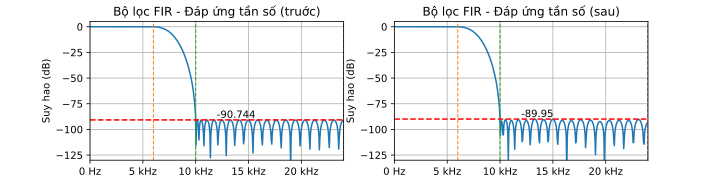
\includegraphics[width=13cm]{Images/Chuong4/hb_fir/fir.png}
    \caption[Kiến trúc các khối điều khiển trong dti\_hb\_fir\_filter]{\bfseries \fontsize{12pt}{0pt}\selectfont Kiến trúc các khối điều khiển trong dti\_hb\_fir\_filter}
    \label{control}
\end{figure}

Hình \ref{pre} và hình \ref{pos} mô tả kiến trúc của phần trước và sau của bộc lọc FIR. Chúng ta có thể thấy chỉ sử dụng 2 bộ cộng - 1 cộng cho các phần tử đối xứng và 1 để cộng dồn các phép toán nhân. Với 2 bộ lọc HB1 và HB2 còn lại sẽ thực hiện tương tự.

Bộ nhân sử dụng ở đây là bộ nhân Booth Wallace, nó là IP số có sẵn của công ty \textbf{Dolphin Technology Việt Nam}.

Với kiến trúc của bộ nhân chung (hình \ref{c_mul}), chúng ta sẽ duyệt các hệ số của các taps sau đó tiến hành nhân ở các thời điểm nhất định. Các hệ số sẽ được lưu ở bộ \textbf{coeff\_lut}, nó được xem là 1 bộ mem, các hệ số sẽ được lưu thứ tự FIR - HB1 - HB2 - HB1 (từ 0 đến 39). Dữ liệu sẽ đưa đưa ra theo địa chỉ \textit{count} tương ứng. Bảng \ref{coeffff} mô tả trình tự sắp đặt dữ liệu trong khối \textbf{coeff\_lut}.

\textbf{dti\_count} hoạt động như một trình tạo địa chỉ và bộ điều khiển của \textbf{dti\_filter\_controller}. Giá trị đếm dùng để chọn hệ số trong bảng tra cứu hệ số bộ lọc (\textbf{dti\_coeff\_lut}).

\paragraph{dti\_filter\_controller}
\begin{figure}[H]
    \centering
    \includegraphics[width=6cm]{Images/Chuong4/hb_fir/control-top.png}
    \caption[Sơ đồ khối của dti\_filter\_controller]{\bfseries \fontsize{12pt}{0pt}\selectfont Sơ đồ khối của dti\_filter\_controller}
    \label{control_t}
\end{figure}
\textbf{dti\_hb\_fir\_filter} chỉ sử dụng 1 bộ nhân nên 2 bộ lọc Half band và bộ lọc FIR buộc phải chia sẻ tài nguyên. \textbf{dti\_filter\_controller} kiểm soát việc sử dụng tài nguyên của các bộ lọc bằng tín hiệu \textbf{select\_filter}.

\begin{figure}[H]
    \centering
    \includegraphics[width=13cm]{Images/Chuong4/hb_fir/control-timing.png}
    \caption[Biểu đồ thời của dti\_filter\_controller]{\bfseries \fontsize{12pt}{0pt}\selectfont Biểu đồ thời  của dti\_filter\_controller}
    \label{control_timing}
\end{figure}
\begin{figure}[H]
    \centering
    \includegraphics[width=14cm]{Images/Chuong4/hb_fir/control-fsm.png}
    \caption[Sơ đồ máy trạng thái hữu hạn của dti\_filter\_controller]{\bfseries \fontsize{12pt}{0pt}\selectfont Sơ đồ máy trạng thái hữu hạn của dti\_filter\_controller}
    \label{control_fsm}
\end{figure}
Sơ đồ chân vào ra mô tả ở hình \ref{control_t}. Các tín hiệu điều khiển hoạt động với chức năng thể hiện ở biểu đồ hình \ref{control_timing}.

Qua sơ đồ hình \ref{control_fsm}, máy trạng thái của bộ có 2 trạng thái:
\begin{itemize}
    \item \textbf{ST\_COUNTING}: bộ đếm tăng giá trị
    \item \textbf{ST\_STOP}: bộ đếm dừng hoạt động
\end{itemize}

Bộ điều khiển có chức năng chia pha cho và chọn thời điểm lấy giá trị đưa vào bộ nhân. Nó cũng điều khiển bộ đếm để lấy giá trị các hệ số của các bộ lọc trong MEM ra. Việc kích hoạt từng bộ lọc sẽ được điều khiển bởi tín hiệu choose\_filter. Vì tần số hệ thống lớn hơn rất nhiều so với điều kiện trong 1 chu kỳ thực hiện phép nhân nên bộ điều khiển phải lấy tín hiệu thực hiện xong tính toán của từng bộ lọc để chờ ở các pha tính toán tiếp theo. 

\begin{table}[H]
\centering
    \caption[Các hệ số của các bộ lọc ứng với từng địa chỉ trong khối coeff\_lut]{\bfseries \fontsize{12pt}{0pt}\selectfont Các hệ số của các bộ lọc ứng với từng địa chỉ trong khối coeff\_lut}
\begin{tabular}{|l|c|c|l|l|c|c|}
\cline{1-3} \cline{5-7}
\multicolumn{1}{|c|}{\textbf{Địa chỉ}} & \textbf{Bộ lọc}       & \textbf{Giá trị} &  & \multicolumn{1}{c|}{\textbf{Địa chỉ}} & \textbf{Bộ lọc}       & \textbf{Giá trị} \\ \cline{1-3} \cline{5-7} 
0                                      & \multirow{10}{*}{FIR} & -96              &  & 10                                    & \multirow{10}{*}{FIR} & 5333             \\ \cline{1-1} \cline{3-3} \cline{5-5} \cline{7-7} 
1 &  & -191  &  & 11 &  & 8971   \\ \cline{1-1} \cline{3-3} \cline{5-5} \cline{7-7} 
2 &  & -12   &  & 12 &  & 4117   \\ \cline{1-1} \cline{3-3} \cline{5-5} \cline{7-7} 
3 &  & 683   &  & 13 &  & -8082  \\ \cline{1-1} \cline{3-3} \cline{5-5} \cline{7-7} 
4 &  & 1560  &  & 14 &  & -17116 \\ \cline{1-1} \cline{3-3} \cline{5-5} \cline{7-7} 
5 &  & 1559  &  & 15 &  & -10866 \\ \cline{1-1} \cline{3-3} \cline{5-5} \cline{7-7} 
6 &  & -220  &  & 16 &  & 10947  \\ \cline{1-1} \cline{3-3} \cline{5-5} \cline{7-7} 
7 &  & -3024 &  & 17 &  & 30749  \\ \cline{1-1} \cline{3-3} \cline{5-5} \cline{7-7} 
8 &  & -4108 &  & 18 &  & 24711  \\ \cline{1-1} \cline{3-3} \cline{5-5} \cline{7-7} 
9 &  & -938  &  & 19 &  & -13469 \\ \cline{1-3} \cline{5-7} 
\end{tabular}
\label{coeffff}
\end{table}
\begin{table}[H]
\centering
\begin{tabular}{|l|c|c|l|l|c|c|}
\cline{1-3} \cline{5-7}
\multicolumn{1}{|c|}{\textbf{Địa chỉ}} & \textbf{Bộ lọc} & \textbf{Giá trị} &  & \multicolumn{1}{c|}{\textbf{Địa chỉ}} & \textbf{Bộ lọc} & \textbf{Giá trị} \\ \cline{1-3} \cline{5-7} 
20 & \multirow{6}{*}{FIR} & -57165 &  & 30 & \multirow{6}{*}{HB2} & 749    \\ \cline{1-1} \cline{3-3} \cline{5-5} \cline{7-7} 
21 &                      & -58588 &  & 31 &                      & -5783  \\ \cline{1-1} \cline{3-3} \cline{5-5} \cline{7-7} 
22 &                      & 15205  &  & 32 &                      & 24260  \\ \cline{1-1} \cline{3-3} \cline{5-5} \cline{7-7} 
23 &                      & 149059 &  & 33 &                      & -78249 \\ \cline{1-1} \cline{3-3} \cline{5-5} \cline{7-7} 
24 &                      & 279548 &  & 34 &                      & 321172 \\ \cline{1-1} \cline{3-3} \cline{5-5} \cline{7-7} 
25 &                      & 333704 &  & 35 &                      & 524288 \\ \cline{1-3} \cline{5-7} 
26 & \multirow{4}{*}{HB1} & 7025   &  & 36 & \multirow{4}{*}{HB1} & 7025   \\ \cline{1-1} \cline{3-3} \cline{5-5} \cline{7-7} 
27 &                      & -53701 &  & 37 &                      & -53701 \\ \cline{1-1} \cline{3-3} \cline{5-5} \cline{7-7} 
28 &                      & 308825 &  & 38 &                      & 308825 \\ \cline{1-1} \cline{3-3} \cline{5-5} \cline{7-7} 
29 &                      & 524288 &  & 39 &                      & 524288 \\ \cline{1-3} \cline{5-7} 
\end{tabular}
\end{table}

\subsection{Kiểm thử}
Việc mô phỏng RTL sẽ được thực hiện trên Mentor Questasim. Tương tự chương 2, chúng ta sẽ trích xuất tín hiệu PDM từ bộ điều chế (thư viện sigmadelta) ra dữ liệu dạng chữ và lưu vào tệp text. Từ đó có thể đưa vào testbench và chạy mô phỏng.
\subsubsection{Cấu trúc testbench}
\begin{figure}[H]
    \centering
    \includegraphics[width=13cm]{Images/Chuong4/tb/tb_top.png}
    \caption[Cấu trúc của testbench]{\bfseries \fontsize{12pt}{0pt}\selectfont  Cấu trúc của testbench}
    \label{tb_top}
\end{figure}

Tín hiệu PDM được đọc từ tệp text thu được bộ điều chế đưa vào thiết kế với tần số lấy mẫu của PDM (2304 kHz). Dữ liệu PCM thu được đầu ra với tần số mẫu là 48 kHz đưa ghi vào tệp text. Từ tệp đó chúng ta sẽ so sánh với kết quả tính toán bằng phần mềm sử dụng ngôn ngữ \textbf{python} (hình \ref{tb_top}). Việc so sánh sẽ đựa vào biểu đồ mật độ phổ công suất và tín hiệu ở miền thời gian.

\subsubsection{Kết quả mô phỏng}
\paragraph{Tín hiệu nhiều thành phần sin}
Như ở trong \hyperref[chuong3]{chương 3}, tín hiệu 3 thành phần gồm 3 sóng sin có tần số lần lượt 4 kHz, 13 kHz, 22 kHz như phương trình \ref{3sin2}.
\begin{equation} \label{3sin2}
    x(t) = \frac{0.4}{3} (sin(2\pi \times 4000\times t) + sin(2\pi \times 13000\times t) + sin(2\pi \times 22000\times t))
\end{equation}

Ban đầu chúng ta sẽ cấu hình độ rộng của PCM là 20.

Hình \ref{sin_1} và \ref{sin_1_1} miêu tả biểu đồ thời gian của tín hiệu PCM sau mô phỏng của cả phần cứng và phần mềm. Ở miền này hầu như chúng ta không thể nhận ra sự khác biệt. Các thần phần tần số 13 kHz, 22 kHz đã được loại bỏ chỉ còn sóng sin của tần số 4 kHz tồn tại.

Để kết luận một cách rõ ràng hơn, chúng sẽ xem xét miền tần số của 2 tín hiệu. Hình \ref{psd_sin_1}, hình \ref{psd_sin_1_1} mô tả biểu đồ phổ mật độ công suất của 2 tín hiệu trên. Vì 2 thành phần tần số 13 kHz và 22 kHz nằm trong dải dừng (thành phần bị loại bỏ) và nó có biên độ bằng thành phần tần số 4 kHz (nằm trong dải thông), chúng ta có thể lấy độ chênh lệch của các thành phần tần số này trong miền tần số để kết luận về độ suy hao của dải dừng.

\begin{figure}[H]
    \centering
    \includegraphics[width=14cm]{Images/Chuong4/tb/sim/sin_1.png}
    \caption[Miền thời gian của tín hiệu mô phỏng bằng phần cứng với độ rộng PCM là 20]{\bfseries \fontsize{12pt}{0pt}\selectfont Miền thời gian của tín hiệu mô phỏng bằng phần cứng với độ rộng PCM là 20}
    \label{sin_1}
\end{figure}

\begin{figure}[H]
    \centering
    \includegraphics[width=14cm]{Images/Chuong4/tb/sim/sin_1_1.png}
    \caption[Miền thời gian của tín hiệu mô phỏng trên phần mềm với độ rộng PCM là 20]{\bfseries \fontsize{12pt}{0pt}\selectfont Miền thời gian của tín hiệu mô phỏng trên phần mềm}
    \label{sin_1_1}
\end{figure}

\begin{figure}[H]
    \centering
    \includegraphics[width=14cm]{Images/Chuong4/tb/sim/psd_sin_1.png}
    \caption[Phổ của tín hiệu mô phỏng bằng phần cứng với độ rộng PCM là 20]{\bfseries \fontsize{12pt}{0pt}\selectfont  Phổ của tín hiệu mô phỏng bằng phần cứng với độ rộng PCM là 20}
    \label{psd_sin_1}
\end{figure}

\begin{figure}[H]
    \centering
    \includegraphics[width=14cm]{Images/Chuong4/tb/sim/psd_sin_1_1.png}
    \caption[ Phổ của tín hiệu mô phỏng bằng phần mềm]{\bfseries \fontsize{12pt}{0pt}\selectfont  Phổ của tín hiệu mô phỏng bằng phần mềm }
    \label{psd_sin_1_1}
\end{figure}

Chúng ta có thể dễ dàng nhận thấy (hình \ref{psd_sin_1}, \ref{psd_sin_1_1}), độ suy hao giảm khoảng 8 dB ở thiết kế phần cứng so với mô phỏng phần mềm. Tuy nhiên nó vẫn nằm gần khoảng giá trị 89 dB, điều này đã đáp ứng được yêu cầu thiết kế của dải dừng. Tuy nhiên ở các thành phần tín hiệu nhiễu trong dải dừng có vẻ tăng đột ngột và độ chính xác so với phần mềm không cao.

Ở dải thông, thiết kế đã đáp ứng được trong khoảng tần số 0 - 6kHz, tuy nhiên có 1 số thành phần tần số khác có độ chính xác không cao so với phần mềm. Ở tần số 6 kHz đã có sự chuyển đến tần số 10 kHz, vì vậy đã đáp ứng được yêu cầu dải chuyển tiếp.

Từ điểm 10 kHz trở đi dải dừng ổn định nhưng với độ suy hao cao hơn nhiều so với độ suy hao bằng mô phỏng phần mềm.

Những sai số đó gây ra bởi độ rộng của PCM lấy mẫu, số bit bị cắt bỏ sau mỗi tầng lọc để giảm tài nguyên. Để kiểm tra về tác nhân gây sai số, chúng ta tăng độ rộng của PCM lên 24 bit và chạy lại mô phỏng.

Về biểu đồ thời gian (hình \ref{sin_2}) không có gì khác biệt so với mô phỏng với phần mềm và trường hợp độ rộng PCM là 20 bit. Chúng ta sẽ xem xét rõ hơn ở miền tần số.

Hình \ref{psd_sin_2} mô tả biều đồ mật độ công suất của tín hiệu PCM đầu ra với trường hợp độ rộng bit là 24 bit. Độ suy hao đã bám sát giá trị 89 dB với độ chênh lệch là 0.077 dB. Các thành phần tín hiệu ở các tần số khác được hiện thị rõ ràng hơn so với trường hợp 20 bit. Dải chuyển tiếp có độ sâu hơn. Hình dạng của mật độ công suất đã gần như giống với tín hiệu được mô phỏng bằng phần mềm.

Chúng ta có thể tăng độ rộng bit của PCM lên để đạt được các thông số tốt hơn và giống với phần mềm. Tuy nhiên điều đó gây tốn tài nguyên. Với số bit là 24 thì đã hoàn toàn đáp ứng được với thiết kế. Thật vậy, ở dạng âm thanh chất lượng cao thì độ rộng của PCM thường là 24.

\begin{figure}[H]
    \centering
    \includegraphics[width=14cm]{Images/Chuong4/tb/sim/sin_2.png}
    \caption[Miền thời gian của tín hiệu mô phỏng trên phần mềm với độ rộng PCM là 24]{\bfseries \fontsize{12pt}{0pt}\selectfont  Miền thời gian của tín hiệu mô phỏng trên phần mềm với độ rộng PCM là 24}
    \label{sin_2}
\end{figure}

\begin{figure}[H]
    \centering
    \includegraphics[width=14cm]{Images/Chuong4/tb/sim/psd_sin_2.png}
    \caption[Phổ của tín hiệu mô phỏng bằng phần cứng với độ rộng PCM là 24]{\bfseries \fontsize{12pt}{0pt}\selectfont  Phổ của tín hiệu mô phỏng bằng phần cứng với độ rộng PCM là 24 }
    \label{psd_sin_2}
\end{figure}

\paragraph{Tín hiệu từ tệp âm thanh có sẵn}

Có một cách khác để kiểm tra tín hiệu âm thanh thu được thực tế hơn đó là nghe bằng tai. Khi được số hóa, tín hiệu âm thanh sẽ được lưu trữ dưới dạng tệp ".wav, .mp3, \ldots" Từ các tệp này chúng ta có thể nghe lại ở mọi thiết bị và mọi thời điểm. Với tín hiệu chất lượng cao - độ phân dải là 24 bit, tần số lấy mẫu là 48 kHz nó sẽ được lưu dưới dạng tệp wav.

Vận dụng các đặc điểm đó, chúng ta sẽ tiến hành đọc dữ liệu ở tệp và sau đó điều chế Sigma-Delta để thu được tín hiệu PDM. Tín hiệu này sau đó sẽ được đưa vào testbench để chạy mô phỏng.

Tiến hành mô phỏng với tệp nhạc có cả nhạc nền và giọng hát.

\begin{figure}[H]
    \centering
    \includegraphics[width=14cm]{Images/Chuong4/tb/wav/vldd2_2.png}
    \caption[Biểu đồ miền thời gian của âm thanh gốc]{\bfseries \fontsize{12pt}{0pt}\selectfont Biểu đồ miền thời gian của âm thanh gốc}
    \label{vldd2_2}
\end{figure}

Hình \ref{vldd2_2} là biều đồ biểu thị 1 phần nhỏ tín hiệu gốc của tệp đề cập ở trên. Sau khi đi qua bộ chuyển đổi bằng phần cứng (hình \ref{vldd2_0}) và bộ chuyển đổi sử dụng tính toán bằng phần mềm (hình \ref{vldd2_1}), ta thấy được sự khác biệt giữa các biểu đồ. Tín hiệu gốc dường nhưng đã mất đi một phần tín hiệu nào đó khiến nó bị biến dạng. Tuy nhiên biểu đồ giữa mô phỏng bằng phần cứng và phần mềm lại được xem là giống nhau. Để hiểu rõ chi tiết hơn, chúng ta nên xem các tín hiệu trên biểu diễn trên miền tần số.

\begin{figure}[H]
    \centering
    \includegraphics[width=14cm]{Images/Chuong4/tb/wav/vldd2_0.png}
    \caption[Biểu đồ miền thời gian của âm thanh sau khi đi qua bộ chuyển đổi]{\bfseries \fontsize{12pt}{0pt}\selectfont  Biểu đồ miền thời gian của âm thanh sau khi đi qua bộ chuyển đổi }
    \label{vldd2_0}
\end{figure}

\begin{figure}[H]
    \centering
    \includegraphics[width=14cm]{Images/Chuong4/tb/wav/vldd2_1.png}
    \caption[Biểu đồ miền thời gian của âm thanh sau sau khi chuyển đổi bằng phần mềm]{\bfseries \fontsize{12pt}{0pt}\selectfont  Biểu đồ miền thời gian của âm thanh sau sau khi chuyển đổi bằng phần mềm}
    \label{vldd2_1}
\end{figure}

\begin{figure}[H]
    \centering
    \includegraphics[width=14cm]{Images/Chuong4/tb/wav/vldd2_psd_2.png}
    \caption[Biểu đồ phổ của tín hiệu âm thanh gốc]{\bfseries \fontsize{12pt}{0pt}\selectfont Biểu đồ phổ của tín hiệu âm thanh gốc}
    \label{vldd2_psd_2}
\end{figure}

Hình \ref{vldd2_psd_2} mô tả mật độ phổ công suất của tín hiệu gốc. Chúng ta có thể thấy tín hiệu sẽ có đủ dải từ 0 - 24 kHz. Sau khi đưa qua mô phỏng tín hiệu đã bị lọc bỏ hết thành phần từ 6 - 24 kHz, điều này khiến ở miền thời gian tín hiệu sau khi chuyển đổi bị biến dạng. Hình \ref{vldd2_psd_0} và \ref{vldd2_psd_1} lần lượt là phổ của tín hiệu âm thanh sau khi đi qua mô phỏng phần cứng và phần mềm. Chúng ta có thể thấy ở dải thông, các thành phần tín hiệu ở dải tần số khá là tương tự nhau. Nó chỉ khác biệt là khi chuyển xuống dải dừng, độ suy hao của phần cứng sẽ chênh lệch với phần mềm khoảng 9 dB. Như đã đề cập ở phần trước thì độ chênh lệnh này không ảnh hưởng so với yêu cầu thiết kế là 89 dB.

Khi nghe lại 2 tệp âm thanh trước và sau khi chuyển đổi bằng phần cứng, chúng ta có nhận xét sau đây: âm thanh sau khi chuyển đổi dường đi mất đi sự chi tiết, tươi sáng và sắc bén. 

Vì bộ chuyển đổi sẽ loại bỏ đi các thành phần ở tần số 6 - 24 kHz, thật trùng hợp vì đây cũng là dải tần số \textbf{Treble} (6 kHz - 20 kHz) của âm thanh. Mà dải này đảm nhận vai trò tăng độ chi tiết cho âm thanh, do đó tín hiệu nghe được bị mất cảm xúc cũng là điều hoàn toàn đúng.

\begin{figure}[H]
    \centering
    \includegraphics[width=14cm]{Images/Chuong4/tb/wav/vldd2_psd_0.png}
    \caption[Biểu đồ phổ của âm thanh sau khi chuyển đổi bằng phần cứng]{\bfseries \fontsize{12pt}{0pt}\selectfont  Biểu đồ phổ của âm thanh sau khi chuyển đổi bằng phần cứng}
    \label{vldd2_psd_0}
\end{figure}

\begin{figure}[H]
    \centering
    \includegraphics[width=14cm]{Images/Chuong4/tb/wav/vldd2_psd_1.png}
    \caption[Biểu đồ phổ của âm thanh sau sau khi chuyển đổi bằng phần mềm]{\bfseries \fontsize{12pt}{0pt}\selectfont  Biểu đồ phổ của âm thanh sau sau khi chuyển đổi bằng phần mềm}
    \label{vldd2_psd_1}
\end{figure}

\subsection{Kết luận chương}

\hyperref[chuong4]{Chương 5} đã giải quyết được vấn đề thiết kế bộ chuyển đổi nhiều giai đoạn với ngôn ngữ mô tả phần cứng SystemVerilog. Kết quả kiểm thử cho thấy thiết kế có sai số so với việc tính toán bằng phần mềm nhưng vẫn đáp ứng được với các yêu cầu thiết kế đặt ra. Trong chương tiếp theo, thiết kế này sẽ được tổng hợp và triển khai lên FPGA để kiếm chứng tính đúng đắn trong điều kiện thực tế.

\newpage
% \phantomsection\addcontentsline{toc}{section}{\numberline {}CHƯƠNG 5. TỔNG HỢP VÀ TRIỂN KHAI TRÊN FPGA}
\section*{CHƯƠNG 5. TỔNG HỢP VÀ TRIỂN KHAI TRÊN FPGA} \label{chuong5}
\setcounter{section}{5}
\setcounter{subsection}{0}
\setcounter{figure}{0}
\setcounter{table}{0}
Chương này sẽ trình bày chi tiết về quá trình sử dụng Design Compiler để tổng hợp mạch điện tử số, từ các bước chuẩn bị thiết kế đến các bước tối ưu hóa và đánh giá mạch. Cuối cùng, để đảm bảo thiết kế chạy ổn định trong thiết bị thực tế thì chúng ta triển khai hệ thống đã được xây dựng ở chương trước lên kit FPGA, ở đây sẽ sử dụng kit Zedboard của hãng Xilinx.

\subsection{Tổng hợp và phân tích timing}
Design Compiler là một công cụ tổng hợp logic, cho phép tổng hợp các mạch điện tử số từ ngôn ngữ Verilog hoặc VHDL sang mạch RTL (Register-Transfer Level) và sau đó là mạch gate-level để có thể được triển khai trên ASIC hoặc FPGA. 

Thiết kế được tổng hợp với thư viện standard cell \textbf{dti\_tm28hpcp\_l30\_stdcells\_7t\_rev1p0p1} của \textbf{Dolphin Technology VietNam Center} bằng phần mềm \textbf{Design Compiler}. Chúng ta có các báo cáo sau:
\subsubsection{Kết quả phân tích timing}
Đây là phần cần quan tâm nhất sau khi tổng hợp, vì các quy định về mặt timing là 
buộc phải tuân thủ.


\begin{table}[H]
\centering
\caption[Báo cáo timing của thiết kế]{\bfseries \fontsize{12pt}{0pt}\selectfont Báo cáo timing của thiết kế}
\begin{tabular}{|l|l|}
\hline
\multicolumn{1}{|c|}{\textbf{Thông tin}} & \multicolumn{1}{c|}{{\begin{tabular}[c]{@{}c@{}}\textbf{Giá trị}\\ (ns)\end{tabular}}} \\ \hline
Chu kỳ Critical Path Clk & 50.00000 \\ \hline
Critical Path Slack & 35.52476 \\ \hline
Critical Path Length & 4.43226 \\ \hline
\end{tabular}
\label{syn_t}
\end{table}

% \begin{figure}[H]
%     \centering
%     \includegraphics[width=12cm]{Images/Chuong5/syn/timing.png}
%     \caption[Báo cáo timing của thiết kế]{\bfseries \fontsize{12pt}{0pt}\selectfont Báo cáo timing của thiết kế}
%     \label{syn_t}
% \end{figure}

Với yêu cầu của bộ thiết là tần số chạy không cao (9216 kHz) thì về mặt timing không có gì cần phải quan tâm vì nó chắc chắn sẽ thỏa mãn. Thật vậy:
Đưa các ràng buộc về timing như sau:
\begin{itemize}
    \item Tần số tổng hợp: 20 MHz ($>$ 9216 kHz)
    \item Độ trễ đầu vào: cao nhất là 0.4 chu kỳ clock
    \item Độ trễ đầu đầu ra: cao nhất là 0.4 chu kỳ clock
\end{itemize}

Các thông số input delay và output delay được xác định khi ta ghép khối PDM2PCM 
với các khối khác trong hệ thống. Các khối khác chưa được hoàn thiện nên ta đặt các ràng buộc mang tính tương đối.

Báo cáo về mặt timing sẽ được mô tả ở bảng \ref{syn_t}. Ta thấy slack của critical path (đường có trễ cao nhất) đang dương rất lớn, từ đó có thể kết luận thiết kế thỏa mãn về timing.
\subsubsection{Tài nguyên sử dụng}

\begin{table}[H]
\centering
    \caption[Các báo cáo về mặt diện tích của thiết kế]{\bfseries \fontsize{12pt}{0pt}\selectfont Các báo cáo về mặt diện tích của thiết kế}
\begin{tabular}{|l|l|}
\hline
\multicolumn{1}{|c|}{\textbf{Thông tin}} &
  \multicolumn{1}{c|}{\textbf{\begin{tabular}[c]{@{}c@{}}Thông số\\ ($\mu m^2$)\end{tabular}}} \\ \hline
\begin{tabular}[c]{@{}l@{}}Diện tích phần tổ hợp\\ (Combinational area)\end{tabular}    & 1803.689998 \\ \hline
\begin{tabular}[c]{@{}l@{}}Diện tích phần buffer/inverter\\ (Buf/Inv area)\end{tabular} & 102.997997  \\ \hline
\begin{tabular}[c]{@{}l@{}}Diện tích phần không phải mạch tổ hợp\\ (Noncombinational area)\end{tabular} &
  3661.475934 \\ \hline
\begin{tabular}[c]{@{}l@{}}Diện tích phần hộp đen\\ (Macro/Black Box area)\end{tabular} & 0.000000    \\ \hline
Tổng cộng                                                                               & 5465.165932 \\ \hline
\end{tabular}
    \label{area}
    \end{table}

Bảng \ref{cell}, \ref{area} mô tả về mặt vật lý, nó chỉ rõ ra các số lượng port, net, các cell combinational và sequential. Từ đó đưa ra tổng diện tích của thiết kế.
Nhận thấy tổng diện tích 5465.165932 ($\mu m^2$) là trung bình ở mức chấp nhận được với những IP chuyển đổi.
\begin{table}[H]
\centering
    \caption[Các báo cáo về mặt số lượng phần tử của thiết kế]{\bfseries \fontsize{12pt}{0pt}\selectfont Các báo cáo về mặt số lượng phần tử của thiết kế}
    \begin{tabular}{|lc|l|}
\hline
\multicolumn{2}{|c|}{\textbf{Thông tin}}                    & \multicolumn{1}{c|}{\textbf{Số lượng}} \\ \hline
\multicolumn{2}{|l|}{Số port}                               & 29                                     \\ \hline
\multicolumn{2}{|l|}{Số lượng dây (nets)}                   & 6002                                   \\ \hline
\multicolumn{1}{|l|}{\multirow{2}{*}{Số cell}}   & Tuần tự  & 1664                                   \\ \cline{2-3} 
\multicolumn{1}{|l|}{}                           & Tổ hợp   & 4276                                   \\ \hline
\multicolumn{2}{|l|}{Số lượng hộp đen (macros/black boxes)} & 0                                      \\ \hline
\multicolumn{2}{|l|}{Số buffer/inveter}                     & 525                                    \\ \hline
\end{tabular}
    \label{cell}
    \end{table}

\subsubsection{Công suất}
% \begin{figure}[H]
%     \centering
%     \includegraphics[width=14cm]{Images/Chuong5/syn/power.png}
%     \caption[Báo cáo công suất của thiết kế]{\bfseries \fontsize{12pt}{0pt}\selectfont Báo cáo công suất của thiết kế}
%     \label{syn_power}
% \end{figure}



Báo cáo về mặt công suất chỉ ra các thông số về mặt tiêu thụ năng nương, như năng 
lượng chuyển mạch, dòng dò, năng lượng bản thân cho các cell hoạt động. Báo cáo được mô tả như bảng \ref{syn_power}.
\begin{table}[H]
\centering
\caption[Báo cáo công suất của thiết kế]{\bfseries \fontsize{12pt}{0pt}\selectfont Báo cáo công suất của thiết kế}
\begin{tabular}{|l|l|}
\hline
\multicolumn{1}{|c|}{\textbf{Thông tin}} & \multicolumn{1}{c|}{\textbf{Giá trị}} \\ \hline
Internal Power & 7.52089e-02 (mW) \\ \hline
Switching Power & 1.97545e-03 (mW) \\ \hline
Leakage Power & 332.52689 (nW) \\ \hline
Tổng cộng & 7.75168e-02 (mW) \\ \hline
\end{tabular}
\label{syn_power}
\end{table}
\subsection{Triển khai thiết kế xuống FPGA}
Sau khi hoàn thành mô phỏng và tổng hợp, đảm bảo thiết kế hoạt động đúng chức 
năng yêu cầu. Để đảm bảo thiết kế hoạt động ổn định trong các thiết bị thực tế thì chúng ta sẽ triển khai thiết kế xuống FPGA.

\textbf{Giới thiệu về kit phát triển Zedboard} (hình \ref{zedboard}):

Zedboard được thiết kế trên nền tảng của một vi xử lý ARM Cortex-A9 MPCore lõi kép của Xilinx, với các tính năng khác như bộ nhớ DDR3, kết nối Ethernet, USB và các cổng giao tiếp khác như PMOD và FMC. Zedboard cũng được trang bị một FPGA Xilinx 7 series để cho phép người dùng tùy chỉnh phần cứng và thiết kế các hệ thống phức tạp.

\begin{figure}[H]
    \centering
    \includegraphics[width=12cm]{Images/Chuong5/fpga/zedboard.jpg}
    \caption[Kit ZedBoard]{\bfseries \fontsize{12pt}{0pt}\selectfont Kit ZedBoard}
    \label{zedboard}
\end{figure}

Zedboard được thiết kế trên nền tảng của một vi xử lý ARM Cortex-A9 MPCore lõi kép của Xilinx, với các tính năng khác như bộ nhớ DDR3, kết nối Ethernet, USB và các cổng giao tiếp khác như PMOD và FMC. 


Kit phát triển Zedboard được thiết kế để hỗ trợ các phần mềm như Xilinx SDK và Vivado Design Suite, cho phép người dùng thiết kế phần cứng và phần mềm cùng một lúc trên một nền tảng. Điều này giúp tăng hiệu suất và tối ưu hóa thiết kế phần cứng và phần mềm.

Với các tính năng và khả năng linh hoạt của nó, Zedboard là một công cụ hữu ích cho các kỹ sư và nhà phát triển trong việc phát triển các hệ thống nhúng phức tạp và đòi hỏi sự tùy chỉnh cao.



\subsubsection{Thiết kế bộ bao để triển khai trên hệ thống SOC} \label{wrapper_cha}

Để triển khai thiết kế lên hệ thống SOC (System On Chip), chúng ta cần sử dụng một bộ điều khiển để xử lý và đọc dữ liệu của đầu ra PCM, sau đó lưu vào một vùng nhớ có địa chỉ cố định. Từ địa chỉ đó vi xử lý mới có thể đọc dữ liệu về và làm những bước tiếp theo. Hình \ref{wrapper} mô tả kiến trúc của bộ bao (pdm2pcm\_warpper) nó sử dụng chuẩn giao tiếp APB (Advanced Peripheral Bus) -  1 chuẩn giao tiếp rất phổ biến trong hệ thống SOC dùng để giao tiếp với ngoại vi.

\begin{figure}[H]
    \centering
    \includegraphics[width=13cm]{Images/Chuong5/fpga/wrapper.png}
    \caption[Sơ đồ khối của bộ pdm2pcm\_warpper]{\bfseries \fontsize{12pt}{0pt}\selectfont Sơ đồ khối của bộ pdm2pcm\_warpper}
    \label{wrapper}
\end{figure}

Khối \textbf{register\_block} đóng vai trò trung chuyển dữ liệu từ pdm2pcm lên vi xử lý. Nó lưu 2 giá trị PCM đầu ra và trạng thái trống của bộ đệm. Nó có cấu trúc như hình \ref{bit}. Thiết kế này chỉ lấy 16bit PCM và sẽ được phát trên 2 kênh trái và phải của loa.

\begin{figure}[H]
    \centering
    \includegraphics[width=9cm]{Images/Chuong5/fpga/bit.png}
    \caption[Sơ đồ khối của bộ pdm2pcm\_warpper]{\bfseries \fontsize{12pt}{0pt}\selectfont Sơ đồ khối của bộ pdm2pcm\_warpper}
    \label{bit}
\end{figure}

Lúc này vi xử lý có thể biết lúc nào có thể đọc (có dữ liệu) thông qua thanh ghi rd\_empty, khi đó dữ liệu đã có sẵn trên thanh ghi pcm\_data và có thế đọc. Các giá trị trong thanh ghi sẽ được cập nhật liên tục với tần số của hệ thống chính.

Vì thiết kế sử dụng tần số khác với tần số của hệ thống (2 miền tần số) sẽ dẫn đến thất lạc dữ liệu ở 1 số thời điểm, điều đó gây mất chính xác của hệ thống. Để  sai sót này, chúng ta sẽ chèn 1 bộ đệm không đồng bộ để đồng bộ hai miền tần số. Tất cả các dữ liệu đầu ra PCM sẽ được ghi liên tục vào \textbf{async\_fifo} và tất nhiên lúc fifo đầy sẽ dừng. Bộ fifo sẽ nhận được tín hiệu đọc dữ liệu ra thông qua các sự kiện đọc từ vi xử lý thông qua bus APB, lúc này trên \textbf{register\_block} sẽ cập nhật giá trị mới. Tín hiệu rd\_empty cũng báo cho hệ thống là bộ lọc đang hay không có dữ liệu, điều này là hết sức cần thiết để thông báo cho vi xử lý biến lúc nào cần lấy dữ liệu.

\subsubsection{Ý tưởng thiết kế}

Tín hiệu PDM sẽ được tạo ra từ micro MEMS được bán trên thị trường. Ý tưởng ở đây là hệ thống đọc tín hiệu từ micro và sau đó phát qua loa một trong thời gian thực.
Ý tưởng mô tả như hình hình \ref{pinouts}.
\begin{figure}[H]
    \centering
    \includegraphics[width=14cm]{Images/Chuong5/fpga/top.png}
    \caption[Sơ đồ ý tưởng của thiết kế]{\bfseries \fontsize{12pt}{0pt}\selectfont Sơ đồ ý tưởng của thiết kế}
    \label{pinouts}
\end{figure}

Trên kit Zedboard đã có sẵn bộ I2S Audio CODEC - ADAU1761, nó sẽ được tận dụng để phát âm thanh ra loa. Chúng ta sẽ sử dụng thêm bộ I2S master để chuyển đổi tín hiệu PCM thành I2S sau đó dùng ADAU1761 để chuyển đổi sang tín hiệu tương tự và phát ra loa. Điều đáng chú ý ở đây, ADAU1761 được cấu hình các thông số thông qua giao tiếp SPI hoặc I2C vì vậy chúng ta sẽ sử dụng thêm bộ I2C master để làm việc này. Sơ đồ khối chi tiết và cách làm việc sẽ được trình bày ở mục tiếp theo.

Để kiểm soát toàn bộ các quá trình gửi và nhận dữ liệu từ PC, bộ xử lí MicroBlaze được sử dụng để làm trung gian điều phối quá trình gửi và nhận dữ liệu

Hình \ref{adau} mô tả kiến trúc bên trong của IC ADAU1761. Đầu ra âm thanh của nó có 2 kênh (stereo) được xử lý hoàn toàn riêng biệt với nhau. Bộ \textbf{PLL} để tạo ra các tần số cần dùng. Khối \textbf{Serial Data} thực chất là I2S slave, nó thu nhận tín hiệu sau đó gửi đến các bộ lọc để đưa tín hiệu ra các kênh. Việc cấu hình thiết bị sẽ do bộ \textbf{I2S/SPI Control Port} xử lý.

\begin{figure}[H]
    \centering
    \includegraphics[width=14cm]{Images/Chuong5/fpga/adau.png}
    \caption[Sơ đồ khối của ADAU1761]{\bfseries \fontsize{12pt}{0pt}\selectfont Sơ đồ khối của ADAU176}
    \label{adau}
\end{figure}



\subsubsection{Triển khai trên trên phần mềm Vivado}

Kit phát triển Zedboard được thiết kế để hỗ trợ các phần mềm như Xilinx SDK và Vivado Design Suite, cho phép người dùng thiết kế phần cứng và phần mềm cùng một lúc trên một nền tảng,  giúp tăng hiệu suất và tối ưu hóa thiết kế phần cứng và phần mềm.

Do sử dụng kit trong đề tài này là Zedboard đồng nghĩa với việc chúng ta phải thực hiện tất cả các quá trình trên phần mềm Vivado - một nền tảng phát triển của \textbf{Xilinx}.
Quy trình thực hiện sẽ bao gồm các bước như sau:
\begin{enumerate}
    \item Tạo dự án: chọn kit sử dụng, ...
    \item Pakage tất cả các IP: I2S, I2C, pdm2pcm\_wrapper
    \item Viết driver code bằng ngôn ngữ C
    \item Mô phỏng thiết kế qua phần mềm QuestaSim
    \item Gán chân vào ra ứng với các cổng trên kit
    \item Tổng hợp
    \item Triển khai thiết kế
    \item Tạo bitstream
    \item Nạp xuống kit
\end{enumerate}



\paragraph{Thiết kế block design}

\begin{figure}[H]
    \centering
    \includegraphics[width=15cm]{Images/Chuong5/fpga/block_design_1.png}
    \caption[Block design của hệ thống]{\bfseries \fontsize{12pt}{0pt}\selectfont Block design của hệ thống}
    \label{bd1}
\end{figure}

\begin{figure}[H]
    \centering
    \includegraphics[width=15cm]{Images/Chuong5/fpga/block_design_2.png}
    \caption[Block design của hệ thống (tiếp)]{\bfseries \fontsize{12pt}{0pt}\selectfont Block design của hệ thống (tiếp)}
    \label{bd2}
\end{figure}
Hình \ref{bd1}, \ref{bd2} mô tả block design của hệ thống. Với bộ não trung tâm là vi xử lý MicroBlaze (\textbf{microblaze\_0}) đảm nhận vai trò đọc ghi và xử lý dữ liệu. Bộ Clock Wizard (\textbf{clk\_wir\_0}) thực hiện tạo ra các tần số mong muốn, ở đây ta có top\_clk ứng với tần số 50 MHz cung cấp cho toàn bộ hệ thống, i2s\_clk là tần số cấp cho bộ I2S với giá trị 36.864 MHz và tần số cấp cho bộ lọc filter\_clk là 9.216 Mhz.

 Khối \textbf{axi\_interconnect\_0} đảm nhận việc ánh xạ một thiết bị master AXI ra nhiều slave AXI. Hệ thống sử dụng chuẩn AXI để làm interconnect (AXI Interconnect), bộ này quản lý (phân địa chỉ) tất cả các ngoại vi. Nó được xem là bộ điều khiển sao cho việc truy xuất dữ liệu đúng với yêu cầu từ vi xử lý.

Khối \textbf{axi\_apb\_bridge}, \textbf{microblaze\_0} giao tiếp theo chuẩn AXI còn các lõi 
thiết kế thì giao tiếp bằng chuẩn APB nên cần một khối có thể chuyển đổi các chuẩn 
giao tiếp này
% \newpage


Bộ \textbf{AXI UART 16550} dùng để truyền và nhận dữ liệu thông qua chuẩn UART. Nó là cổng trung gian để kết nối với PC, từ đây PC có thể đọc được dữ liệu từ hệ thống, thông thường sẽ đi kèm với câu lênh \textit{printf(char*)}.

Bộ \textbf{dti\_pdm2pcm\_apb\_0} là bộ bao đã được thiết kế ở mục \ref{wrapper_cha}. Nó sử dụng chuẩn APB thực hiện đọc ghi dữ liệu, nên để kết nối với vi xử lý chúng ta cần thêm 1 bộ cầu nối để dùng chuẩn AXI.

\textbf{DTI I2S Controller IP} và \textbf{DTI I2C Controller IP} lần lượt là I2S master và I2C master, tất cả các IP đều được do công ty \textbf{Dolphin Tecnology VietNam Center} phát triển. Chúng sử dụng giao thức APB để cấu hình cũng như điều khiển truyền dữ liệu.
\begin{table}[H]
\centering
    \caption[Sắp xếp địa chỉ trong block design]{\bfseries \fontsize{12pt}{0pt}\selectfont Sắp xếp địa chỉ trong block design}
    \begin{tabular}{|lllllll}
\hline
\multicolumn{2}{|c|}{\textbf{Tên}} &
  \multicolumn{1}{c|}{\textbf{\begin{tabular}[c]{@{}c@{}}Giao diện \\ Slave\end{tabular}}} &
  \multicolumn{1}{c|}{\textbf{Kiểu}} &
  \multicolumn{1}{c|}{\textbf{Địa chỉ offset}} &
  \multicolumn{1}{c|}{\textbf{\begin{tabular}[c]{@{}c@{}}Phạm \\ vi\end{tabular}}} &
  \multicolumn{1}{c|}{\textbf{Địa chỉ cao nhất}} \\ \hline
\multicolumn{7}{|l}{Dữ liệu - Data (32 address bits : 4G)} \\ \hline
 &
  \multicolumn{1}{l|}{GPIO} &
  \multicolumn{1}{l|}{S\_AXI} &
  \multicolumn{1}{l|}{Reg} &
  \multicolumn{1}{l|}{0x4000\_0000} &
  \multicolumn{1}{l|}{64K} &
  \multicolumn{1}{l|}{0x4000\_FFFF} \\ \hline
 &
  \multicolumn{1}{l|}{UART 16550} &
  \multicolumn{1}{l|}{S\_AXI} &
  \multicolumn{1}{l|}{Reg} &
  \multicolumn{1}{l|}{0x44A0\_0000} &
  \multicolumn{1}{l|}{64K} &
  \multicolumn{1}{l|}{0x44A0\_FFFF} \\ \hline
 &
  \multicolumn{1}{l|}{Local Memory} &
  \multicolumn{1}{l|}{SLMB} &
  \multicolumn{1}{l|}{Mem} &
  \multicolumn{1}{l|}{0x0000\_0000} &
  \multicolumn{1}{l|}{32K} &
  \multicolumn{1}{l|}{0x0000\_7FFF} \\ \hline
 &
  \multicolumn{1}{l|}{I2C Controller} &
  \multicolumn{1}{l|}{S\_APB} &
  \multicolumn{1}{l|}{Reg} &
  \multicolumn{1}{l|}{0x44A2\_0000} &
  \multicolumn{1}{l|}{64K} &
  \multicolumn{1}{l|}{0x44A2\_FFFF} \\ \hline
 &
  \multicolumn{1}{l|}{I2S Controller} &
  \multicolumn{1}{l|}{S\_APB} &
  \multicolumn{1}{l|}{Reg} &
  \multicolumn{1}{l|}{0x44A3\_0000} &
  \multicolumn{1}{l|}{64K} &
  \multicolumn{1}{l|}{0x44A3\_FFFF} \\ \hline
 &
  \multicolumn{1}{l|}{PDM2PCM} &
  \multicolumn{1}{l|}{\begin{tabular}[c]{@{}l@{}}PDM2PCM\\ \_APB\_v2\end{tabular}} &
  \multicolumn{1}{l|}{Reg} &
  \multicolumn{1}{l|}{0x44A4\_0000} &
  \multicolumn{1}{l|}{64K} &
  \multicolumn{1}{l|}{0x44A4\_FFFF} \\ \hline
\multicolumn{7}{|l}{Lệnh - Instruction (32 address bits : 4G)} \\ \hline
 &
  \multicolumn{1}{l|}{Local Memory} &
  \multicolumn{1}{l|}{SLMB} &
  \multicolumn{1}{l|}{Mem} &
  \multicolumn{1}{l|}{0x0000\_0000} &
  \multicolumn{1}{l|}{32K} &
  \multicolumn{1}{l|}{0x0000\_7FFF} \\ \hline
\end{tabular}
\label{address}
\end{table}
Để báo hiệu dữ liệu đã có sự thay đổi, ở đây có sử dụng thêm bộ \textbf{AXI GPIO} dùng để nháy các đèn led trên kit.

Địa chỉ của từng Slave trong thiết kế được mô tả ở bảng \ref{address}.



\paragraph{Triển khai driver code} \label{code}
Hình \ref{flow_chart} mô tả lưu đồ thuật toán của hệ thống. Trên các IP I2C, I2S, PDM2PCM đều có khối thanh ghi, ban đầu chúng ta phải gán các giá trị mặc định cho nó. Việc cấu hình các IP sẽ thực hiện sau đó, có những điều cần chú ý như sau:
\begin{itemize}
    \item \textbf{I2C}: Với ADAU1761, khi sử dụng cách cấu hình bằng giao tiếp I2C thì bắt buộc số lượng frame trong 1 lần chuyển dữ liệu là 4, trong đó frame đầu là byte địa chỉ của nó, còn lại là 3 byte dùng để cấu hình (các truyền dữ liệu sẽ mô tả rõ ràng như hình \ref{i2c_timing}). Vì vậy đối với IP của \textbf{Dolphin Tecnology} chúng ta sẽ cấu hình thanh ghi \textit{reg\_i2c\_ibcr.bytecount} bằng 4.
    \item \textbf{I2S}: Với đầu ra PCM ở đây có động rộng là 16 bit nên để phù hợp thì I2S cũng phải cấu hình độ phân giải là 16 và cân trái. Với tần số phát nhạc là 48 kHz, chúng ta phải tính toán tần số hợp lý từ tần số đầu vào I2S theo: $sclk = \frac{2mclk}{sclk\_div + 1}$ và $ws=\frac{2sclk}{ws\_div + 1}$. Từ đó, ta có sclk\_div = 7 và ws\_div = 23.
\end{itemize}

\begin{figure}[H]
    \centering
    \includegraphics[width=9cm]{Images/Chuong5/fpga/flow_chart.png}
    \caption[Lưu đồ thuật toán của chương trình điều khiển]{\bfseries \fontsize{12pt}{0pt}\selectfont Lưu đồ thuật toán của chương trình điều khiển}
    \label{flow_chart}
\end{figure}

\begin{figure}[H]
    \centering
    \includegraphics[width=14cm]{Images/Chuong5/fpga/i2c_timing.png}
    \caption[Biểu đồ thời gian theo giao thức I2C để cấu hình chi ADAU1761]{\bfseries \fontsize{12pt}{0pt}\selectfont Biểu đồ thời gian theo giao thức I2C để cấu hình chi ADAU1761}
    \label{i2c_timing}
\end{figure}

Khi đã khởi tạo thành công I2C, chúng ta sẽ tiến hành sử dụng nó để cấu hình cho ADAU1761. Với trình tự một lần chuyển dữ liệu như hình \ref{i2c_timing}, với byte đầu là địa chỉ của slave, 2 byte tiếp theo là địa chỉ phụ (địa chỉ cảu từng thành ghi trong ADAU1761) và byte cuối cùng là dữ liệu. ADAU1761 cung cấp 2 bit ADDR0, ADDR1 để người dùng lựa chọn địa chỉ, với 2 bit này 1 hệ thống có thể có 4 ADAU1716.

Sau khi cấu hình thành công, chúng ta tiến hành quá trình truyền bằng cách kích hoạt các clock của I2S Controler. Việc truyền sẽ lấy dữ liệu từ thanh ghi TX FIFO của I2S.

Hệ thống kiểm tra trạng thái của FIFO trong PDM2PCM thông qua thanh ghi, nếu dữ liệu có tồn tại trong FIFO, vi xử lý tiến hành tách trường dữ liệu PCM trong lần đọc trước đó ghi vào TX FIFO của I2S để truyền với điều kiện trạng thái của TX FIFO không bị đầy. Quá trình này sẽ thực hiện lặp đi lặp lại.

\paragraph{Mô phỏng hệ thống bằng phần mềm QuestaSim}

Testbench lúc này sẽ tích hợp thêm 2 bộ I2C slave và I2S slave để kiểm tra dữ liệu truyền đã thực hiện đúng hay không. 
\begin{figure}[H]
    \centering
    \includegraphics[width=15cm]{Images/Chuong5/fpga/sim_1.png}
    \caption[Kết quả mô phỏng (1)]{\bfseries \fontsize{12pt}{0pt}\selectfont Kết quả mô phỏng (1)}
    \label{sim_1}
\end{figure}
Hình \ref{sim_1} và \ref{sim_2} mô tả kết quả mô phỏng của thiết kế. Tín hiệu đầu ra I2C và I2S thực hiện đúng với các chức năng đã nêu ở mục \ref{code}. dti\_pdm2pcm\_wrapper thực hiện đúng với yêu cầu đặt ra.

\textbf{Kết luận}: việc mô phỏng hoàn toàn chính xác với yêu cầu và chức năng đặt ra.

\begin{figure}[H]
    \centering
    \includegraphics[width=15cm]{Images/Chuong5/fpga/sim_2.png}
    \caption[Kết quả mô phỏng (2)]{\bfseries \fontsize{12pt}{0pt}\selectfont Kết quả mô phỏng (2)}
    \label{sim_2}
\end{figure}


\paragraph{Tổng hợp và triển khai}

Sau khi quá trình mô phỏng đạt kết quả như ý muốn. Chúng ta sẽ bắt đầu quá trình tổng hợp và triển khai.

Các chân của thiết kế sẽ được gán như bảng \ref{constraint}. Kết quả của quá trình tổng hợp mô tả như hình \ref{syn_fpga}, ta có thể thấy LUT chỉ chiếm 14 \% trên số lượng của Zynq-7000.

\begin{table}[H]
\centering
    \caption[Bảng gán chân của thiết kế]{\bfseries \fontsize{12pt}{0pt}\selectfont Bảng gán chân của thiết kế}
   \begin{tabular}{|l|l|l|l|}
\hline
\multicolumn{1}{|c|}{\textbf{Tên}} & \multicolumn{1}{c|}{\textbf{Chiều}} & \multicolumn{1}{c|}{\textbf{Pin}} & \multicolumn{1}{c|}{\textbf{Mô tả}} \\ \hline
sys\_reset               & IN    & F22  & Phím nhấn                    \\ \hline
sda\_pad                 & INOUT & AB5  & chân AC-SDA của ADAU1761     \\ \hline
gpio\_led\_tri\_o{[}3{]} & OUT   & U21  & LED3                         \\ \hline
gpio\_led\_tri\_o{[}2{]} & OUT   & U22  & LED2                         \\ \hline
gpio\_ctrl{[}1{]}        & OUT   & Y5   & chân AC-ADR1 của ADAU1761    \\ \hline
gpio\_ctrl{[}0{]}        & OUT   & AB1  & chân AC-ADR0 của ADAU1761    \\ \hline
i2s\_mclk                & OUT   & AB2  & chân AC-MCLK của ADAU1761    \\ \hline
sys\_clk                 & IN    & Y9   & Tần số 100 MHz               \\ \hline
pdm\_input               & IN    & Y11  & PDM đầu vào                  \\ \hline
gpio\_led\_tri\_o{[}1{]} & OUT   & T21  & LED1                         \\ \hline
gpio\_led\_tri\_o{[}0{]} & OUT   & T22  & LED0                         \\ \hline
sclk\_pad                & INOUT & AA6  & chân BCLK của ADAU1761       \\ \hline
ws\_pad                  & INOUT & Y6   & chân LRCLK của ADAU1761      \\ \hline
sd\_i\_pad               & IN    & AA7  & chân ADC\_SDATA của ADAU1761 \\ \hline
pdm\_clk                 & OUT   & AA11 & Clock của tín hiệu PDM       \\ \hline
sd\_o\_pad               & OUT   & Y8   & chân DAC\_SDATA của ADAU1761 \\ \hline
scl\_pad                 & INOUT & AB4  & chân AC-SCK của ADAU1761     \\ \hline
\end{tabular}
    \label{constraint}
\end{table}


\begin{figure}[H]
    \centering
    \includegraphics[width=14cm]{Images/Chuong5/fpga/syn_fpga.png}
    \caption[Kết quả tổng hợp trên bằng Vivado]{\bfseries \fontsize{12pt}{0pt}\selectfont Kết quả tổng hợp trên bằng Vivado}
    \label{syn_fpga}
\end{figure}

\subsubsection{Kết quả}

Hình \ref{machthat_2} mô tả mạch triển khai thực tế, sử dụng \textbf{Adafruit PDM Microphone} để thu âm thanh sau đó phát trực tiếp qua loa bằng cổng Line Out 3.5 mm.

\textbf{Nhận xét}: Tín hiệu đã phát được trực tiếp từ micro đến loa. Tín hiệu ổn định không bị rè. Tiến hành kiểm thử hệ thống trong 2 giờ liên tục, thiết bị không bị nóng, hoạt động ổn định. Trong lúc không dùng, tín hiệu phát ra loa không bị rè.

\textbf{Kết luận}: Kết quả truyền nhận trên FPGA thể hiện đúng các chức năng và hoạt động ổn định,.. đảm bảo bộ chuyển đổi làm việc tốt trên các thiết bị thật.


\begin{figure}[H]
    \centering
    \includegraphics[width=14cm]{Images/Chuong5/fpga/machthat_2.png}
    \caption[Triển khai trên mạch thật]{\bfseries \fontsize{12pt}{0pt}\selectfont Triển khai trên mạch thật}
    \label{machthat_2}
\end{figure}

\subsection{Kết luận chương}

\hyperref[chuong5]{Chương 5} trình bày về quá trình và kết quả của bước tổng hợp và triển khai thiết kế xuống FPGA. Xây dựng kịch bản kiểm thử tương tự như phần mô phỏng, thiết kế block design với các khối tương ứng. Kết quả sau khi triển khai trên FPGA đúng với kết quả dự tính đã đặt ra.
\newpage
% \phantomsection\addcontentsline{toc}{section}{\numberline {}KẾT LUẬN}
\section*{KẾT LUẬN} \label{ketluan}
\phantomsection\addcontentsline{toc}{subsection}{\numberline {}Kết luận chung}
\subsection*{Kết luận chung}

Qua quá trình nghiên cứu và thiết kế, bộ chuyển đổi PDM sang PCM nhiều giai đoạn đã đáp ứng được các yêu cầu đặt ra. Tuy nhiên không thể tránh khỏi như sai lệch so với hệ thống triển khai bằng phần mềm do vấn đề về tính toán fixed-point.

Việc triển khai trên FPGA hoạt động ổn định và đáp ứng được các chức năng, chứng tỏ thiết kế có thể giao tiếp với các lõi công nghệ khác trong một hệ thống lớn.

\phantomsection\addcontentsline{toc}{subsection}{\numberline {}Hướng phát triển}
\subsection*{Hướng phát triển}
Mục tiêu của đề tài là sẽ tiếp tục cải tiến kiến trúc để tăng độ suy hao của dải dừng, giúp bộ chuyển đổi có hệ số SNR cao hơn. Từ cơ sở đó, có thể thực hiện các bước tiếp theo của quá trình thiết kế ASIC nhằm đưa ý tưởng thành sản phẩm thương mại hóa hoặc có thể nhúng nó vào hệ thống "System On Chip" lớn hơn.


Một lần nữa em xin gửi lời cảm ơn chân thành tới PGS. TS NGUYỄN ĐỨC MINH đã hướng dẫn nhiệt tình. Bên cạnh đó, em cũng xin gửi lời cảm ơn sâu sắc đến công ty \textbf{Dolphin Technology VietNam Center} đã giúp đỡ về mặt thiết bị trong quá trình thực thi đồ án này.

\newpage
\phantomsection\addcontentsline{toc}{section}{\numberline {}TÀI LIỆU THAM KHẢO}
\bibliographystyle{IEEEtran}
\bibliography{TaiLieuThamKhao}
\newpage
% \phantomsection\addcontentsline{toc}{section}{\numberline{} PHỤ LỤC}
\section*{PHỤ LỤC}
 % Phụ lục nếu có
\end{document}

